\documentclass[11pt]{article}

\usepackage{amssymb,amsmath,amsthm,graphicx,color}
\usepackage{tikz}
\usepackage{longtable,array}
\usepackage[a4paper,margin=1in]{geometry}
\usepackage[sort]{natbib}
\definecolor{webblue}{rgb}{0, 0, 0.5}
\usepackage[colorlinks=true,linkcolor=webblue,urlcolor=webblue,
citecolor=webblue,pdfauthor={John F. Rudge}]{hyperref}
% Make the DOIs printed by plainnat link to https://doi.org/.
\makeatletter
\newcommand*{\doi}{\begingroup\catcode`\_=12 \catcode`\%=12 \catcode`\&=12 \doi@link}
\newcommand*{\doi@link}[1]{\href{https://doi.org/#1}{doi:~\nolinkurl{#1}}\endgroup}
\makeatother

\usepackage{aliascnt}
\newtheorem{theorem}{Theorem}[section]
\newcommand{\sharedthm}[2]{%
  \newaliascnt{#1}{theorem}%
  \newtheorem{#1}[#1]{#2}%
  \aliascntresetthe{#1}%
  \expandafter\def\csname #1autorefname\endcsname{#2}}
\sharedthm{lemma}{Lemma}
\sharedthm{proposition}{Proposition}
\sharedthm{corollary}{Corollary}
\theoremstyle{definition}
\sharedthm{definition}{Definition}
\theoremstyle{remark}
\sharedthm{remark}{Remark}
\renewcommand{\sectionautorefname}{Section}
\renewcommand{\subsectionautorefname}{Section}
\renewcommand{\appendixautorefname}{Appendix}

\newcommand{\e}{\mathrm{e}}
\newcommand{\id}{\mathrm{id}}
\newcommand{\N}{\mathbb{N}}
\newcommand{\Z}{\mathbb{Z}}
\newcommand{\Q}{\mathbb{Q}}
\newcommand{\R}{\mathbb{R}}
\newcommand{\C}{\mathbb{C}}
\newcommand{\eps}{\epsilon}

\title{Globally periodic rational difference equations of arbitrary order}
\author{John F. Rudge\thanks{Bullard Laboratories, Department of Earth
Sciences, University of Cambridge, UK.\\e-mail: jfr23@cam.ac.uk}}
\date{November 3, 2026}

\begin{document}
\maketitle

\begin{abstract}
A rational difference equation of order $k$ with nonnegative coefficients
is globally periodic if every solution with positive initial data repeats
with a common period. Five such equations have long been known, among them
the Lyness equation $x_{n+2}=(1+x_{n+1})/x_n$, and a problem of Gasull asks
whether every globally periodic equation of this kind is obtained from one
of the five by rescaling and unfolding. The answer was known to be yes for
$k\in\{1,2,3,4,5,7,9,11\}$. Here I show that it is yes at every order. The
proof rests on two ideas. The first is a tropical degeneration: global
periodicity forces an associated min-plus recursion to be periodic, and
this is refuted, for every choice of coefficients at once, by an unbounded
solution of the min-plus recursion linearised along a periodic orbit. The
second is the $\sigma$-bump, a linearised solution whose existence reduces
to a combinatorial condition on residues modulo $2k$; in the hardest case
that condition comes down to a lemma on three-term progressions under unit
multipliers modulo $2k$. The proof, including its finite computations, has
been formalised in the \textsc{Lean} proof assistant.
\end{abstract}

\noindent\textbf{Disclaimer:} This manuscript, and the accompanying
\textsc{Lean} formalisation of the proof, have been generated by AI. The
validity of the proof has been extensively machine-checked, but the proof is
not fully understood by the human author.

\section{Introduction}
\label{sec:intro}

A difference equation is \emph{globally periodic} if all of its orbits are
periodic with a common period. The celebrated example is the Lyness
equation
\begin{equation}
x_{n+2} = \frac{1+x_{n+1}}{x_n},
\end{equation}
every positive solution of which repeats with period $5$
\citep{Lyness1942}. Global periodicity is a fragile property, and
equations that have it are rare. In a survey of open problems in
low-dimensional dynamics, \citet{Gasull2021} records five globally periodic
rational difference equations with nonnegative coefficients,
\begin{equation}
x_{n+1}=x_n,\quad
x_{n+1}=\frac{1}{x_n},\quad
x_{n+2}=\frac{x_{n+1}}{x_n},\quad
x_{n+2}=\frac{1+x_{n+1}}{x_n},\quad
x_{n+3}=\frac{1+x_{n+1}+x_{n+2}}{x_n},
\label{eq:fivefamilies}
\end{equation}
of periods $1$, $2$, $6$, $5$ and $8$ respectively. The $8$-cycle of the
last was found by H.~Todd \citep{Lyness1945,KocicLadasRodrigues1993}. New examples can be
made from these in two trivial ways: by \emph{rescaling}, $y_n=\alpha x_n$
with $\alpha>0$, and by \emph{unfolding}: multiplying every index in an equation of
order $k$ by an integer $\ell\ge1$ gives an equation of order $\ell k$
whose solutions are the interleavings of $\ell$ solutions of the original
one, and which is therefore again globally periodic (Gasull uses the word
differently; see \autoref{sec:reduction}). Gasull's Problem~11
asks whether there are any others. More precisely, consider the equations of order
$k\ge1$,
\begin{equation}
x_{n+k}=\frac{A_0+A_1x_n+A_2x_{n+1}+\cdots+A_kx_{n+k-1}}
             {B_0+B_1x_n+B_2x_{n+1}+\cdots+B_kx_{n+k-1}},
\label{eq:family}
\end{equation}
with $A_i,B_i\ge 0$, $\sum_i A_i>0$ and $\sum_i B_i>0$, acting on positive
initial data. (Gasull also assumes $A_1^2+B_1^2\ne0$, so that the equation
genuinely involves $x_n$; I do not need this, because global periodicity
forces it, as the first step of the proof shows. He also calls an equation
$p$-periodic only when $p$ is the least common period, which makes no
difference to the question.) Is every globally periodic equation of the form
\eqref{eq:family} obtained from one of \eqref{eq:fivefamilies} by
rescaling and unfolding?

Here I show that the answer is yes at every order.

\begin{theorem}
\label{thm:main}
Let \eqref{eq:family} be globally periodic, that is, suppose there is a
$p\ge1$ such that every positive solution satisfies $x_{n+p}=x_n$. Then,
up to multiplying the numerator and denominator by a common positive
constant, \eqref{eq:family} is one of the following equations, written from
the second on with the denominator cleared:
\begin{enumerate}
\item the shift $x_{n+k}=x_n$;
\item $x_{n+k}\,x_n=a$, with $a>0$;
\item $k=2m$ and $x_{n+2m}\,x_n=b\,x_{n+m}$, with $b>0$;
\item $k=2m$ and $x_{n+2m}\,x_n=b^2+b\,x_{n+m}$, with $b>0$;
\item $k=3m$ and $x_{n+3m}\,x_n=b^2+b\,(x_{n+m}+x_{n+2m})$, with $b>0$.
\end{enumerate}
These are, respectively, the $k$-fold unfoldings of the first two
equations of \eqref{eq:fivefamilies} and the $m$-fold unfoldings of the
last three, after rescaling; so every globally periodic equation of the
form \eqref{eq:family} is equivalent to one of the five equations of
\eqref{eq:fivefamilies}.
\end{theorem}

Conversely, each equation in the list is globally periodic, with periods
$k$, $2k$, $6m$, $5m$ and $8m$ respectively, since it is an unfolding of a
rescaling of one of \eqref{eq:fivefamilies}; so \autoref{thm:main} is a
complete classification.

The requirement of a \emph{common} period loses nothing: if every orbit in
$(0,\infty)^k$ is periodic, the state map is a continuous bijection, hence a
homeomorphism by invariance of domain, and a pointwise periodic homeomorphism
of a connected manifold is periodic \citep{Montgomery1937}; often it can even
be linearised globally \citep{CimaGasullManosas2012}. (Discontinuous maps can
be pointwise periodic without being periodic
\citep{CimaGasullManosaManosas2022}.) This remark is not used in the proof.

The question has a long history. Essentially the same question was asked by
\citet[Research problem~1.24]{GrahamKnuthPatashnik1989}; the generalisation that
Graham had in mind for his Problem~1343 in \emph{Mathematics Magazine} asks for
equations of much the same form \citep[Remark~1]{KocicLadasRodrigues1993}. A version of the
question is posed by \citet[p.~161]{GroveLadas2005}; at order two it is Conjecture~6.5.6 of
\citet{KulenovicLadas2000}. After partial results of
\citet{KocicLadasRodrigues1993}, order two was settled by
\citet{BarbeauGelbordTanny1995}, and \citet{CsornyeiLaczkovich2001} settled,
even for complex coefficients, orders two and three and the reciprocal
equations $x_{n+k}x_n=c_0+\sum_{j=1}^{k-1}c_jx_{n+j}$ in which every $c_j$
is nonzero (the full support). \citet{CimaGasullManosas2004} reduced the
problem to a reciprocal family with palindromic coefficients, and showed,
using a continuum of $2$-periodic points at odd order (\autoref{sec:oddk}),
that the answer is yes for $k\in\{1,2,3,4,5,7,9,11\}$. The general case has
remained open. Different approaches to
the global periodicity problem are surveyed by
\citet{CimaGasullManosaManosas2016}.
Over the complex numbers and with arbitrary coefficients, periodic linear
fractional recurrences have been studied from the point of view of
birational geometry by \citet{BedfordKim2006,BedfordKim2014} at orders $2$
and $3$, and \citet{BedfordKim2011} show that for every $k$ there are
such recurrences of order $k$ and period $4k$;
positivity of the coefficients, which is essential here, plays no role
there.

The proof has two quite different halves. The first is analytic and
short. A surjectivity argument, followed by a Lyapunov function and the
derivative at a fixed point, shows that a globally periodic equation is
either the shift or of the \emph{reciprocal} form
\begin{equation}
x_{n+k}\,x_n = c_0 + \sum_{j\in S} c_j\,x_{n+j},
\qquad c_0\ge0,\quad c_j > 0 \text{ for } j \in S \subseteq \{1,\dots,k-1\},
\end{equation}
and linearising at the interior equilibrium shows that the coefficients
are palindromic, $c_j=c_{k-j}$. Throughout, $\theta=1$ if $c_0>0$ and
$\theta=0$ if $c_0=0$; most of the arguments treat both values at once. Unfolding then lets me assume that the
\emph{support} $S$ is primitive, $\gcd(S\cup\{k\})=1$. When $S$ has at
most two elements, the problem reduces to equations of order at most
three, which are settled with the min-plus recursion described below
(and, at order three with $c_0=0$, with the linearisation), and to a spectral statement about the
polynomial $\lambda^k+1-\eps(\lambda^j+\lambda^{k-j})$, which is settled
with Kronecker's theorem on algebraic integers whose conjugates all lie
on the unit circle.

The second half, which is most of the paper, deals with supports of three
or more elements, and it is combinatorial. The key observation is that
global periodicity survives degeneration. If the initial data are taken
to be powers $\delta^{e_i}$ of a small parameter $\delta$, the exponents of
the solution follow a piecewise-linear (min-plus) recursion that depends
only on the support and on $\theta$. For the Lyness equation, for example,
$x_n\approx\delta^{e_n}$ turns $x_{n+2}x_n=1+x_{n+1}$ into
$e_{n+2}+e_n=\min(0,e_{n+1})$, and every integer solution of this recursion
has period $5$, just as the solutions of the equation do. In general a
globally periodic equation forces its min-plus recursion to be periodic.
Because all the coefficients are positive, there is no cancellation: each
term of the solution behaves like a positive multiple of a power of
$\delta$, and these leading coefficients follow a recursion of their own,
which must also be periodic; this is what settles orders two and three when
$c_0>0$. The passage to a piecewise-linear recursion is the limiting
procedure of \citet{TokihiroTTMS1996}, now called ultradiscretisation and
familiar from integrable systems
\citep{Nobe2008,InoueTakenawa2008,InoueKunibaTakagi2012}; for the full
support it was already used by \citet{CsornyeiLaczkovich2001}. Tropical
versions also appear in the theory of cluster algebras, where
\citet{FominZelevinsky2003} use them to prove the periodicity of
Zamolodchikov's $Y$-systems, of which the Lyness equation is the case of type
$A_2$; here the information flows the other way, from the equation to its
tropical version.

For larger supports, global periodicity of an equation is refuted, for
\emph{every} choice of positive coefficients at once, by exhibiting an
unbounded solution of the \emph{tangent recursion}, the linearisation of the
min-plus recursion along a periodic solution. The idea is to perturb a
periodic orbit of the min-plus recursion slightly. Only the terms that attain
the minimum see the perturbation, so it follows a recursion of the same kind,
and if the perturbation can grow without bound, the min-plus recursion, and
with it the equation, cannot be periodic. For the supports with at least three
elements, the periodic orbits used have, except at order $6$, a minimum that is
always negative, so that the constant term never attains it, and both values of
$\theta$ are refuted at once.

I construct the unbounded tangent solutions explicitly, case by case
(\autoref{tab:intro-cases}). Apart from the full support and most supports
at odd order, which have tangent solutions of their own, the workhorse is the
\emph{$\sigma$-bump}: a linearly growing tangent solution supported on two
positions in every block of $k$, whose existence reduces to a purely
combinatorial condition on a set of residues modulo $2k$
(\autoref{def:bump}). The hardest case is even order with every element of
$S$ odd, where the residues are chosen as a half-arc
$\{y: \nu y \bmod 2k \in [0,k)\}$ for a suitable odd multiplier $\nu$, and
what is needed is a lemma about three-term arithmetic progressions under
unit multipliers modulo $2k$, proved with the geometry of numbers in a plane
lattice of determinant $2k$ and Jacobsthal's function.

Several steps finish with a finite computation, for instance at small
orders where the general arguments do not yet apply; each is stated
precisely in the text and listed in \autoref{tab:intro-cases}. Every finite
computation is carried out in exact integer arithmetic, and the whole proof,
including these computations, has been formalised and kernel-checked in the
\textsc{Lean} proof assistant (\autoref{app:lean}).

As far as I know, the following ingredients are new: the tangent recursion
and the two-scale pinning lemma (\autoref{lem:trop-pinning}), which turn an
unbounded solution of the linearised min-plus recursion into a proof that the
equation is not periodic; the use of such tangent solutions to refute global
periodicity for every choice of coefficients at once; the $\sigma$-bump and
its carriers (the parity, band and half-arc carriers); and the theorem on
three-term progressions under unit multipliers (\autoref{thm:lemmaA}).
Ultradiscretisation itself is not new, nor is the use of the leading
coefficients at orders two and three, which goes back to
\citet{CsornyeiLaczkovich2001}. I am not aware of an earlier use of the derivative of a min-plus map along a
periodic orbit to show that the map is not periodic (``linearised'' means
something different in the ultradiscrete literature, namely straight-line
motion on a tropical Jacobian). A by-product is a purely
tropical statement: for every palindromic support with at least three
elements, and either $\theta$, no power of the min-plus map is the identity
(\autoref{cor:trop-nonperiodic}).

\autoref{sec:reduction} reduces the problem to primitive palindromic
supports of the reciprocal form and \autoref{sec:tropical} develops the
min-plus machinery and the $\sigma$-bump; Sections~\ref{sec:small}--\ref{sec:lemmaA}
treat the cases of \autoref{tab:intro-cases}, \autoref{sec:assembly} puts
them together, and the appendices hold the finite range of
\autoref{thm:lemmaA} and the bounds on Jacobsthal's function, the most
mechanical case checks, and a description of the formalisation. A reader who wants only the shape of the argument can
read Sections~\ref{sec:reduction} and~\ref{sec:tropical}, the statements of
the main theorems of the later sections, and \autoref{sec:assembly}.

\begin{table}
\centering
\footnotesize
\renewcommand{\arraystretch}{1.15}
\begin{tabular}{@{}>{\raggedright\arraybackslash}p{0.15\textwidth}%
>{\raggedright\arraybackslash}p{0.19\textwidth}%
>{\raggedright\arraybackslash}p{0.27\textwidth}%
>{\raggedright\arraybackslash}p{0.23\textwidth}%
>{\raggedright\arraybackslash}p{0.05\textwidth}@{}}
case & mechanism & results used & finite computations & \S\\\hline
every support & reduction to \eqref{eq:familya}, palindromy, folding &
Theorems~\ref{thm:red-dichotomy}, \ref{thm:red-shift},
\ref{thm:reduction}, \ref{thm:spectral}, \ref{thm:palindromy};
\autoref{lem:unfold} & none & \ref{sec:reduction}\\
$k=2$, $S=\{1\}$ & leading coefficients & \autoref{thm:order2}, from
Theorems~\ref{thm:leading} and \ref{thm:P} & none & \ref{sec:small}\\
$k=3$, $S=\{1,2\}$ & leading coefficients; for $c_0=0$, the linearisation &
\autoref{thm:order3}, from Theorems~\ref{thm:leading}, \ref{thm:P} and (for
$c_0=0$) \ref{thm:spectral} & none & \ref{sec:small}\\
two-term supports $\{j,k-j\}$ & the linearisation and Kronecker's theorem &
\autoref{thm:twoterm}, from \autoref{thm:spectral},
Lemmas~\ref{lem:small-newton} and \ref{lem:small-bound} & none &
\ref{sec:small}\\
full support, $k\ge4$ & a closed-form tangent solution on the carrier
$Q=\{1\}$ & \autoref{thm:fullsupport}, from Lemmas~\ref{lem:fs-carrier}
and \ref{lem:fs-ray} and \autoref{thm:tangent} & none &
\ref{sec:fullsupport}\\
odd $k$, $X$ not a dilated interval & rays along the alternating orbit &
\autoref{thm:odd-nondil}, from \autoref{prop:odd-second},
\autoref{lem:odd-ray}, the lemmas of \autoref{sec:odd-rigid} and
\autoref{thm:tangent} & none & \ref{sec:odd-nondil}\\
odd $k$, $X$ a dilated interval & a $\sigma$-bump &
Theorems~\ref{thm:odd-rowcarrier} and \ref{thm:sigmabump},
\autoref{lem:odd-fold} & none & \ref{sec:odd-dil}\\
even $k$, some element of $S$ even & $\sigma$-bumps on parity carriers, or
on two explicit carriers & \autoref{thm:notallodd}, from
Theorems~\ref{thm:nao-evenmin} and \ref{thm:nao-struct} and
\autoref{cor:nao-bothfailing}; \autoref{thm:sigmabump} & none &
\ref{sec:notallodd}\\
even $k$, all odd, $1\in S$ & $\sigma$-bumps on small explicit carriers &
\autoref{prop:allodd-one}; \autoref{thm:sigmabump} & none &
\ref{sec:allodd}\\
even $k$, all odd, $1\notin S$, $|L|=1$ & $\sigma$-bumps on half-arc
carriers & \autoref{thm:allodd-threeall} (all but five supports);
\autoref{thm:sigmabump} & $k\le22$: five carriers of
\autoref{tab:allodd-base} & \ref{sec:allodd}\\
even $k$, all odd, $1\notin S$, $|L|\ge2$ & $\sigma$-bumps on half-arc
carriers, with \autoref{thm:lemmaA} & \autoref{prop:allodd-e3bump},
\autoref{thm:allodd-e3all}, \autoref{thm:lemmaA}; \autoref{thm:sigmabump} &
\autoref{lem:allodd-pf}; $k\le90$ in \autoref{thm:allodd-e3all}; twelve carriers of
\autoref{tab:allodd-base}; for \autoref{thm:lemmaA}, the chord table (C1),
the chains of \autoref{tab:lemmaA-chains}, the certificate (C2)--(C3) at the
$127$ orders $92\le k\le2730$ with three or more odd prime factors, and the
checks in
Lemmas~\ref{lem:lemmaA-pattern} and \ref{lem:lemmaA-crude} &
\ref{sec:allodd}, \ref{sec:lemmaA}\\
$k=6$, $S=\{1,3,5\}$ & a tangent certificate &
Propositions~\ref{prop:order6cert} and \ref{prop:trop-cert};
\autoref{thm:tangent} & the certificate of \autoref{prop:order6cert} &
\ref{sec:tropical}
\end{tabular}
\caption{The cases of the proof, the mechanism and results each uses, and
the steps that rest on a finite computation (``none'' means that the case is
proved by hand for all parameters). Every case uses the reduction of the
first row. Except in the rows for $|S|\le2$, $|S|\ge3$, and $S$ is not the
full support unless stated; $\theta$ is arbitrary throughout. At odd order
$k$, $X$ is the set of halved even elements of $S$ (\autoref{lem:odd-coords});
$L=\{s\in S:2s<k\}$.}
\label{tab:intro-cases}
\end{table}

\section{Reduction to the reciprocal family}
\label{sec:reduction}

Here I show that a globally periodic equation \eqref{eq:family} is the shift
or of the reciprocal form \eqref{eq:familya} with palindromic coefficients,
and that it is enough to treat supports with $\gcd(S\cup\{k\})=1$
(\autoref{cor:red-primitive}).

Most of this is known. The reduction to the reciprocal form and palindromy
are the Reduction Theorem (Theorem~2.4) of \citet{CimaGasullManosas2004}, and
\citet[Theorem~4]{CsornyeiLaczkovich2001} proved $|c_j|=|c_{k-j}|$ for
complex coefficients. I follow the route of Cima, Gasull and Ma\~nosas
(preimages of a one-parameter family of states, a Lyapunov function, and the
derivative at a fixed point), and give self-contained proofs because the
linearisation is needed again in \autoref{sec:small} and palindromy follows
from a short period-sum argument. That the linearisation of a periodic
recurrence at a fixed point has finite order goes back to
\citet[Theorem~3.2]{KurshanGopinath1974}; it was used by
\citet{KocicLadasRodrigues1993}, \citet[Lemma~2]{CsornyeiLaczkovich2001} and,
with affine normal forms at order two, \citet{RubioMasseguManosa2007}.

\subsection{The state map}

Throughout, the coefficients of \eqref{eq:family} are nonnegative, with
$A_0+\sum_{i\ge1}A_i>0$ and $B_0+\sum_{i\ge1}B_i>0$. Note that $A_{i+1}$ and
$B_{i+1}$ are the coefficients of $x_{n+i}$, for $0\le i\le k-1$; in particular
$A_1$ and $B_1$ multiply the oldest term $x_n$. Write
$\Omega=(0,\infty)^k$, and for $u=(u_1,\dots,u_k)\in\Omega$ put
\begin{equation}
g(u)=\frac{A_0+\sum_{i=1}^kA_iu_i}{B_0+\sum_{i=1}^kB_iu_i},
\qquad
F(u)=\bigl(u_2,\dots,u_k,\,g(u)\bigr).
\end{equation}
For $u\in\Omega$ the numerator and denominator of $g(u)$ are both positive,
since each contains a positive coefficient multiplied by a positive number. So
$F$ maps $\Omega$ to itself, every positive initial window
$(x_0,\dots,x_{k-1})$ extends to a unique positive solution of
\eqref{eq:family}, and the window $(x_n,\dots,x_{n+k-1})$ of that solution is
$F^{\,n}(x_0,\dots,x_{k-1})$. The equation is \textit{globally $p$-periodic}
($p\ge1$) when every positive solution satisfies $x_{n+p}=x_n$ for all $n$, and
this holds precisely when $F^{\,p}=\id$ on $\Omega$. In particular a globally
periodic $F$ maps $\Omega$ onto itself. The first step of the reduction,
\autoref{thm:red-dichotomy}, uses only this surjectivity; the second,
\autoref{thm:red-shift}, uses periodicity itself.

\subsection{The dichotomy}

The idea is to ask for a preimage of a single one-parameter family of states,
$(1,\dots,1,t)$ with $t>0$. That alone forces most of the coefficients to
vanish.

\begin{theorem}[dichotomy]
\label{thm:red-dichotomy}
Suppose $F(\Omega)=\Omega$. Then one of the following holds:
\begin{enumerate}
\item[(a)] $A_1=0$, $B_0=0$ and $B_i=0$ for all $i\ge2$, so that $B_1>0$ and
\eqref{eq:family} reads
$B_1x_{n+k}x_n=A_0+A_2x_{n+1}+\cdots+A_kx_{n+k-1}$;
\item[(b)] $B_1=0$, $A_0=0$ and $A_i=0$ for all $i\ge2$, so that $A_1>0$ and
\eqref{eq:family} reads
$x_{n+k}=A_1x_n/\bigl(B_0+B_2x_{n+1}+\cdots+B_kx_{n+k-1}\bigr)$.
\end{enumerate}
\end{theorem}

\begin{proof}
Fix $t>0$. A preimage of $(1,\dots,1,t)$ under $F$ must have the form
$(u,1,\dots,1)$ with $u>0$ and $g(u,1,\dots,1)=t$. Writing
$A'=\sum_{i\ge2}A_i$ and $B'=\sum_{i\ge2}B_i$ (both zero when $k=1$), the
hypothesis therefore says that for every $t>0$ there is a $u>0$ with
\begin{equation}
t\,(B_0+B_1u+B')=A_0+A_1u+A'.
\label{eq:red-dagger}
\end{equation}
There are four cases, according to the signs of $A_1$ and $B_1$.

If $A_1=B_1=0$, then $u$ drops out of \eqref{eq:red-dagger}, and taking $t=1$
and $t=2$ gives $B_0+B'=A_0+A'=2(B_0+B')$. Hence $B_0+B'=0$, so all
the $B_i$ vanish, which is excluded.

If $A_1=0<B_1$, then $tB_1u=A_0+A'-t(B_0+B')$ with $u>0$, so
$t(B_0+B')<A_0+A'$ for every $t>0$. Letting $t\to\infty$ gives
$B_0+B'\le0$, that is $B_0=0$ and $B_i=0$ for $i\ge2$: this is case (a).

If $B_1=0<A_1$, then symmetrically $A_1u=t(B_0+B')-A_0-A'$ with $u>0$, so
$A_0+A'<t(B_0+B')$ for every $t>0$. Letting $t\to0^+$ gives $A_0+A'\le0$,
that is $A_0=0$ and $A_i=0$ for $i\ge2$: this is case (b).

Finally, suppose $A_1>0$ and $B_1>0$, and put $\lambda=A_1/B_1$. At $t=\lambda$
the terms in $u$ cancel from \eqref{eq:red-dagger}, leaving
$\lambda(B_0+B')=A_0+A'$. Subtracting this from \eqref{eq:red-dagger} at
$t=\lambda+1$ leaves $(B_0+B')+B_1u=0$ for some $u>0$, which is impossible.

In case (a) the denominator is $B_1x_n$, so $B_1>0$; in case (b) the numerator
is $A_1x_n$, so $A_1>0$.
\end{proof}

\subsection{Branch (b) is the shift}

Genuine periodicity, rather than surjectivity, now removes the rest of branch
(b). Two simple tools are used. The first is a Lyapunov function: the
coordinate sum $\Sigma(u)=\sum_iu_i$ changes under one step by
\begin{equation}
\Sigma(F(u))-\Sigma(u)=g(u)-u_1 ,
\label{eq:red-lyap}
\end{equation}
so if $g(u)<u_1$ for every $u\in\Omega$ then $\Sigma(F^{\,p}(u))<\Sigma(u)$ for
every $p\ge1$, and $F^{\,p}=\id$ is impossible; the same holds if $g(u)>u_1$
throughout. The second is the derivative at an interior fixed point: if
$F^{\,p}=\id$ and $F(u^*)=u^*$, the chain rule gives $DF(u^*)^p=I$.

\begin{theorem}[branch (b) is the shift]
\label{thm:red-shift}
A globally periodic equation of type (b) has $A_1=B_0$ and $B_i=0$ for all
$i\ge2$; that is, it is the shift $x_{n+k}=x_n$.
\end{theorem}

\begin{proof}
Let the equation be globally $p$-periodic, so that $F^{\,p}=\id$ on $\Omega$.
In type (b), $g(u)=A_1u_1/\bigl(B_0+\sum_{i\ge2}B_iu_i\bigr)$. Write
$\beta=\sum_{i\ge2}B_i$.

Suppose first that $\beta=0$. Then $B_0>0$ (the denominator is not zero) and
$g(u)=(A_1/B_0)u_1$. If $A_1<B_0$ then $g(u)<u_1$ throughout $\Omega$, and if
$A_1>B_0$ then $g(u)>u_1$ throughout; both are excluded by
\eqref{eq:red-lyap}. So $A_1=B_0$, which is the conclusion.

Suppose next that $\beta>0$ and $A_1\le B_0$. Then for $u\in\Omega$ the
denominator exceeds $B_0\ge A_1$, so $g(u)<u_1$ throughout $\Omega$, which is
again excluded.

There remains the case $\beta>0$, $A_1>B_0$, which must be shown impossible.
Here $x^*=(A_1-B_0)/\beta>0$ satisfies $B_0+\beta x^*=A_1$, so the point
$u^*=(x^*,\dots,x^*)$ is fixed by $F$. The map $F$ is rational, with a
denominator that is positive on the open set $\Omega$, so it is smooth there,
and $F^{\,p}=\id$ gives $DF(u^*)^p=D(F^{\,p})(u^*)=I$ by the chain
rule. At $u^*$ the denominator of $g$ equals $A_1$, so
$\partial g/\partial u_1=1$ and $\partial g/\partial u_i=-x^*B_i/A_1$ for
$i\ge2$; thus, with $d_i=B_ix^*/A_1\ge0$,
\[
DF(u^*)\,w=\Bigl(w_2,\dots,w_k,\;w_1-\sum_{i\ge2}d_iw_i\Bigr).
\]
Put $\phi(\lambda)=\lambda^k+\sum_{i\ge2}d_i\lambda^{i-1}$. Then $\phi(0)=0$
and $\phi(1)=1+\beta x^*/A_1>1$, so by the intermediate value theorem there is
a $\lambda\in(0,1)$ with $\phi(\lambda)=1$. The vector
$v=(1,\lambda,\dots,\lambda^{k-1})$ then satisfies $DF(u^*)\,v=\lambda v$,
since the last coordinate of $DF(u^*)\,v$ is
$1-\sum_{i\ge2}d_i\lambda^{i-1}=\lambda^k$. Hence $v=DF(u^*)^pv=\lambda^pv$,
so $\lambda^p=1$, which is impossible for $0<\lambda<1$.
\end{proof}

\subsection{The reciprocal form and its normalisation}

\begin{theorem}[reduction]
\label{thm:reduction}
Every globally periodic equation of the form \eqref{eq:family} is either the
shift $x_{n+k}=x_n$ (that is, $A_1=B_0>0$ and every other coefficient is zero),
or satisfies $A_1=B_0=0$ and $B_i=0$ for $i\ge2$, with $B_1>0$. In the second
case, dividing through by $B_1$, its positive solutions are exactly the positive
solutions of
\begin{equation}
x_{n+k}\,x_n=c_0+\sum_{j\in S}c_j\,x_{n+j},
\qquad c_j>0 \text{ for } j\in S\subseteq\{1,\dots,k-1\},\quad c_0\ge0,
\label{eq:familya}
\end{equation}
where
\begin{equation}
c_0=\frac{A_0}{B_1},\qquad
c_j=\frac{A_{j+1}}{B_1}\quad(1\le j\le k-1),\qquad
S=\{\,j\in\{1,\dots,k-1\} : A_{j+1}>0\,\},
\label{eq:red-normalise}
\end{equation}
and $S\ne\emptyset$ or $c_0>0$.
\end{theorem}

\begin{proof}
A globally periodic $F$ maps $\Omega$ onto itself, so \autoref{thm:red-dichotomy}
applies. In case (b), \autoref{thm:red-shift} gives the shift. In case (a) the
equation is $B_1x_{n+k}x_n=A_0+\sum_{j=1}^{k-1}A_{j+1}x_{n+j}$, and dividing by
$B_1>0$ gives \eqref{eq:familya} with the data \eqref{eq:red-normalise}, after
dropping the terms with $A_{j+1}=0$. The last condition is the hypothesis that
the numerator of \eqref{eq:family} is not identically zero (recall $A_1=0$).
\end{proof}

From now on an equation of the form \eqref{eq:familya} is described by its
\textit{normalised data}: the order $k$, the support $S$ and the coefficients
$c_0$ and $c_j$ ($j\in S$); it is convenient to put $c_j=0$ for
$j\in\{1,\dots,k-1\}\setminus S$, and $\theta\in\{0,1\}$ records whether
$c_0>0$, as in the introduction. The
normalisation \eqref{eq:red-normalise} is a division of numerator and
denominator by $B_1$, not a change of variable, so the normalised equation has
the same solutions as the original one, and global periodicity of the one is
global periodicity of the other. When $k=1$ the support is empty and
\eqref{eq:familya} is $x_{n+1}x_n=c_0$.

\subsection{The linearisation}

The reciprocal family always has an interior equilibrium. Write
$s=\sum_{j\in S}c_j$. Since $s+c_0>0$, the equation $x^2=c_0+s x$
has exactly one positive root,
\begin{equation}
x^*=\tfrac12\Bigl(s+\sqrt{s^2+4c_0}\Bigr),
\end{equation}
and the constant sequence $x_n=x^*$ is a solution of \eqref{eq:familya}. Put
\begin{equation}
\eps_j=\frac{c_j}{x^*}\quad(1\le j\le k-1),
\qquad\text{so that}\qquad
\sum_{j=1}^{k-1}\eps_j=\frac{s}{x^*}=1-\frac{c_0}{x^{*2}}\le1,
\label{eq:red-ej}
\end{equation}
with equality exactly when $c_0=0$. The \textit{linearisation} of
\eqref{eq:familya} at $x^*$ is the linear recurrence
\begin{equation}
y_{n+k}+y_n=\sum_{j=1}^{k-1}\eps_j\,y_{n+j},
\label{eq:red-linrec}
\end{equation}
whose characteristic polynomial is
\begin{equation}
\chi(\lambda)=\lambda^k+1-\sum_{j=1}^{k-1}\eps_j\,\lambda^j .
\label{eq:red-chi}
\end{equation}
Every initial window $(y_0,\dots,y_{k-1})$ extends to a unique solution of
\eqref{eq:red-linrec}, and the window advances by the companion matrix $\Gamma$,
\[
\Gamma(w_1,\dots,w_k)=\Bigl(w_2,\dots,w_k,\;-w_1+\sum_{j=1}^{k-1}\eps_jw_{j+1}\Bigr).
\]

\begin{theorem}[linearisation]
\label{thm:spectral}
Suppose \eqref{eq:familya} is globally $p$-periodic. Then:
\begin{enumerate}
\item[(i)] $\Gamma^{\,p}=I$, so every solution of \eqref{eq:red-linrec} is
$p$-periodic;
\item[(ii)] every complex root $\lambda$ of $\chi$ satisfies $\lambda^p=1$.
\end{enumerate}
\end{theorem}

\begin{proof}
(i) By \autoref{thm:reduction} the state map of \eqref{eq:familya} is
$F(u)=\bigl(u_2,\dots,u_k,\,g(u)\bigr)$ with
$g(u)=\bigl(c_0+\sum_jc_ju_{j+1}\bigr)/u_1$, a rational map whose denominator
is positive on $\Omega$, and it fixes $u^*=(x^*,\dots,x^*)$. Using
$x^{*2}=c_0+\sum_jc_jx^*$, the partial derivatives of $g$ at $u^*$ are
$\partial g/\partial u_1=-x^{*2}/x^{*2}=-1$ and
$\partial g/\partial u_{j+1}=c_j/x^*=\eps_j$, so $DF(u^*)=\Gamma$. Since
$F^{\,p}=\id$ on the open set $\Omega$, the chain rule gives
$\Gamma^{\,p}=D(F^{\,p})(u^*)=I$.

(ii) If $\chi(\lambda)=0$, then $v=(1,\lambda,\dots,\lambda^{k-1})$ satisfies
$\Gamma v=\lambda v$, since the last coordinate of $\Gamma v$ is
$-1+\sum_j\eps_j\lambda^j=\lambda^k$. So $v=\Gamma^{\,p}v=\lambda^pv$, and
$\lambda^p=1$.
\end{proof}

\subsection{Palindromy}

The first structural consequence of \autoref{thm:spectral} is that the
coefficients are palindromic. The reason is that a linear map of finite order
preserves a positive definite quadratic form, so its inverse is its adjoint.
Here the form can be written down explicitly: on $p$-periodic sequences the
\textit{period sum}
\[
\langle u,v\rangle=\sum_{n=0}^{p-1}u_nv_n
\]
is positive definite, and it is unchanged by shifting both sequences,
$\sum_{n<p}u_{n+a}v_{n+a}=\langle u,v\rangle$, since $n\mapsto u_nv_n$ is
$p$-periodic. The recurrence \eqref{eq:red-linrec} must therefore be the same when
it is run backwards, and that is palindromy.

\begin{theorem}[palindromy]
\label{thm:palindromy}
If \eqref{eq:familya} is globally periodic, then $c_j=c_{k-j}$ for
$1\le j\le k-1$. In particular the support is palindromic, $S=k-S$; in the
notation of \eqref{eq:family}, $A_i=A_{k+2-i}$ for $2\le i\le k$.
\end{theorem}

\begin{proof}
Let the equation be globally $p$-periodic. By \autoref{thm:spectral}(i), every
real solution of \eqref{eq:red-linrec} is $p$-periodic. For a solution $v$, put
\[
\rho_n=v_n+v_{n+k}-\sum_{j=1}^{k-1}\eps_j\,v_{n+k-j}.
\]
Let $u$ be another solution, and expand $\sum_{n<p}u_n\rho_n$ into three period
sums. Shifting the first by $k$ and the terms of the third by $j$,
\[
\sum_{n<p}u_nv_n=\sum_{n<p}u_{n+k}v_{n+k},\qquad
\sum_{n<p}u_nv_{n+k-j}=\sum_{n<p}u_{n+j}v_{n+k},
\]
so that
\[
\sum_{n<p}u_n\rho_n
=\sum_{n<p}v_{n+k}\Bigl(u_{n+k}+u_n-\sum_{j=1}^{k-1}\eps_ju_{n+j}\Bigr)=0,
\]
because $u$ solves \eqref{eq:red-linrec}. On the other hand, using
\eqref{eq:red-linrec} for $v$ to replace $v_n+v_{n+k}$, and reindexing the sum
$j\mapsto k-j$,
\[
\rho_n=\sum_{j=1}^{k-1}\bigl(\eps_j-\eps_{k-j}\bigr)\,v_{n+j}.
\]
This is a linear combination of shifts of $v$, so $\rho$ is itself a solution of
\eqref{eq:red-linrec}. Taking $u=\rho$ gives $\sum_{n<p}\rho_n^2=0$, so $\rho_n=0$ for
$n<p$, and hence for all $n$ by periodicity.

Now fix $1\le j\le k-1$ and let $v$ be the solution with initial window
$v_j=1$ and $v_i=0$ for the other $i<k$. Then
$0=\rho_0=\eps_j-\eps_{k-j}$, and multiplying by $x^*$ gives $c_j=c_{k-j}$. The
statement about $S$ follows because $S=\{j:c_j>0\}$, and the statement about the
$A_i$ from \eqref{eq:red-normalise}.
\end{proof}

\subsection{Known types and primitive supports}

The five equations \eqref{eq:fivefamilies} have a simple description in terms
of normalised data. Recall that the \textit{$\ell$-fold unfolding} of an equation
$x_{n+k'}=f(x_n,x_{n+1},\dots,x_{n+k'-1})$ of order $k'$ is the equation
$x_{n+\ell k'}=f(x_n,x_{n+\ell},\dots,x_{n+(k'-1)\ell})$ of order $\ell k'$; its solutions
are exactly the sequences whose $\ell$ interleaved subsequences
$m\mapsto x_{m\ell+r}$ ($0\le r<\ell$) each solve the original equation.
(\citet{Gasull2021} describes this operation without a name, and uses the
word \emph{unfold} for the rescaled family $y_n=\alpha x_n$ instead.)

\begin{definition}
\label{def:red-known}
The normalised data $(k,S,c)$ of an equation \eqref{eq:familya} is of
\textit{known type} if one of the following holds:
\begin{enumerate}
\item[(K1)] $S=\emptyset$;
\item[(K2)] $k=2m$, $S=\{m\}$, and $c_0=0$ or $c_0=c_m^2$;
\item[(K3)] $k=3m$, $S=\{m,2m\}$, $c_m=c_{2m}$ and $c_0=c_m^2$.
\end{enumerate}
\end{definition}

\begin{lemma}
\label{lem:red-members}
If the normalised data of an equation of type (a) is of known type, then the
equation is equivalent, under a rescaling $y_n=x_n/\lambda$ ($\lambda>0$) and
an unfolding, to one of the equations \eqref{eq:fivefamilies}. In terms of the
coefficients of \eqref{eq:family}, with $m$ as in \autoref{def:red-known}:
in case (K1), $A_i=0$ for all $i\ge1$; in case (K2), $A_i=0$ for
$i\notin\{0,m+1\}$, and $A_0=0$ or $A_0B_1=A_{m+1}^2$; in case (K3), $A_i=0$
for $i\notin\{0,m+1,2m+1\}$, $A_{m+1}=A_{2m+1}$ and $A_0B_1=A_{m+1}^2$.
\end{lemma}

\begin{proof}
If $x$ solves \eqref{eq:familya}, then $y_n=x_n/\lambda$ solves
$y_{n+k}y_n=c_0/\lambda^2+\sum_{j\in S}(c_j/\lambda)\,y_{n+j}$. In case (K1),
$c_0>0$ by \autoref{thm:reduction}; with $\lambda=\sqrt{c_0}$ the equation
becomes $y_{n+k}=1/y_n$, the $k$-fold unfolding of $y_{n+1}=1/y_n$. In case
(K2), $\lambda=c_m$ gives $y_{n+2m}y_n=y_{n+m}$ or $y_{n+2m}y_n=1+y_{n+m}$,
the $m$-fold unfoldings of $y_{n+2}=y_{n+1}/y_n$ and of the Lyness equation
$y_{n+2}=(1+y_{n+1})/y_n$. In case (K3), $\lambda=c_m$ gives
$y_{n+3m}y_n=1+y_{n+m}+y_{n+2m}$, the $m$-fold unfolding of
$y_{n+3}=(1+y_{n+1}+y_{n+2})/y_n$. The coefficient conditions follow from
\eqref{eq:red-normalise}: $c_0=c_m^2$ reads $A_0/B_1=A_{m+1}^2/B_1^2$.
\end{proof}

The last step of the reduction removes common factors from the support. If
every element of $S$ and $k$ itself are multiples of some $\ell>1$, then the
equation only ever couples terms whose indices agree modulo $\ell$, and it splits
into $\ell$ independent copies of an equation of order $k/\ell$, as
\citet{CimaGasullManosas2004} observe at order four, where they split a
solution into its odd and even subsequences. Call $S$
\textit{primitive} (at order $k$) when $\gcd(S\cup\{k\})=1$.

\begin{lemma}[folding]
\label{lem:unfold}
Let \eqref{eq:familya} have normalised data $(k,S,c)$, and let
$\ell=\gcd(S\cup\{k\})$ (so $\ell=k$ when $S=\emptyset$). Put $k'=k/\ell$,
$S'=\{j/\ell:j\in S\}$, $c'_0=c_0$ and $c'_{j'}=c_{j'\ell}$ for $j'\in S'$. Then:
\begin{enumerate}
\item[(i)] equation \eqref{eq:familya} is the $\ell$-fold unfolding of the
equation
\begin{equation}
x_{n+k'}\,x_n=c'_0+\sum_{j'\in S'}c'_{j'}\,x_{n+j'}
\label{eq:red-folded}
\end{equation}
of order $k'$, which has the same $\theta$;
\item[(ii)] if \eqref{eq:familya} is globally $p$-periodic, then so is
\eqref{eq:red-folded};
\item[(iii)] $S'$ is primitive at order $k'$, and if $c_j=c_{k-j}$ for all $j$,
then $c'_{j'}=c'_{k'-j'}$ for all $j'$ (in particular $S'$ is palindromic);
\item[(iv)] if the data $(k',S',c')$ is of known type, then so is $(k,S,c)$.
\end{enumerate}
\end{lemma}

\begin{proof}
(i) Every element of $S$ is a multiple of $\ell$, and so is $k$. Writing
$n=m\ell+r$ with $0\le r<\ell$ and $j=j'\ell$, equation \eqref{eq:familya} at $n$ reads
\begin{equation*}
x_{(m+k')\ell+r}\,x_{m\ell+r}=c'_0+\sum_{j'\in S'}c'_{j'}\,x_{(m+j')\ell+r},
\end{equation*}
which is \eqref{eq:red-folded} at $m$ for the subsequence $m\mapsto x_{m\ell+r}$.

(ii) Let $z$ be a positive solution of \eqref{eq:red-folded}, and put
$x_n=z_{\lfloor n/\ell\rfloor}$. Each subsequence $m\mapsto x_{m\ell+r}$ equals $z$,
so by (i) $x$ is a positive solution of \eqref{eq:familya}, and it is therefore
$p$-periodic, hence also $p\ell$-periodic. So
$z_{m+p}=x_{m\ell+p\ell}=x_{m\ell}=z_m$ for every $m$.

(iii) and (iv) are immediate from the definitions:
$\gcd(S'\cup\{k'\})=\gcd(S\cup\{k\})/\ell=1$, and for (iv) one replaces $m$
by $m\ell$ in \autoref{def:red-known}.
\end{proof}

\begin{corollary}
\label{cor:red-primitive}
Suppose that every globally periodic equation \eqref{eq:familya} whose support
$S$ is primitive and whose coefficients satisfy $c_j=c_{k-j}$ for all $j$ has
normalised data of known type. Then every globally periodic equation of the
form \eqref{eq:family} is either the shift $x_{n+k}=x_n$, or is equivalent,
under a rescaling and an unfolding, to one of the equations
\eqref{eq:fivefamilies}, with coefficients as in \autoref{lem:red-members}.
\end{corollary}

\begin{proof}
Let \eqref{eq:family} be globally $p$-periodic. By \autoref{thm:reduction} it
is either the shift or has the normalised form \eqref{eq:familya}, which is
globally $p$-periodic. In the second case, \autoref{thm:palindromy} gives
$c_j=c_{k-j}$, and \autoref{lem:unfold} gives a globally $p$-periodic folded
equation \eqref{eq:red-folded} with primitive support and palindromic
coefficients. By hypothesis its data is of known type, so by
\autoref{lem:unfold}(iv) the data of \eqref{eq:familya} is of known type, and
\autoref{lem:red-members} finishes the proof.
\end{proof}

The remaining sections therefore work with a primitive palindromic support
$S$, coefficients $c_j=c_{k-j}>0$ on $S$, and either value of $\theta$, and
show that global periodicity forces known type.

\section{The min-plus map and the \texorpdfstring{$\sigma$}{sigma}-bump}
\label{sec:tropical}

Throughout this section the equation is \eqref{eq:familya}, with support
$S\subseteq\{1,\dots,k-1\}$ and $\theta$ as in the introduction; since the
numerator is nonzero, $S\ne\emptyset$ or $\theta=1$. The section sets up the
min-plus recursion and its leading coefficients (Theorems~\ref{thm:leading}
and~\ref{thm:P}), the tangent solutions that refute periodicity
(\autoref{thm:tangent}), and the $\sigma$-bump (\autoref{thm:sigmabump}). It
ends with a vocabulary for checking the conditions of a $\sigma$-bump
(\autoref{sec:nao-reading}) and the mirror lemma (\autoref{lem:nao-mirror}),
both used in the later sections.

\subsection{The min-plus recursion and its periodicity}
\label{sec:trop-minplus}

It is convenient to treat the constant term as a slot. Let
\[
S_\theta=S\cup\{0\}\ \text{if}\ \theta=1,\qquad S_\theta=S\ \text{if}\ \theta=0,
\]
so that $S_\theta\ne\emptyset$. For a sequence $(f_n)_{n\ge0}$ of real numbers, an index
$n\ge0$ and a slot $j\in S_\theta$, write
\[
v_n(f,j)=\begin{cases}0,&j=0,\\ f_{n+j},&j\in S,\end{cases}
\qquad
m_n(f)=\min_{j\in S_\theta}v_n(f,j).
\]
Thus $v_n(f,j)$ is the value read by slot $j$ from the window starting at $n$, and
the constant slot always reads $0$. The slots $j\in S$ are called \emph{taps}.

\begin{definition}
\label{def:trop-minplus}
An integer sequence $(e_n)_{n\ge0}$ is a \textit{solution of the min-plus
recursion} (for $k$, $S$, $\theta$) if
\begin{equation}
e_{n+k}+e_n=m_n(e)=\min\Bigl(\{0\ \text{if}\ \theta=1\}\cup\{e_{n+j}:j\in S\}\Bigr)
\qquad\text{for all}\ n\ge0.
\label{eq:trop-rec}
\end{equation}
Every integer window $(e_0,\dots,e_{k-1})$ extends uniquely to a solution. The
\textit{min-plus map} $T:\Z^k\to\Z^k$ is the corresponding window map,
$T(e_0,\dots,e_{k-1})=(e_1,\dots,e_{k-1},\,m_0(e)-e_0)$. The
\textit{attaining sets} of a solution $e$ are
\[
A_n=A_n(e)=\{\,j\in S_\theta:\ v_n(e,j)=m_n(e)\,\}\qquad(n\ge0);
\]
ties are allowed, so $A_n$ may have several elements.
\end{definition}

Each term of the orbit of \eqref{eq:familya} started from
$x_i=\delta^{e_i}$ behaves like $C_n\delta^{e_n}$ as $\delta\to0^+$, where the
exponents $e_n$ follow the min-plus recursion and the leading coefficients $C_n$
follow a recursion that keeps, in each step of \eqref{eq:familya}, only the
terms whose exponent attains the minimum.

\begin{theorem}[leading coefficients]
\label{thm:leading}
Let $e$ be an integer solution of \eqref{eq:trop-rec}. For $\delta>0$ let
$x(\delta)=(x_n(\delta))$ be the solution of \eqref{eq:familya} with initial
window $x_i(\delta)=\delta^{e_i}$ ($0\le i<k$). Define $C_n$ by $C_n=1$ for $n<k$
and
\begin{equation}
C_{n+k}\,C_n=c_0\,[0\in A_n(e)]+\sum_{j\in A_n(e)\cap S}c_j\,C_{n+j}
\qquad(n\ge0),
\label{eq:trop-lead}
\end{equation}
where $[0\in A_n(e)]$ is $1$ if the constant slot attains the minimum and $0$
otherwise. Then $C_n>0$ and
\[
\lim_{\delta\to0^+}x_n(\delta)\,\delta^{-e_n}=C_n\qquad\text{for every}\ n\ge0.
\]
\end{theorem}

\begin{proof}
First, $x(\delta)$ is a positive solution: the numerator of \eqref{eq:familya}
is a sum of nonnegative terms, at least one of them positive. Likewise
$C_n>0$ by induction, since $A_n(e)$ is nonempty and every term on the right of
\eqref{eq:trop-lead} is a positive coefficient times a positive number.

The limit is proved by induction on $n$; for $n<k$, $x_n(\delta)\delta^{-e_n}=1$.
Suppose it holds at $n,n+1,\dots,n+k-1$, and write $M=m_n(e)$. Multiplying
\eqref{eq:familya} at $n$ by $\delta^{-M}$ gives
\[
x_{n+k}(\delta)\,\delta^{-e_{n+k}}\cdot x_n(\delta)\,\delta^{-e_n}
=c_0\,\delta^{-M}+\sum_{j\in S}c_j\,x_{n+j}(\delta)\,\delta^{-e_{n+j}}\cdot
\delta^{\,e_{n+j}-M},
\]
because $e_{n+k}+e_n=M$. Consider the terms on the right one at a time. For
$j\in S$ the exponent $e_{n+j}-M$ is a nonnegative integer, which is $0$ exactly
when $j\in A_n$; so the term tends to $c_jC_{n+j}$ if $j\in A_n$ and to $0$
otherwise. If $\theta=1$, then $M\le0$, and $c_0\delta^{-M}$ tends to $c_0$ if
$M=0$, that is if $0\in A_n$, and to $0$ otherwise; if $\theta=0$ the term is
absent. The right-hand side therefore tends to the right-hand side of
\eqref{eq:trop-lead}, and dividing by $x_n(\delta)\delta^{-e_n}\to C_n>0$ gives
$x_{n+k}(\delta)\delta^{-e_{n+k}}\to C_{n+k}$.
\end{proof}

\begin{theorem}[periodicity of the degeneration]
\label{thm:P}
Suppose the equation \eqref{eq:familya} is globally $p$-periodic. Then every
integer solution $e$ of the min-plus recursion \eqref{eq:trop-rec} satisfies
$e_{n+p}=e_n$ for all $n\ge0$; equivalently, $T^{\,p}=\id$ on $\Z^k$. Moreover the
leading coefficients of \autoref{thm:leading} satisfy $C_{n+p}=C_n$ for all
$n\ge0$.
\end{theorem}

\begin{proof}
Let $x(\delta)$ and $C_n$ be as in \autoref{thm:leading}. By periodicity
$x_{n+p}(\delta)=x_n(\delta)$ for every $\delta>0$, so
\[
\delta^{\,e_{n+p}-e_n}
=\frac{x_n(\delta)\,\delta^{-e_n}}{x_{n+p}(\delta)\,\delta^{-e_{n+p}}}
\longrightarrow\frac{C_n}{C_{n+p}}\qquad(\delta\to0^+).
\]
The limit is positive and finite, whereas $\delta^{a}$ tends to $0$ for an
integer $a>0$ and to infinity for $a<0$. Hence $e_{n+p}=e_n$, and then the left-hand
side is $1$, so $C_{n+p}=C_n$.
\end{proof}

The first part of \autoref{thm:P} is a condition on $(S,\theta)$ alone; the
leading coefficients retain a little information about the $c_j$, which is
what is needed at orders $2$ and $3$. Positivity of the coefficients is essential to
both theorems: the terms attaining the minimum cannot cancel. For the full support,
\citet[Lemma~8]{CsornyeiLaczkovich2001} pass to the same piecewise-linear
recursion (with $\max$ in place of $\min$), taking initial data of the form
$x^{c_i}$ with exponents $c_i$ that are linearly independent over $\Q$. At
orders $2$ and $3$ the recursion for the leading coefficients is the device of
\citet[Lemma~5]{CsornyeiLaczkovich2001}, and \autoref{thm:leading} is its
general form.

\subsection{Tangent solutions}
\label{sec:trop-tangent}

To use \autoref{thm:P} one needs an integer solution of \eqref{eq:trop-rec} that is
not $p$-periodic. Searching for such orbits directly is awkward, because a
non-periodic orbit has to be followed for ever. It is much easier to start from a
\textit{periodic} orbit and look at how nearby orbits move. Since $T$ is piecewise
linear, nearby orbits are governed by a second recursion of the same kind, read only
from the slots that attain the minimum.

\begin{definition}
\label{def:trop-tangent}
Let $e$ be an integer solution of \eqref{eq:trop-rec}, with attaining sets
$A_n=A_n(e)$. An integer sequence $(d_n)_{n\ge0}$ is a \textit{tangent solution
along $e$} if
\begin{equation}
d_{n+k}+d_n=\min_{j\in A_n}v_n(d,j)\qquad\text{for all}\ n\ge0.
\label{eq:trop-tangent}
\end{equation}
\end{definition}

The right-hand side of \eqref{eq:trop-tangent} is the one-sided derivative of the
minimum: for small $\tau>0$, $m_n(e+\tau d)=m_n(e)+\tau\min_{j\in A_n}v_n(d,j)$,
because slots outside $A_n$ are beaten by a fixed margin. The following lemma, the
heart of the method, is the integer version of this observation.

\begin{lemma}[two-scale pinning]
\label{lem:trop-pinning}
Let $e$ be an integer solution of \eqref{eq:trop-rec} and $d$ a tangent solution
along $e$. Let $N\ge0$, let $D\ge0$ be an integer with $|d_n|\le D$ for all $n<N$,
and let $\kappa>2D$ be an integer. Let $g$ be the integer solution of
\eqref{eq:trop-rec} with initial window $g_i=\kappa e_i+d_i$ ($0\le i<k$). Then
\[
g_n=\kappa e_n+d_n\qquad\text{for all}\ 0\le n<N.
\]
\end{lemma}

\begin{proof}
By induction on $n$; the case $n<k$ is the definition of $g$. Let $k\le n<N$ and
write $n=m+k$, so that the claim holds at $m,m+1,\dots,m+k-1$, all of which are
smaller than $N$. Then for every slot $j\in S_\theta$,
\[
v_m(g,j)=\kappa\,v_m(e,j)+v_m(d,j),
\]
and $|v_m(d,j)|\le D$ (the constant slot reads $0$ for every sequence). Put
$M=m_m(e)$. For $j\in A_m$ the value is $\kappa M+v_m(d,j)\le\kappa M+D$. For
$j\notin A_m$ the integer $v_m(e,j)$ exceeds $M$, so $v_m(e,j)\ge M+1$, and the
value is at least $\kappa M+\kappa-D>\kappa M+D$. Hence the minimum over $S_\theta$ is
attained inside $A_m$, and
\[
m_m(g)=\kappa M+\min_{j\in A_m}v_m(d,j)=\kappa\,(e_{m+k}+e_m)+(d_{m+k}+d_m),
\]
by \eqref{eq:trop-rec} for $e$ and \eqref{eq:trop-tangent} for $d$. Since
$g_{m+k}=m_m(g)-g_m$ and $g_m=\kappa e_m+d_m$, this gives $g_n=\kappa e_n+d_n$.
\end{proof}

\begin{theorem}[tangent solutions]
\label{thm:tangent}
Let $T$ be the min-plus map for $(S,\theta)$.
\begin{enumerate}
\item[(i)] If $T^{\,p}=\id$ on $\Z^k$, then every integer tangent solution $d$
along every integer solution $e$ of \eqref{eq:trop-rec} satisfies $d_{n+p}=d_n$
for all $n\ge0$; in particular it is bounded.
\item[(ii)] Consequently, if some integer solution of \eqref{eq:trop-rec} carries
an unbounded integer tangent solution, then no power of $T$ is the identity on
$\Z^k$, and no equation \eqref{eq:familya} with support $S$ and this $\theta$ is
globally periodic, for any choice of positive coefficients and any period.
\end{enumerate}
\end{theorem}

\begin{proof}
(i) Fix $n_0\ge0$. Take $N=n_0+p+1$, an integer $D\ge0$ bounding $|d_n|$ for
$n<N$, and $\kappa=2D+1$. By \autoref{lem:trop-pinning} the integer solution $g$
with initial window $\kappa e_i+d_i$ satisfies $g_n=\kappa e_n+d_n$ for $n<N$. As
$T^{\,p}=\id$, both $e$ and $g$ are $p$-periodic, so
\[
d_{n_0+p}=g_{n_0+p}-\kappa e_{n_0+p}=g_{n_0}-\kappa e_{n_0}=d_{n_0}.
\]
A $p$-periodic sequence is bounded.

(ii) By (i) no power of $T$ is the identity. If an equation with support $S$
and this $\theta$ were globally $p$-periodic, \autoref{thm:P} would give
$T^{\,p}=\id$ on $\Z^k$.
\end{proof}

\begin{definition}
\label{def:trop-ray}
A tangent solution $d$ is a \emph{ray} if there are an integer $q\ge1$ and a
$q$-periodic integer sequence $u$, not identically zero, such that
$d_{n+q}=d_n+u_n$ for all $n\ge0$.
\end{definition}

A ray grows linearly, since $d_{i+mq}=d_i+m\,u_i$ for all $i,m\ge0$, and in
particular it is unbounded. The certificates below produce rays, as do the
$\sigma$-bump of \autoref{def:bump} (with $q=2k$), the tangent solution for
the full support (\autoref{sec:fullsupport}, with $q=8k$) and the tangent
solutions at odd order (\autoref{rem:odd-ray2k}).

\subsection{Certificates}

\autoref{thm:tangent} becomes a finite check when $e$ is periodic and the tangent
solution grows linearly. To make the tangent recursion linear one designates, at
each step, one attaining slot $w_t\in A_t$ and runs
\begin{equation}
f_{t+k}+f_t=v_t(f,w_t),
\label{eq:trop-lin}
\end{equation}
which is a linear recursion: $f$ is determined by its initial window and the word
$(w_t)$, and sums and integer multiples of solutions are solutions. A solution of
\eqref{eq:trop-lin} is a tangent solution provided $w_t$ also minimises $v_t(f,\cdot)$
over $A_t$ at every step. The point of the following definition is that this
\textit{margin} condition need only be checked over one period, on two vectors.

\begin{definition}
\label{def:trop-cert}
A \textit{tangent certificate} for $(k,S,\theta)$ consists of a period $q\ge1$,
three integer windows $E,V,W\in\Z^k$ with $W\ne0$, and a word
$(w_0,\dots,w_{q-1})$ of slots in $S_\theta$. Let $e$ be the solution of
\eqref{eq:trop-rec} with initial window $E$, and let $d$ and $u$ be the solutions of
\eqref{eq:trop-lin} for $0\le t<q$ with initial windows $V$ and $W$. The certificate
is \textit{valid} if
\begin{enumerate}
\item for every $0\le t<q$: $w_t\in A_t(e)$, and
$v_t(d,w_t)\le v_t(d,j)$ and $v_t(u,w_t)\le v_t(u,j)$ for every $j\in A_t(e)$;
\item the windows return:
\[
(e_q,\dots,e_{q+k-1})=E,\qquad
(d_q,\dots,d_{q+k-1})=V+W,\qquad
(u_q,\dots,u_{q+k-1})=W.
\]
\end{enumerate}
\end{definition}

Checking validity means running $q$ steps of three explicit integer recursions,
which can be done by hand for small $q$.

\begin{proposition}
\label{prop:trop-cert}
If $(k,S,\theta)$ has a valid tangent certificate, then no equation
\eqref{eq:familya} with support $S$ and this $\theta$ is globally periodic, for any
choice of positive coefficients.
\end{proposition}

\begin{proof}
Extend the word $q$-periodically, $w_t=w_{t\bmod q}$, and extend $d$ and $u$ to all
$t\ge0$ by \eqref{eq:trop-lin}. Since $e$ is determined by its window and
$(e_q,\dots,e_{q+k-1})=E$, $e$ is $q$-periodic, and so are the attaining sets:
$A_{t+q}=A_t$. The shifted sequence $(u_{t+q})_t$ solves \eqref{eq:trop-lin} (the word
is $q$-periodic) with initial window $W$, so $u_{t+q}=u_t$ for all $t$. Likewise
$(d_{t+q})_t$ and $(d_t+u_t)_t$ both solve \eqref{eq:trop-lin} with initial window
$V+W$, so $d_{t+q}=d_t+u_t$. By induction,
\[
d_{t+mq}=d_t+m\,u_t\qquad(t,m\ge0).
\]

Now let $n=t+mq$ with $0\le t<q$. Then $A_n=A_t$, $w_n=w_t$, and for every slot $j$,
$v_n(d,j)=v_t(d,j)+m\,v_t(u,j)$ (both sides are $0$ for the constant slot).
Multiplying the margin for $u$ at time $t$ by $m\ge0$ and adding the margin for $d$
gives $v_n(d,w_n)\le v_n(d,j)$ for every $j\in A_n$. Together with $w_n\in A_n$ and
\eqref{eq:trop-lin} this says that $d$ satisfies \eqref{eq:trop-tangent}: it is a
tangent solution along $e$.

Finally, $W\ne0$, so $u_i\ne0$ for some $i<k$, and $d_{i+mq}=d_i+m\,u_i$ is
unbounded in $m$. \autoref{thm:tangent} completes the proof.
\end{proof}

In this paper certificates are needed only once, for the support $\{1,3,5\}$ at
order $6$, which carries no $\sigma$-bump (see \autoref{sec:allodd}). A single
certificate serves both values of $\theta$.

\begin{proposition}
\label{prop:order6cert}
Let $k=6$ and $S=\{1,3,5\}$. For both $\theta=0$ and $\theta=1$, a valid tangent
certificate is given by $q=15$,
\[
E=(-1,0,-1,0,0,-1),\qquad V=(-1,-1,0,0,0,1),\qquad W=(0,-1,-1,0,-1,1),
\]
and
\[
(w_t)_{t=0}^{14}=5,1,5,1,3,5,1,5,5,3,5,1,5,1,3.
\]
Consequently no equation \eqref{eq:familya} of order $6$ with support $\{1,3,5\}$ is
globally periodic, for either $\theta$ and any positive coefficients.
\end{proposition}

The orbit $e$ is periodic with period $5$, repeating $-1,0,-1,0,0$, so it
returns to $E$ after $15$ steps.

\begin{proof}
The consequence follows from \autoref{prop:trop-cert}, so only validity needs
checking. The run is listed in \autoref{tab:trop-cert}. Each row $t$ gives the
first entries $e_t$, $d_t$, $u_t$ of the three windows at time $t$, the minimum
$m_t(e)$ over the taps, the taps $j\in S$ attaining it and the designated slot $w_t$.
For $\theta=0$ one checks, row by row, the recursions for $e$, $d$ and $u$ and
the margins of \autoref{def:trop-cert} over the listed taps, and that the
windows at time $15$ are $E$, $V+W=(-1,-2,-1,0,-1,2)$ and $W$.

Now let $\theta=1$. Every minimum $m_t(e)$ in the table is at most $0$, so adding
the constant slot, which reads $0$, does not change the orbit $e$, and it changes
the attaining set only at $t=3,8,13$, where $m_t(e)=0$ and slot $0$ joins the
attaining set. At these three times the designated tap reads
$(d_{t+w_t},u_{t+w_t})=(0,-1)$, $(-2,-1)$ and $(-3,-2)$ respectively, all at most
the value $0$ read by the constant slot, so the margins still hold. The rest of
the check is unchanged.
\end{proof}

\begin{table}
\centering
\small
\begin{tabular}{rrrrrcc}
$t$ & $e_t$ & $d_t$ & $u_t$ & $m_t$ & attaining taps & $w_t$\\
\hline
0 & $-1$ & $-1$ & $0$ & $-1$ & $\{5\}$ & 5\\
1 & $0$ & $-1$ & $-1$ & $-1$ & $\{1\}$ & 1\\
2 & $-1$ & $0$ & $-1$ & $-1$ & $\{3,5\}$ & 5\\
3 & $0$ & $0$ & $0$ & $0$ & $\{1,3,5\}^*$ & 1\\
4 & $0$ & $0$ & $-1$ & $-1$ & $\{1,3\}$ & 3\\
5 & $-1$ & $1$ & $1$ & $-1$ & $\{5\}$ & 5\\
6 & $0$ & $2$ & $1$ & $-1$ & $\{1\}$ & 1\\
7 & $-1$ & $1$ & $0$ & $-1$ & $\{3,5\}$ & 5\\
8 & $0$ & $1$ & $1$ & $0$ & $\{1,3,5\}^*$ & 5\\
9 & $0$ & $0$ & $-1$ & $-1$ & $\{1,3\}$ & 3\\
10 & $-1$ & $1$ & $1$ & $-1$ & $\{5\}$ & 5\\
11 & $0$ & $0$ & $0$ & $-1$ & $\{1\}$ & 1\\
12 & $-1$ & $-1$ & $-1$ & $-1$ & $\{3,5\}$ & 5\\
13 & $0$ & $-2$ & $-1$ & $0$ & $\{1,3,5\}^*$ & 1\\
14 & $0$ & $-3$ & $-2$ & $-1$ & $\{1,3\}$ & 3\\
\end{tabular}
\caption{The certificate of \autoref{prop:order6cert} for $k=6$, $S=\{1,3,5\}$
($q=15$). Times $15,\dots,20$ carry the windows $e=(-1,0,-1,0,0,-1)$,
$d=(-1,-2,-1,0,-1,2)$ and $u=(0,-1,-1,0,-1,1)$. At the starred rows
$m_t=0$, and when $\theta=1$ the constant slot also attains the minimum.}
\label{tab:trop-cert}
\end{table}

\subsection{Carriers and the \texorpdfstring{$\sigma$}{sigma}-bump}

Certificates have to be found one support at a time. For most supports a single
explicit construction does the job instead, and it reduces the dynamics to a
combinatorial condition on residues: the periodic orbit takes only the values
$-1$ and $0$, arranged anti-periodically with period $2k$, and the unbounded
tangent solution is supported on two residues modulo $k$.

\begin{definition}
\label{def:bump}
Let $k\ge2$ and $S\subseteq\{1,\dots,k-1\}$.
\begin{enumerate}
\item A set $P\subseteq\Z/2k$ is \textit{anti-periodic} if $n+k\in P\iff n\notin P$
for every $n$. It is determined by $Q=P\cap\{0,\dots,k-1\}$: for $0\le i<k$, $i\in P$
iff $i\in Q$, and $k+i\in P$ iff $i\notin Q$. For an integer $n\ge0$, ``$n\in P$''
means that the residue of $n$ modulo $2k$ lies in $P$. An anti-periodic set $P$,
or the set $Q$ that codes it, is also called a \textit{carrier}.
\item The \textit{orbit} of $P$ is the sequence $E_n=-1$ if $n\in P$ and $E_n=0$
otherwise.
\item Let $\sigma\in S$. The pair $(\sigma,P)$ is a \textit{$\sigma$-bump for $S$}
if $P$ is anti-periodic and
\begin{enumerate}
\item[(B1)] $P\cap(\{0\}\cup S)=\{\sigma\}$;
\item[(B2)] for every $0<i<k$ there are $j,j'\in S$ with $i+j\in P$ and
$i+j'\notin P$ (membership of $P$ refers to residues modulo $2k$), such
that neither $i+j$ nor $i+j'$ is congruent to $0$ or to $\sigma$ modulo
$k$.
\end{enumerate}
When such a pair exists, $S$ is said to \textit{carry a $\sigma$-bump}. The
two taps $j$ and $j'$ in (B2) are necessarily distinct, since one of the
positions $i+j$, $i+j'$ lies in $P$ and the other does not; this is used,
at $i=1$, in the proof of \autoref{lem:trop-bumptangent}.
\item The \textit{bump} with parameter $\sigma$ is the integer sequence defined, for
$n=\ell k+i$ with $\ell\ge0$ and $0\le i<k$, by
\begin{equation}
d_{\ell k}=\begin{cases}-\ell,&\ell\ \text{even},\\ \ell+1,&\ell\ \text{odd},\end{cases}
\qquad
d_{\ell k+\sigma}=\begin{cases}2,&\ell\ \text{even},\\ -2,&\ell\ \text{odd},\end{cases}
\label{eq:trop-bump}
\end{equation}
and $d_{\ell k+i}=0$ for $i\ne0,\sigma$.
\end{enumerate}
\end{definition}

The orbit of a carrier is a solution of the min-plus recursion as soon as every
window of taps meets the carrier, and then the constant slot plays no role.

\begin{lemma}
\label{lem:trop-carrier}
Let $P\subseteq\Z/2k$ be anti-periodic, and suppose that for every $n\ge0$ some
$j\in S$ has $n+j\in P$. Then the orbit $E$ of $P$ is a solution of the min-plus
recursion \eqref{eq:trop-rec} for both values of $\theta$, with $m_n(E)=-1$ and
\[
A_n(E)=\{\,j\in S:\ n+j\in P\,\}\qquad\text{for every}\ n\ge0.
\]
In particular the constant slot never attains the minimum, and the tangent
recursion \eqref{eq:trop-tangent} along $E$ is the same for $\theta=0$ and
$\theta=1$.
\end{lemma}

\begin{proof}
Since $E$ takes only the values $-1$ and $0$, and some tap reads $-1$, it follows
that $m_n(E)=-1$ for every $n$, whether or not the constant slot (which reads $0$)
is present, and that the attaining sets are as stated. By anti-periodicity exactly
one of $n$ and $n+k$ lies in $P$, so $E_{n+k}+E_n=-1=m_n(E)$.
\end{proof}

Conditions (B1) and (B2) are constraints on the $k$ bits of $Q$, and checking them
involves no dynamics at all. Their meaning is as follows. (B1) says that at the
start of each block of length $k$ the orbit $E$ attains its minimum at the
single tap $\sigma$ (in even blocks) or at every tap except $\sigma$ (in odd
blocks). (B2) says that inside a block, whichever parity of block one is in, some
attaining tap reads a position where the bump vanishes.

\begin{lemma}
\label{lem:trop-bumptangent}
Let $(\sigma,P)$ be a $\sigma$-bump for $S$. Then for every $n\ge0$ some $j\in S$
has $n+j\in P$, so the orbit $E$ of $P$ is a solution of the min-plus recursion as
in \autoref{lem:trop-carrier}. The bump $d$ of \eqref{eq:trop-bump} is a tangent
solution along $E$, for both values of $\theta$, and $d_{2mk}=-2m$ for every
$m\ge0$.
\end{lemma}

\begin{proof}
First, every window meets $P$. Write
$n=\ell k+i$ with $0\le i<k$. Shifting by an even multiple of $k$ preserves
membership of $P$, and shifting by an odd multiple reverses it. If $i=0$ and $\ell$
is even, $n+\sigma\in P$ by (B1). If $i=0$ and $\ell$ is odd, take $j\in S\setminus\{\sigma\}$,
which exists because the two taps provided by (B2) at $i=1$ are distinct; by (B1)
$j\notin P$, so $n+j\in P$. If $0<i<k$, (B2) gives $j$ with $i+j\in P$ and $j'$ with
$i+j'\notin P$, so $n+j\in P$ when $\ell$ is even and $n+j'\in P$ when $\ell$ is odd.

Next, the left-hand side of \eqref{eq:trop-tangent}. For $n=\ell k+i$ a direct check
from \eqref{eq:trop-bump} gives
\[
d_{n+k}+d_n=\begin{cases}2,&i=0\ \text{and}\ \ell\ \text{even},\\0,&\text{otherwise}.
\end{cases}
\]
Indeed, at $i=0$ the sum is $d_{(\ell+1)k}+d_{\ell k}=(\ell+2)-\ell=2$ for $\ell$ even and
$-(\ell+1)+(\ell+1)=0$ for $\ell$ odd; at $i=\sigma$ it is $-2+2=0$ or $2-2=0$; and
elsewhere both terms vanish.

Then, the negative entries of $d$ lie off $P$. They are $d_{\ell k}$ with $\ell\ge2$
even, at positions $\equiv0\pmod{2k}$, and $d_{\ell k+\sigma}$ with $\ell$ odd, at
positions $\equiv k+\sigma\pmod{2k}$. By (B1), $0\notin P$ and $\sigma\in P$, so
$k+\sigma\notin P$ by anti-periodicity. Hence
\begin{equation}
d_n\ge0\qquad\text{whenever}\ n\in P.
\label{eq:trop-bumpnonneg}
\end{equation}

Now compute the right-hand side of \eqref{eq:trop-tangent}, using the attaining
sets $A_n=\{j\in S:n+j\in P\}$ of \autoref{lem:trop-carrier}; the constant slot
never attains, so the computation is the same for both $\theta$. Let $n=\ell k+i$.
\begin{itemize}
\item $i=0$, $\ell$ even. Then $n+j\in P$ iff $j\in P$, so $A_n=\{\sigma\}$ by (B1),
and the minimum is $d_{\ell k+\sigma}=2$.
\item $i=0$, $\ell$ odd. Then $n+j\in P$ iff $j\notin P$, so $A_n=S\setminus\{\sigma\}$
by (B1). This set is nonempty, and every read is $d_{\ell k+j}$ with $j\ne0,\sigma$,
which is $0$.
\item $0<i<k$. Every $j\in A_n$ reads $d_{n+j}\ge0$ by \eqref{eq:trop-bumpnonneg}.
On the other hand (B2) gives a tap $j\in A_n$ with $i+j\not\equiv0,\sigma\pmod k$
(the tap $j$ of (B2) if $\ell$ is even, the tap $j'$ if $\ell$ is odd), and for it
$d_{n+j}=0$ because $n+j\equiv i+j\pmod k$. So the minimum is $0$.
\end{itemize}
In every case the right-hand side equals the left-hand side. Finally
$d_{2mk}=-2m$ by \eqref{eq:trop-bump}.
\end{proof}

\begin{theorem}
\label{thm:sigmabump}
If $S\subseteq\{1,\dots,k-1\}$ carries a $\sigma$-bump for some $\sigma\in S$, then no
equation \eqref{eq:familya} with support $S$ is globally periodic, for either value
of $\theta$ and for any choice of positive coefficients.
\end{theorem}

\begin{proof}
By \autoref{lem:trop-bumptangent} the orbit $E$ of $P$ is an integer solution of
\eqref{eq:trop-rec}, and the bump $d$ is an integer tangent solution along it;
both statements hold for $\theta=0$ and $\theta=1$. Since $d_{2mk}=-2m$, $d$ is unbounded, and \autoref{thm:tangent} applies.
\end{proof}

The full support never carries a $\sigma$-bump; it is treated in
\autoref{sec:fullsupport}.

\subsection{Reading a carrier}
\label{sec:nao-reading}

Conditions (B1) and (B2) are checked many times in
Sections~\ref{sec:notallodd} and~\ref{sec:allodd}, so I fix a vocabulary for
them. Let
$S\subseteq\{1,\dots,k-1\}$, and fix $\sigma\in S$ and an anti-periodic set $P$,
coded by $Q=P\cap\{0,\dots,k-1\}$, so that for $0<y<k$
\begin{equation}
y\in P\iff y\in Q,\qquad y+k\in P\iff y\notin Q .
\label{eq:read-antiper}
\end{equation}
Since (B1) forces $0\notin Q$, I shall describe carriers by $Q$ and speak of
the pair $(\sigma,Q)$, for which (B1) reads $Q\cap S=\{\sigma\}$.
An \emph{index} is an integer $i$ with $0<i<k$, and, as before, a tap is an element
$j\in S$. At the index $i$ the tap $j$ \emph{reads the position} $p=i+j$, an
integer with $0<p<2k$, whose \emph{residue} is $y=p\bmod k$. The tap is
\emph{deleted} at $i$ if $y=0$ or $y=\sigma$, and otherwise it
\emph{survives}; a surviving tap \emph{reads $1$} if $p\in P$ and
\emph{reads $0$} if not. So (B2) says that at every index some surviving tap
reads $1$ and some surviving tap reads $0$, and when this holds at a
particular index $i$ I shall say that the \emph{clause at $i$} holds. The tap,
and the position it reads, are \emph{unwrapped} if $p<k$, so that $y=p$, and
\emph{wrapped} if $p>k$, so that $y=p-k$; the tap with $p=k$ is deleted.
By \eqref{eq:read-antiper}, a
surviving tap reads
\begin{equation}
\mathbf 1[\,y\in Q\,]\ \text{if it is unwrapped},\qquad
\mathbf 1[\,y\notin Q\,]\ \text{if it is wrapped}.
\label{eq:read-reads}
\end{equation}

A position $p$, or a residue $y$ with $0<y<k$, is a \emph{pin} if its residue
lies in $S$, and \emph{free} if its residue lies outside $S\cup\{0\}$. A pin
read by a surviving tap has its residue in $S\setminus\{\sigma\}$, outside $Q$, and
\eqref{eq:read-reads} gives
\begin{equation}
\text{an unwrapped pin reads } 0,\qquad
\text{a wrapped pin reads } 1.
\label{eq:read-pins}
\end{equation}
The reads of pins are therefore fixed by $S$ and $\sigma$ alone, and choosing
a carrier amounts to choosing which free residues to put in $Q$.

As an example, take $k=6$, $S=\{1,2,4,5\}$, $\sigma=1$ and $Q=\{1,3\}$, so
that $P=\{1,3,6,8,10,11\}$ modulo $12$. Then $Q\cap(\{0\}\cup S)=\{1\}$, which
is (B1). The only free residue is $3$, and the carrier puts it in $Q$. The
following table names, at each index, one surviving tap reading each value,
with the position it reads; a star marks a wrapped tap.
\begin{center}
\begin{tabular}{c|ccccc}
index $i$ & 1&2&3&4&5\\\hline
tap reading $1$ & $2\to3$ & $1\to3$ & $5\to8^*$ & $4\to8^*$ & $5\to10^*$\\
tap reading $0$ & $1\to2$ & $2\to4$ & $1\to4$ & $1\to5$ & $4\to9^*$
\end{tabular}
\end{center}
The unwrapped reads of $1$ are of the free residue $3\in Q$, and the wrapped
ones are pins; the reads of $0$ are unwrapped pins, except at $i=5$, where the
wrapped tap $4$ has residue $3\in Q$. So (B2) holds, and $(1,Q)$ is a
$\sigma$-bump; \autoref{fig:nao-bump} shows the orbit and the bump in space
and time.

\begin{figure}
\centering
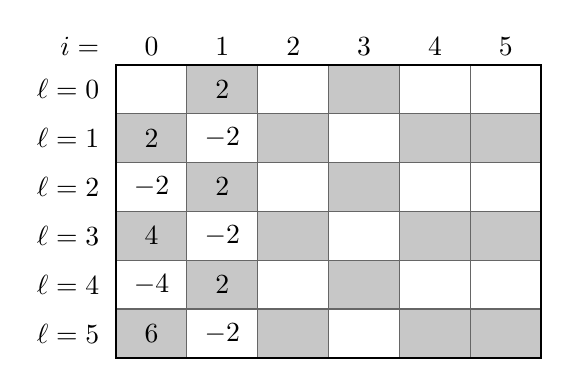
\begin{tikzpicture}[x=0.9cm,y=0.62cm]
  \fill[black!22] (1,0) rectangle (2,1);
  \node at (1.5,0.5) {$2$};
  \fill[black!22] (3,0) rectangle (4,1);
  \fill[black!22] (0,-1) rectangle (1,0);
  \node at (0.5,-0.5) {$2$};
  \node at (1.5,-0.5) {$-2$};
  \fill[black!22] (2,-1) rectangle (3,0);
  \fill[black!22] (4,-1) rectangle (5,0);
  \fill[black!22] (5,-1) rectangle (6,0);
  \node at (0.5,-1.5) {$-2$};
  \fill[black!22] (1,-2) rectangle (2,-1);
  \node at (1.5,-1.5) {$2$};
  \fill[black!22] (3,-2) rectangle (4,-1);
  \fill[black!22] (0,-3) rectangle (1,-2);
  \node at (0.5,-2.5) {$4$};
  \node at (1.5,-2.5) {$-2$};
  \fill[black!22] (2,-3) rectangle (3,-2);
  \fill[black!22] (4,-3) rectangle (5,-2);
  \fill[black!22] (5,-3) rectangle (6,-2);
  \node at (0.5,-3.5) {$-4$};
  \fill[black!22] (1,-4) rectangle (2,-3);
  \node at (1.5,-3.5) {$2$};
  \fill[black!22] (3,-4) rectangle (4,-3);
  \fill[black!22] (0,-5) rectangle (1,-4);
  \node at (0.5,-4.5) {$6$};
  \node at (1.5,-4.5) {$-2$};
  \fill[black!22] (2,-5) rectangle (3,-4);
  \fill[black!22] (4,-5) rectangle (5,-4);
  \fill[black!22] (5,-5) rectangle (6,-4);
  \foreach \x in {1,...,5} \draw[black!60] (\x,-5) -- (\x,1);
  \foreach \y in {-4,...,0} \draw[black!60] (0,\y) -- (6,\y);
  \draw[line width=0.7pt] (0,-5) rectangle (6,1);
  \node[above] at (0.5,1) {$0$};
  \node[above] at (1.5,1) {$1$};
  \node[above] at (2.5,1) {$2$};
  \node[above] at (3.5,1) {$3$};
  \node[above] at (4.5,1) {$4$};
  \node[above] at (5.5,1) {$5$};
  \node[above left] at (-0.1,1) {$i=$};
  \node[left] at (-0.1,0.5) {$\ell=0$};
  \node[left] at (-0.1,-0.5) {$\ell=1$};
  \node[left] at (-0.1,-1.5) {$\ell=2$};
  \node[left] at (-0.1,-2.5) {$\ell=3$};
  \node[left] at (-0.1,-3.5) {$\ell=4$};
  \node[left] at (-0.1,-4.5) {$\ell=5$};
\end{tikzpicture}
\caption{The $\sigma$-bump of the example at $k=6$, with $S=\{1,2,4,5\}$,
$\sigma=1$ and $Q=\{1,3\}$. Row $\ell$ holds the positions $n=6\ell+i$,
$0\le i<6$, so time runs left to right and then down. Shaded cells are the
positions in the anti-periodic set $P$, where the orbit $E$ equals $-1$;
elsewhere $E=0$. Each row is the complement of the one above, so the
pattern repeats every two rows, that is, with period $2k=12$. The numbers
are the nonzero values of the bump $d$ of \eqref{eq:trop-bump}; blank cells
have $d_n=0$. In column $1$ the bump alternates between $2$ and $-2$, while
in column $0$ it grows without bound, $d_{12m}=-2m$. Every negative entry
lies in an unshaded cell, as \eqref{eq:trop-bumpnonneg} requires.}
\label{fig:nao-bump}
\end{figure}
Consequently, by \autoref{thm:sigmabump}, no equation $x_{n+6}x_n=c_0+c_1x_{n+1}
+c_2x_{n+2}+c_4x_{n+4}+c_5x_{n+5}$ with positive $c_1,c_2,c_4,c_5$ is
globally periodic.

\subsection{The mirror}

Let $S\subseteq\{1,\dots,k-1\}$ be palindromic. If $Q$ satisfies (B1) for
$\sigma$, its reflection $Q'=k-Q$ satisfies (B1) for $k-\sigma$, and the
reflection turns a read of $1$ at the index $k-i$ for $(k-\sigma,Q')$ into a
read of $0$ at the index $i$ for $(\sigma,Q)$. This halves the work: to check
(B2) for $(\sigma,Q)$ it is enough to find a surviving tap reading $1$ at
every index, both for $(\sigma,Q)$ and for $(k-\sigma,Q')$.

\begin{lemma}[the mirror]
\label{lem:nao-mirror}
Let $S$ be palindromic, $\sigma\in S$, and let $Q,Q'\subseteq\{1,\dots,k-1\}$
satisfy $y\in Q'\iff k-y\in Q$ for $0<y<k$. If at the index $k-i$ the tap
$j'$ survives for $(k-\sigma,Q')$ and reads $v$, then at the index $i$ the tap
$k-j'$ survives for $(\sigma,Q)$ and reads $1-v$.
\end{lemma}

\begin{proof}
Let $P$ and $P'$ be the anti-periodic sets of $Q$ and $Q'$. The tap $k-j'$
lies in $S$ by palindromy. At $i$ it reads the position $p=i+k-j'$, and at
$k-i$ the tap $j'$ reads the position $p'=k-i+j'$, so $p+p'=2k$. Hence
$p\equiv-p'\pmod k$, and since $\sigma\equiv-(k-\sigma)$, the tap $k-j'$ is
deleted at $i$ exactly when $j'$ is deleted at $k-i$. For the reads, let
$r=p'\bmod k$, which is nonzero as $j'$ survives. If $p'=r$, then
$p=(k-r)+k$, so by \eqref{eq:read-antiper}
$p\in P\iff k-r\notin Q\iff r\notin Q'\iff p'\notin P'$. If $p'=r+k$, then
$p=k-r$ and $p\in P\iff k-r\in Q\iff r\in Q'\iff p'\notin P'$. Either way
the two reads are complementary.
\end{proof}

\section{Supports with at most two elements}
\label{sec:small}

This section deals with the supports with at most two elements. By
\autoref{thm:palindromy} a globally periodic equation of the form
\eqref{eq:familya} has a palindromic support, and by \autoref{lem:unfold} it
suffices to treat primitive supports. A palindromic support with at most two
elements is $\emptyset$, $\{k/2\}$ or $\{j,k-j\}$ with $1\le j<k/2$, since
$k/2$ is the only index paired with itself. Primitivity then leaves three
cases:
\begin{itemize}
\item $S=\emptyset$, which is primitive only at $k=1$. There the reciprocal
form is $x_{n+1}x_n=c_0$ with $c_0>0$, which is of known type, so there is
nothing to prove.
\item $S=\{k/2\}$, which is primitive only at $k=2$: the support $S=\{1\}$
of order two (\autoref{thm:order2}).
\item $S=\{j,k-j\}$ with $\gcd(j,k)=1$. The case $k=3j$ forces $j=1$, and
is the support $\{1,2\}$ of order three (\autoref{thm:order3}); every other
case is settled by \autoref{thm:twoterm}.
\end{itemize}

At orders two and three with $c_0>0$ neither the linearisation nor the
min-plus recursion can decide the question: at order two the characteristic
polynomial $\lambda^2-\eps_1\lambda+1$ has roots of unity whenever
$\eps_1=2\cos(2\pi q/p)$ for integers $q$ and $p\ge1$, and with $\theta=1$ the min-plus recursion is itself
periodic, with period $5$ at order two and $8$ at order three
\citep[Theorem~9]{CsornyeiLaczkovich2001}. What decides it is the second half
of \autoref{thm:P}: once round a cycle of the min-plus recursion the leading
coefficients are multiplied by a fixed factor, which must be $1$.

\subsection{Order two}

At $k=2$ with $S=\{1\}$ the equation \eqref{eq:familya} reads
\begin{equation}
x_{n+2}x_n=c_0+c_1x_{n+1},\qquad c_1>0,\quad c_0\ge0.
\label{eq:small-order2}
\end{equation}
The substitution $x_n=c_1y_n$ turns it into
\begin{equation}
y_{n+2}y_n=\alpha+y_{n+1},\qquad \alpha=\frac{c_0}{c_1^2}\ge0,
\label{eq:small-lyness}
\end{equation}
and it preserves positivity and periodicity of solutions. For $\alpha=1$
this is the Lyness equation \citep{Lyness1942}, of period $5$; for
$\alpha=0$ it has period $6$. The following theorem is known:
\citet{KocicLadasRodrigues1993} showed that the periods $5$ and $6$ occur only
for $\alpha=1$ and $\alpha=0$, and the theorem itself was proved by
\citet{BarbeauGelbordTanny1995} on the whole real plane, by
\citet{CsornyeiLaczkovich2001} with complex coefficients, and by
\citet[Theorem~3.1]{CimaGasullManosas2004}. I sketch the proof, which is
essentially that of \citet[Lemma~5]{CsornyeiLaczkovich2001} and of a remark of
\citet[Section~3]{BarbeauGelbordTanny1995}, because it is the model for order
three, where the details are given. The formalisation (\autoref{app:lean})
contains a complete proof along the lines of the sketch.

\begin{theorem}[order two]
\label{thm:order2}
If \eqref{eq:small-order2} is globally periodic, then $c_0=0$ or
$c_0=c_1^2$.
\end{theorem}

\begin{proof}[Sketch of proof]
Let $c_0>0$, so that $\alpha>0$ and $\theta=1$. The min-plus recursion
$e_{n+2}+e_n=\min(0,e_{n+1})$ started from $(e_0,e_1)=(1,0)$ runs through
the $5$-cycle $1,0,-1,-1,0$. Following the leading coefficients
\eqref{eq:trop-lead} of \autoref{thm:leading} once round this cycle, with
$c_1=1$ and constant term $\alpha$, multiplies $C_{5s+1}$ by $\alpha$: the first
two steps give $C_{5s+4}=1/C_{5s+1}$, and at $n=5s+4$ the constant slot alone
attains the minimum, so $C_{5s+6}=\alpha/C_{5s+4}=\alpha\,C_{5s+1}$. Hence
$C_{5s+1}=\alpha^s$. By \autoref{thm:P} the period $p$ is a multiple of $5$,
and $C_{p+1}=C_1$ gives $\alpha^{p/5}=1$, that is $\alpha=1$.
\end{proof}

\subsection{Order three}

At $k=3$ with $S=\{1,2\}$, \autoref{thm:palindromy} gives $c_1=c_2$ for a
globally periodic equation, so the equation is
\begin{equation}
x_{n+3}x_n=c_0+c_1(x_{n+1}+x_{n+2}),\qquad c_1>0,\quad c_0\ge0.
\label{eq:small-order3}
\end{equation}
The substitution $x_n=c_1y_n$ turns it into
\begin{equation}
y_{n+3}y_n=\alpha+y_{n+1}+y_{n+2},\qquad\alpha=\frac{c_0}{c_1^2}\ge0.
\label{eq:small-todd}
\end{equation}
For $\alpha=1$ this is the period-$8$ equation of \eqref{eq:fivefamilies}.
The following theorem is also known. With complex coefficients it follows from
Theorems~1 and~4 of \citet{CsornyeiLaczkovich2001}, and with nonnegative
coefficients it is the case $m=1$ of \citet[Theorem~4.1]{CimaGasullManosas2004};
\citet{KocicLadasRodrigues1993} had shown that the period $8$ occurs exactly
when $c_0=c_1^2$. For $c_0>0$
the proof below is that of \citet[Lemma~5(ii)]{CsornyeiLaczkovich2001}, written
in the language of \autoref{thm:leading}.

\begin{theorem}[order three]
\label{thm:order3}
If $x_{n+3}x_n=c_0+c_1x_{n+1}+c_2x_{n+2}$, with $c_1,c_2>0$ and $c_0\ge0$,
is globally periodic, then $c_1=c_2$ and $c_0=c_1^2$. In particular
$c_0>0$.
\end{theorem}

\begin{proof}
Suppose the equation is globally $p$-periodic with $p\ge1$. By
\autoref{thm:palindromy}, $c_1=c_2$, so it has the form
\eqref{eq:small-order3}. The two values of $\theta$ are handled separately.

First suppose $c_0>0$, so that \eqref{eq:small-todd} is globally
$p$-periodic with $\alpha>0$. The argument follows the sketch for order two. The min-plus
recursion is $e_{n+3}+e_n=\min(0,e_{n+1},e_{n+2})$, and the solution with initial
window $(e_0,e_1,e_2)=(1,0,-1)$ is $8$-periodic, with
\[
\begin{array}{c|cccccccc}
n\bmod8 & 0 & 1 & 2 & 3 & 4 & 5 & 6 & 7\\
\hline
e_n & 1 & 0 & -1 & -2 & -2 & -1 & 0 & 1\\
A_n & \{2\} & \{2\} & \{1,2\} & \{1\} & \{1\} & \{0,1\} & \{0\} & \{0,2\}
\end{array}.
\]
The period is exactly $8$, so \autoref{thm:P} gives $p=8r$ with $r\ge1$. If
$C_{8s}=\xi$, $C_{8s+1}=\eta$ and $C_{8s+2}=\zeta$, the eight steps
$n=8s,\dots,8s+7$ of \eqref{eq:trop-lead} give in turn
\begin{gather*}
C_{8s+3}=\frac{\zeta}{\xi},\quad
C_{8s+4}=\frac{\zeta}{\xi\eta},\quad
C_{8s+5}=\frac{\eta+1}{\xi\eta},\quad
C_{8s+6}=\frac1\eta,\quad
C_{8s+7}=\frac{\eta+1}{\zeta},\\
C_{8s+8}=\frac{\xi(\alpha\eta+1)}{\eta+1},\quad
C_{8s+9}=\alpha\eta,\quad
C_{8s+10}=\alpha\zeta .
\end{gather*}
For example, at $n=8s+2$ both taps attain, so
$C_{8s+5}C_{8s+2}=C_{8s+3}+C_{8s+4}$. Since $C_1=1$, induction gives
$C_{8s+1}=\alpha^s$, and \autoref{thm:P} gives $\alpha^r=C_{p+1}=C_1=1$. Hence
$\alpha=1$, that is $c_0=c_1^2$.

Now suppose $c_0=0$, so the equation is $x_{n+3}x_n=c_1(x_{n+1}+x_{n+2})$.
Its positive equilibrium is $x^*=2c_1$, so $\eps_1=\eps_2=\tfrac12$ in
\eqref{eq:red-ej}, and the
characteristic polynomial of \autoref{thm:spectral} is
\[
\chi(\lambda)=\lambda^3-\tfrac12\lambda^2-\tfrac12\lambda+1
=(\lambda+1)\bigl(\lambda^2-\tfrac32\lambda+1\bigr).
\]
By \autoref{thm:spectral} every root of $\chi$ is a $p$-th root of unity.
Let $\lambda$ be a root of the quadratic factor. Its discriminant is
negative, so its two roots are $\lambda$ and $\bar\lambda$, and
$\lambda\bar\lambda=1$; hence $\lambda+\lambda^{-1}=\tfrac32$. But $\lambda$
is a root of unity, hence an algebraic integer, and so is $\lambda^{-1}$;
so $\tfrac32$ would be a rational algebraic integer, that is, an integer.
This contradiction shows that $c_0=0$ is impossible.
\end{proof}

\subsection{Two-term supports}

The remaining small supports are the two-term supports $\{j,k-j\}$ at
every order.

\begin{theorem}[two-term supports]
\label{thm:twoterm}
Let $1\le j$, $2j<k$, $\gcd(j,k)=1$ and $k\ne3j$, and let $S=\{j,k-j\}$.
Then no equation \eqref{eq:familya} with support $S$ is globally periodic,
for either value of $\theta$.
\end{theorem}

Note that $\gcd(S\cup\{k\})=\gcd(j,k)$, so the hypothesis $\gcd(j,k)=1$ is
exactly primitivity of $S$; and for primitive $S$ the condition $k\ne3j$
only excludes $(k,j)=(3,1)$, the order-three support of
\autoref{thm:order3}.

Throughout this subsection, for $t\in\C$ I write
\begin{equation}
\chi_t(\lambda)=\lambda^k+1-t\,(\lambda^j+\lambda^{k-j}),
\end{equation}
which is the characteristic polynomial of \autoref{thm:spectral} for the
support $\{j,k-j\}$ with $\eps_j=\eps_{k-j}=t$. Let $\eta_1,\dots,\eta_k$
be its roots, listed with multiplicity, and let
$s_r=\sum_{i=1}^k\eta_i^r$ be their power sums.

The first step is to compute a few power sums. Because $\chi_t$ has only
four terms, Newton's identities collapse to a short recursion.

\begin{lemma}[power sums]
\label{lem:small-newton}
Let $1\le j$ and $2j<k$. Then
\begin{enumerate}
\item for $1\le r<k-j$, $s_r=j\,t^{r/j}$ if $j\mid r$, and $s_r=0$
otherwise;
\item $s_{k-j}=(k-j)\,t+t\,s_{k-2j}$;
\item $s_k=t\,(s_{k-j}+s_j)-k$.
\end{enumerate}
\end{lemma}

\begin{proof}
Write $\chi_t(\lambda)=\lambda^k+a_1\lambda^{k-1}+\dots+a_k$. Since
$1\le j<k-j<k$, the only nonzero coefficients are $a_j=a_{k-j}=-t$ and
$a_k=1$. Newton's identities
$s_r+a_1s_{r-1}+\dots+a_{r-1}s_1+r\,a_r=0$, for $1\le r\le k$, therefore
read
\[
s_r=t\,s_{r-j}\,[j<r]+t\,s_{r-(k-j)}\,[k-j<r]
+r\,t\,[r=j]+r\,t\,[r=k-j]-k\,[r=k],
\]
where $[\,\cdot\,]$ is $1$ if the condition holds and $0$ otherwise. For
$r<k-j$ only the first and third terms can be present, so $s_r=t\,s_{r-j}$
for $j<r<k-j$, $s_j=jt$ and $s_r=0$ for $r<j$; part 1 follows by
induction on $r$. Parts 2 and 3 are the cases $r=k-j$ and $r=k$, using
$k-(k-j)=j$.
\end{proof}

The power sums replace a delicate analysis of where the roots of $\chi_t$
leave the unit circle: if every $|\eta_i|=1$ then $|s_r|\le k$ for every $r$,
and for a suitable $r$ the power sum $s_r$ is an explicit function of $t$
that grows too fast.

\begin{lemma}[interval bound]
\label{lem:small-bound}
Let $1\le j$, $2j<k$, $\gcd(j,k)=1$ and $k\ne3j$, and let $t\in\C$. If
every root of $\chi_t$ has modulus $1$, then $t$ is real, $|t|\le2$ and
$t\le\sqrt2$.
\end{lemma}

\begin{proof}
First, $t$ is real. The polynomial $\chi_t$ is self-reciprocal,
$\lambda^k\chi_t(1/\lambda)=\chi_t(\lambda)$, and $\chi_t(0)=1$, so
\[
\chi_t(\lambda)=\lambda^k\chi_t(1/\lambda)=\prod_i(1-\eta_i\lambda)
=\prod_i(-\eta_i)\prod_i\bigl(\lambda-\eta_i^{-1}\bigr)
=\prod_i\bigl(\lambda-\eta_i^{-1}\bigr),
\]
since $\prod_i(-\eta_i)=\chi_t(0)=1$. So the inverses $\eta_i^{-1}$ are the roots
of $\chi_t$ again, with multiplicity. As $|\eta_i|=1$, $\eta_i^{-1}=\bar\eta_i$,
and therefore $s_j=\sum_i\eta_i^{-j}=\sum_i\bar\eta_i^{\,j}=\bar s_j$. By
\autoref{lem:small-newton}, $s_j=jt$, so $t=\bar t$ is real.

Second, $|s_r|\le\sum_i|\eta_i|^r=k$ for every $r$. Suppose $j\ge2$. Then
$0<k-2j<k-j$, and $j\nmid k-2j$, since otherwise $j\mid k$ and
$j=\gcd(j,k)=1$. By \autoref{lem:small-newton},
$s_{k-2j}=0$, $s_{k-j}=(k-j)t$, $s_j=jt$ and
\[
s_k=t\bigl((k-j)t+jt\bigr)-k=k\,(t^2-1).
\]
So $k|t^2-1|\le k$, whence $t^2\le2$, and $|t|\le\sqrt2$.

Suppose instead $j=1$. Then $k>2$ and $k\ne3$, so $k\ge4$, and
\autoref{lem:small-newton} gives $s_{k-2}=t^{k-2}$ and
$s_{k-1}=(k-1)t+t\,s_{k-2}=(k-1)t+t^{k-1}$. From the first,
$|t|^{k-2}\le k\le2^{k-2}$ (as $k\ge4$), so $|t|\le2$. From the second, if
$t>1$ then $s_{k-1}>(k-1)+1=k$, which is impossible; so $t\le1\le\sqrt2$.
\end{proof}

The last ingredient is Kronecker's theorem \citep{Kronecker1857}: if $L$ is
a number field and $\zeta\in L$ is a nonzero algebraic integer with
$|\varphi(\zeta)|\le1$ for every field embedding $\varphi:L\to\C$, then
$\zeta$ is a root of unity; for a modern account see
\citet[Theorem~1.5.9]{BombieriGubler2006}.

\begin{proof}[Proof of \autoref{thm:twoterm}]
Suppose that an equation \eqref{eq:familya} with support $S=\{j,k-j\}$ is
globally $p$-periodic. By \autoref{thm:palindromy}, $c_j=c_{k-j}$, so
$\eps_j=\eps_{k-j}=:\eps$, and \eqref{eq:red-ej} gives
$2\eps=\eps_j+\eps_{k-j}\le1$. Thus
\[
0<\eps\le\tfrac12,
\]
and by \autoref{thm:spectral} every root $\eta_i$ of $\chi_\eps$ is a
$p$-th root of unity. The idea of the proof is that $\eps=\zeta+\zeta^{-1}$
for a root of unity $\zeta$. The bound $0<\eps\le\tfrac12$ forces $\zeta$ to
have order at least $9$, and then some conjugate of $\eps$ is larger than
$\sqrt2$, which \autoref{lem:small-bound} forbids.

\emph{Step 1: $\eps$ is $\zeta+\zeta^{-1}$ for a root of unity $\zeta$.}
The coefficient of $\lambda^{k-j}$ in
$\chi_\eps=\prod_i(\lambda-\eta_i)$ is $-\eps$, and it is also $(-1)^j$
times the $j$-th elementary symmetric function of $\eta_1,\dots,\eta_k$.
Roots of unity are algebraic integers, so $\eps$ is an algebraic integer. Let $\zeta$ be a
root of $z^2-\eps z+1$; then $\zeta$ is an algebraic integer (a root of a
monic polynomial whose coefficients are algebraic integers), $\zeta\ne0$,
and $\eps=\zeta+\zeta^{-1}$. Let $L=\Q(\zeta,\eta_1,\dots,\eta_k)$,
a number field containing $\eps$. Let $\varphi:L\to\C$ be an embedding.
Applying $\varphi$ to the coefficients of
$\chi_\eps=\prod_i(\lambda-\eta_i)$ gives
$\chi_{\varphi(\eps)}=\prod_i(\lambda-\varphi(\eta_i))$, and each
$\varphi(\eta_i)$ is again a $p$-th root of unity, so of modulus $1$. By
\autoref{lem:small-bound}, $r=\varphi(\eps)$ is real with $|r|\le2$. Now
$\varphi(\zeta)$ is a root of $z^2-rz+1$, a real quadratic with
discriminant $r^2-4\le0$; its two roots are therefore complex conjugates
(or equal to $\pm1$) with product $1$, so $|\varphi(\zeta)|=1$. By
Kronecker's theorem, $\zeta$ is a root of unity.

\emph{Step 2: the order of $\zeta$.} Let $n_0$ be the order of $\zeta$.
Since $|\zeta|=1$, $\zeta^{-1}=\bar\zeta$, so
$\eps=2\cos(2\pi b/n_0)$ for some integer $b$ coprime to $n_0$, and I may
take $0\le b\le n_0/2$. Since $\cos$ is decreasing on $[0,\pi]$, with
$\cos(5\pi/12)=(\sqrt6-\sqrt2)/4>\tfrac14$ and $\cos(\pi/2)=0$, the
condition $0<\eps\le\tfrac12$ forces
\[
\frac5{24}<\frac b{n_0}<\frac14,
\]
that is, $5n_0<24b<6n_0$. If $n_0\le8$ then $24b<48$, so $b=1$ (as $b=0$ is
excluded), and $5n_0<24<6n_0$ has no integer solution. Hence $n_0\ge9$.

\emph{Step 3: a large conjugate.} The cyclotomic polynomial
$\Phi_{n_0}$ is irreducible over $\Q$, so it is the minimal polynomial of
$\zeta$, and $\e^{2\pi i/n_0}$ is another of its roots. There is therefore a
field embedding of $\Q(\zeta)$ into $\C$ sending $\zeta$ to $\e^{2\pi i/n_0}$,
and since $\zeta\in L$ it extends to an embedding $\varphi:L\to\C$. Then
\[
\varphi(\eps)=\varphi(\zeta)+\varphi(\zeta)^{-1}
=\e^{2\pi i/n_0}+\e^{-2\pi i/n_0}=2\cos(2\pi/n_0),
\]
and, as in Step 1, \autoref{lem:small-bound} gives
$2\cos(2\pi/n_0)\le\sqrt2$. But $n_0\ge9$ gives $0<2\pi/n_0<\pi/4$, so
$2\cos(2\pi/n_0)>2\cos(\pi/4)=\sqrt2$. This contradiction proves the
theorem.
\end{proof}

\section{The full support}
\label{sec:fullsupport}

The full support $S=\{1,\dots,k-1\}$ never carries a $\sigma$-bump. Indeed,
(B1) forces $Q=\{\sigma\}$, and then at $i=k-1$ every position $i+j$ with
$j\in S$ lies in $\{k,\dots,2k-2\}$, where the only position that can lie outside $P$ is
$k+\sigma$, which (B2) excludes. So the full support has to be treated on its
own. It is also the classical case: the full-support recursion, in which every
term of the window appears in the numerator, was settled, even for complex
coefficients, by \citet{CsornyeiLaczkovich2001}. They also passed to its
piecewise-linear shadow and showed, by exhibiting a non-periodic real solution
at every order other than these, that it is periodic only at order $2$ and,
with $c_0>0$, at order $3$ (their Theorems~9--11). The periods of the shadow at order $4$ with $c_0>0$ are determined by
\citet{LineroBasNievesRoldan2021}, and, with $c_0>0$, every solution with monotone initial
data has period $3k-1$ \citep{GolombCallan1992}. The carrier $Q=\{1\}$ satisfies (B1) with $\sigma=1$ but fails (B2), so the bump
is not a tangent solution along it; but every window of the full support
meets this carrier, so \autoref{lem:trop-carrier} applies, and here I give a
different unbounded tangent solution along its orbit, written down in closed
form and checked by hand.

\begin{theorem}
\label{thm:fullsupport}
Let $k\ge4$. No equation \eqref{eq:familya} with full support
$S=\{1,\dots,k-1\}$ is globally periodic, for either value of $\theta$ and for any
choice of positive coefficients.
\end{theorem}

The bound $k\ge4$ is sharp: at $k=2$ and $k=3$ the full supports $\{1\}$ and
$\{1,2\}$ carry the period-$6$, Lyness and period-$8$ equations of
\eqref{eq:fivefamilies}.

\subsection{The carrier}
\label{sec:fs-carrier}

Throughout this section $k\ge4$ and $S=\{1,\dots,k-1\}$. Let $P\subseteq\Z/2k$ be
the anti-periodic set coded by $Q=\{1\}$ (\autoref{def:bump}), that is
\[
P=\{1,\,k\}\cup\{k+2,k+3,\dots,2k-1\},
\]
and let $E$ be its orbit. Write every $n\ge0$ as $n=\ell k+i$ with $\ell\ge0$ and
$0\le i<k$, and call $\ell$ the \textit{block} and $i$ the \textit{column} of $n$.

\begin{lemma}
\label{lem:fs-carrier}
The orbit $E$ is a solution of the min-plus recursion for both values of $\theta$,
with $m_n(E)=-1$, and its attaining sets are
\[
A_{\ell k+i}(E)=\begin{cases}
\{1\}, & \ell\ \text{even},\ i=0,\\
\{k-i\}\cup\{k+2-i,\dots,k-1\}, & \ell\ \text{even},\ i\ge1,\\
\{2,\dots,k-1\}, & \ell\ \text{odd},\ i=0,\\
\{1,\dots,k-1-i\}\cup\bigl(\{k+1-i\}\cap S\bigr), & \ell\ \text{odd},\ i\ge1.
\end{cases}
\]
\end{lemma}

\begin{proof}
Let $1\le j\le k-1$. If $\ell$ is even, $n+j\equiv i+j\pmod{2k}$, with
$1\le i+j\le2k-2$. When $i+j<k$ this lies in $P$ only if $i+j=1$, that is $i=0$
and $j=1$; when $i+j\ge k$ it lies in $P$ exactly when $i+j=k$ or $i+j\ge k+2$.
If $\ell$ is odd, $n+j\equiv k+i+j\pmod{2k}$. When $i+j<k$ this lies in $P$
exactly when $i+j\ne1$, which for $j\ge1$ means $i\ge1$ or $j\ge2$; when $i+j\ge k$
the residue is $i+j-k\in\{0,\dots,k-2\}$, which lies in $P$ only if $i+j=k+1$.
This gives the four sets $\{j\in S:n+j\in P\}$ listed, and each of them is nonempty
(it contains $1$, $k-i$, $2$, and $1$ or $2$ respectively). So
\autoref{lem:trop-carrier} applies.
\end{proof}

In words, a tap $j$ at $n=\ell k+i$ reads column $i+j$ of block $\ell$ if
$i+j<k$, and column $i+j-k$ of block $\ell+1$ otherwise. So in an even block the
attaining taps read column $1$ of the same block (if $i=0$), or column $0$ and
columns $2,\dots,i-1$ of the next block (if $i\ge1$). In an odd block they read
columns $i+1,\dots,k-1$ of the same block (columns $2,\dots,k-1$ if $i=0$), and
also column $1$ of the next block when $i\ge2$. For example, at $k=5$ the
columns read by the attaining taps are as follows, a prime marking a column of
the next block:
\begin{center}
\small
\begin{tabular}{l|ccccc}
column $i$ of $n$ & $0$ & $1$ & $2$ & $3$ & $4$\\\hline
$\ell$ even & $1$ & $0'$ & $0'$ & $0',2'$ & $0',2',3'$\\
$\ell$ odd & $2,3,4$ & $2,3,4$ & $3,4,1'$ & $4,1'$ & $1'$
\end{tabular}
\end{center}
Here the middle columns are $2$ and $3$.

\subsection{The ray}

Write the block as $\ell=8m+r$ with $m\ge0$ and $0\le r<8$, so that
$n=8km+rk+i$. Define $d_n$ by \autoref{tab:fs-ray}: its value depends on $r$, on
$m$, and on the column only through the four classes $i=0$, $i=1$,
$2\le i\le k-2$ (the \textit{middle} columns) and $i=k-1$, which are distinct and
nonempty because $k\ge4$. Write $a_r$, $b_r$, $c_r$ and $z_r$ for the entries of
row $r$ in these four classes. Only the middle entries depend on $m$: they are
$f-m$ in even blocks and $f+m$ in odd blocks, for a constant $f$ given by the row.
Block $8$, which is block $0$ of the next group, has $a_8=a_0$, $b_8=b_0$,
$z_8=z_0$ and $c_8=-(m+1)$. So $d$ is a ray (\autoref{def:trop-ray}) with $q=8k$: passing from $m$ to $m+1$ changes only the
middle entries, by $-1$ in even blocks and by $+1$ in odd ones.

\begin{table}
\centering
\small
\setlength{\tabcolsep}{4pt}
\begin{tabular}{c|cccc|cccc}
$r$ & $a_r$ & $b_r$ & $c_r$ & $z_r$ &
$a_r+a_{r+1}$ & $b_r+b_{r+1}$ & $c_r+c_{r+1}$ & $z_r+z_{r+1}$\\
& $(i=0)$ & $(i=1)$ & $(2\le i\le k-2)$ & $(i=k-1)$ &&&&\\
\hline
$0$ & $-1$ & $0$ & $-m$ & $0$ & $0$ & $1$ & $1$ & $1$\\
$1$ & $1$ & $1$ & $m+1$ & $1$ & $1$ & $1$ & $0$ & $0$\\
$2$ & $0$ & $0$ & $-m-1$ & $-1$ & $0$ & $0$ & $0$ & $0$\\
$3$ & $0$ & $0$ & $m+1$ & $1$ & $1$ & $1$ & $1$ & $1$\\
$4$ & $1$ & $1$ & $-m$ & $0$ & $1$ & $0$ & $0$ & $0$\\
$5$ & $0$ & $-1$ & $m$ & $0$ & $0$ & $0$ & $0$ & $1$\\
$6$ & $0$ & $1$ & $-m$ & $1$ & $1$ & $1$ & $1$ & $1$\\
$7$ & $1$ & $0$ & $m+1$ & $0$ & $0$ & $0$ & $0$ & $0$\\
\end{tabular}
\caption{The ray of \autoref{lem:fs-ray}. Left: the value of $d_n$ at
$n=8km+rk+i$, by column class. Right: the left-hand side $d_{n+k}+d_n$ of the
tangent recursion, by column class; for $r=7$ the next block is block $0$ with $m$
replaced by $m+1$.}
\label{tab:fs-ray}
\end{table}

\begin{lemma}
\label{lem:fs-ray}
The sequence $d$ of \autoref{tab:fs-ray} is a tangent solution along $E$, for both
values of $\theta$, and $d_{8km+2k+2}=-1-m$ for every $m\ge0$.
\end{lemma}

\begin{proof}
Let $n=\ell k+i$ with $\ell=8m+r$. The left-hand side $d_{n+k}+d_n$ is the sum of
the entries of rows $r$ and $r+1$ in the class of column $i$. In the middle class
the terms in $m$ cancel, and the four sums are the right-hand half of
\autoref{tab:fs-ray}.

Now the right-hand side, the minimum of $d_{n+j}$ over $j\in A_n(E)$. Note first
that in every odd row $c_r\ge a_r$ and $c_r\ge z_r$, since $m\ge0$. By the
description after \autoref{lem:fs-carrier}, the middle columns are read only
from odd blocks, and always alongside a column whose entry is no larger: in an
even block $\ell$ at $i\ge3$ they are read from block $\ell+1$ together with its
column $0$, and in an odd block at $i\le k-3$ they are read together with column
$k-1$ of the same block. So the middle reads never lower the minimum and can be ignored,
and the right-hand side is:
\begin{itemize}
\item for $r$ even: $b_r$ if $i=0$, and $a_{r+1}$ if $i\ge1$;
\item for $r$ odd: $z_r$ if $i\in\{0,1\}$, $\min(z_r,b_{r+1})$ if
$2\le i\le k-2$, and $b_{r+1}$ if $i=k-1$.
\end{itemize}
The tangent recursion \eqref{eq:trop-tangent} therefore reduces to the identities
\[
\begin{aligned}
&r\ \text{even:}&& a_r+a_{r+1}=b_r,\quad
b_r+b_{r+1}=c_r+c_{r+1}=z_r+z_{r+1}=a_{r+1};\\
&r\ \text{odd:}&& a_r+a_{r+1}=b_r+b_{r+1}=z_r,\quad
c_r+c_{r+1}=\min(z_r,b_{r+1}),\quad z_r+z_{r+1}=b_{r+1}.
\end{aligned}
\]
These are read off \autoref{tab:fs-ray}. For the even rows $r=0,2,4,6$ the values
$(b_r;a_{r+1})$ are $(0;1)$, $(0;0)$, $(1;0)$ and $(1;1)$, and for the odd rows
$r=1,3,5,7$ the values $(z_r;\min(z_r,b_{r+1});b_{r+1})$ are $(1;0;0)$,
$(1;1;1)$, $(0;0;1)$ and $(0;0;0)$; each matches the corresponding sums. By
\autoref{lem:fs-carrier} the attaining sets, and hence this computation, are the
same for both $\theta$.

Finally, column $2$ is a middle column because $k\ge4$, so
$d_{8km+2k+2}=c_2=-1-m$.
\end{proof}

\begin{proof}[Proof of \autoref{thm:fullsupport}]
By \autoref{lem:fs-carrier} the orbit $E$ is an integer solution of the min-plus
recursion, and by \autoref{lem:fs-ray} it carries an unbounded integer tangent
solution, for both values of $\theta$. \autoref{thm:tangent} applies.
\end{proof}

\section{Odd orders}
\label{sec:oddk}

At odd order the palindromic supports have a rigid shape, and this section
uses it to dispose of every one of them except the full support.

\begin{theorem}[odd orders]
\label{thm:oddk}
Let $k$ be odd, and let $S\subseteq\{1,\dots,k-1\}$ be primitive and
palindromic with $|S|\ge3$ and $S\ne\{1,\dots,k-1\}$. Then no equation
\eqref{eq:familya} with support $S$ is globally periodic, whatever its
positive coefficients and for either value of $\theta$.
\end{theorem}

Write $k=2h+1$. Each pair $\{j,k-j\}$ contains
exactly one even number, so a palindromic support is determined by its even
elements; halving them gives a set $X\subseteq\{1,\dots,h\}$ with
\begin{equation}
S=\{\,2x,\ k-2x\ :\ x\in X\,\}.
\label{eq:odd-coords}
\end{equation}
Two quite different mechanisms are needed, according to whether or not $X$
is a \emph{dilated interval}, that is $X=\mu\cdot\{1,\dots,M\}$ for some
integers $\mu,M\ge1$.
If $X$ is not a dilated interval (\autoref{sec:odd-nondil}), an unbounded
tangent solution along a fixed periodic orbit, which alternates between low
values at odd positions and high values at even ones, can be written down in
closed form; whether it exists turns on rigidity statements about
translates and reflections of $X$ modulo $k$, which fail only for dilated
intervals. If $X$ is a dilated interval (\autoref{sec:odd-dil}), the support
carries a $\sigma$-bump. The first mechanism cannot simply be replaced by
the second. At $k=7$ there are
exactly two primitive palindromic supports with a non-dilated $X$,
$\{1,2,5,6\}$ and $\{1,3,4,6\}$, and neither carries a
$\sigma$-bump, as one can check by running through the four choices of
$\sigma$ and the $2^7$ anti-periodic sets; this explains the choice of
method, but it is not used in the proof and is not formalised. The tangent
solutions along the alternating orbit give a short uniform argument instead, and the
$\sigma$-bump is used only where rigidity fails, for the dilated intervals.

The alternating orbit has a precedent in the work of
\citet{CimaGasullManosas2004}. At odd order a palindromic equation has a
one-parameter family of $2$-periodic solutions, equal to $t$ at even and
$(st+c_0)/(t-s)$ at odd positions, where $t>s=\sum_{j\in S,\,j\text{ even}}c_j$;
along it the eigenvalues of the derivative of the second iterate must be
constant roots of unity \citep[Proposition~2.6]{CimaGasullManosas2004}, which
gives polynomial conditions on the coefficients that they solve at
$k=5,7,9,11$. Taking $t-s$ a fixed multiple of $\delta^3$ and letting
$\delta\to0^+$ gives the $2$-periodic min-plus solution equal to $0$ at even
and $-3$ at odd positions, and the alternating orbit below changes it at two
positions in each period $2k$. The mechanism here is different, however: the
tangent recursion along the alternating orbit depends only on $S$, so it
disposes of every choice of coefficients at once.

Throughout, $k=2h+1$ is odd, and residues modulo $k$ are identified with
their representatives in $\{0,\dots,k-1\}$; for a residue $n$ and a set $X$
of residues, $n+X$ and $n-X$ denote the translate and the reflection of $X$
taken modulo $k$. The set $X$ always lies in the lower half
$\{1,\dots,h\}$, and two elementary facts about such sets are used
repeatedly: for $x,y\in X$,
\begin{equation}
x+y\not\equiv0\pmod k,
\qquad\text{and}\qquad
-x\equiv k-x\in\{h+1,\dots,2h\}\ \text{lies outside } X\cup\{0\},
\label{eq:odd-half}
\end{equation}
because $2\le x+y\le 2h<k$. I write $\mathbf 1[\,\cdot\,]$ for the indicator
of a statement, equal to $1$ if it is true and $0$ otherwise, and
$\mathbf 1_U(y)=\mathbf 1[\,y\in U\,]$ for the indicator function of a set
$U$.

\begin{lemma}[coordinates]
\label{lem:odd-coords}
Let $S\subseteq\{1,\dots,k-1\}$ be palindromic, and put
$X=\{s/2:\ s\in S\text{ even}\}$. Then $X\subseteq\{1,\dots,h\}$,
\eqref{eq:odd-coords} holds, and $|S|=2|X|$. In particular $|S|\ge3$ forces
$|X|\ge2$, and then $S$ contains at least two odd elements.
\end{lemma}

\begin{proof}
By palindromy $S$ is the union of pairs $\{j,k-j\}$, each consisting of one
even element $2x\le 2h$ and one odd element $k-2x$, and these $2|X|$ numbers
are distinct.
\end{proof}

\subsection{The alternating orbit and the reduced recursion}
\label{sec:odd-carrier}

The periodic orbit used below alternates, low on odd positions and high on
even ones, except for a single raised value at one odd position of each
period $2k$, compensated a half-period later. For $n\ge0$ put
\begin{equation}
E_n=\begin{cases}
-2 & n \text{ odd},\ n\equiv1 \pmod{2k},\\
-3 & n \text{ odd},\ n\not\equiv1 \pmod{2k},\\
-1 & n \text{ even},\ n\equiv k+1 \pmod{2k},\\
\phantom{-}0 & n \text{ even},\ n\not\equiv k+1 \pmod{2k}.
\end{cases}
\end{equation}
I call $E$ the \emph{alternating orbit}.

\begin{lemma}[the alternating orbit]
\label{lem:odd-carrier}
Let $S$ be palindromic with at least two odd elements. Then $E$ is a
$2k$-periodic integer solution of the min-plus recursion with support $S$,
for either value of $\theta$: $E_{n+k}+E_n=-3$ for every $n$, the minimum
over the slots at time $n$ is $-3$, and it is attained exactly at the taps
\begin{equation}
A_n=\{\,j\in S\ :\ n+j \text{ odd},\ n+j\not\equiv1\pmod{2k}\,\};
\end{equation}
the constant slot, when $\theta=1$, never attains.
\end{lemma}

\begin{proof}
As $k$ is odd, $n$ and $n+k$ have opposite parities, and $n\equiv1$ exactly
when $n+k\equiv k+1 \pmod{2k}$; so the two exceptional values $-2$ and $-1$
are always paired, and $E_{n+k}+E_n=-3$ in every case. Every value of $E$ is
at least $-3$, with equality exactly at the odd positions other than those
$\equiv1\pmod{2k}$, and the constant slot is worth $0>-3$. It remains to see
that $A_n$ is nonempty. If $n$ is even, $A_n$ consists of the odd taps $j$
with $n+j\not\equiv1$; there are at least two odd taps and at most one of
them has $n+j\equiv1\pmod{2k}$. If $n$ is odd, the same argument applies to
the even taps, of which there are as many as odd ones.
\end{proof}

The tangent recursion along $E$ is
\begin{equation}
d_{n+k}+d_n=\min_{j\in A_n} d_{n+j}\qquad(n\ge0),
\label{eq:odd-tangent}
\end{equation}
and every tap in $A_n$ reads $d$ at an odd position. So the values of $d$ at
odd positions should determine everything, and they do. Write
$v_t=d_{2t+1}$, and use the coordinates \eqref{eq:odd-coords}. At the odd
time $n=2t+1$ the attaining taps are the even ones, $j=2x$, which read
$d_{2(t+x)+1}=v_{t+x}$ and are absent when $2(t+x)+1\equiv1\pmod{2k}$, that
is when $t+x\equiv0\pmod k$. At the even time $n=2t+1+k$ they are the odd
ones, $j=k-2x$, which read $v_{t+k-x}$ and are absent when $t-x\equiv0\pmod
k$. This motivates the two \emph{read sets}, of the time $2t+1$ and of the
time $2t+1+k$ half a period later,
\begin{equation}
R_+(t)=\{\,t+x\ :\ x\in X,\ t+x\not\equiv0\,\},
\qquad
R_-(t)=\{\,t+k-x\ :\ x\in X,\ t-x\not\equiv0\,\},
\label{eq:odd-reads}
\end{equation}
with congruences modulo $k$; these are sets of positive integers. Modulo $k$,
$R_+(t)$ lies in the translate $t+X$ and $R_-(t)$ in the reflection $t-X$,
which explains the signs. Each is nonempty when $|X|\ge2$,
since at most one $x\in X$ can satisfy $t\pm x\equiv0$. Note that no read
ever lands on a multiple of $k$: the tap that would have done so is exactly
the one that is absent. The \emph{reduced recursion} is
\begin{equation}
v_{t+k}-v_t=\min_{y\in R_-(t)}v_y-\min_{y\in R_+(t)}v_y\qquad(t\ge0).
\label{eq:odd-vrec}
\end{equation}

\begin{proposition}[reduction to the odd positions]
\label{prop:odd-second}
Let $S$ be palindromic with $|S|\ge3$, with $X$ as in \autoref{lem:odd-coords}.
If the reduced recursion \eqref{eq:odd-vrec} has an unbounded integer
solution $(v_t)_{t\ge0}$, then no equation \eqref{eq:familya} with support
$S$ is globally periodic, for any positive coefficients and either $\theta$.
\end{proposition}

\begin{proof}
Define $d_n$ for $n\ge0$ by $d_{2t+1}=v_t$ at odd positions, and at even
positions by
\[
d_n=\min_{j\in A_n}d_{n+j}-d_{n+k}\qquad(n\text{ even});
\]
the right-hand side involves only odd positions ($n+j$ for odd $j$, and
$n+k$), so this is a definition. Then \eqref{eq:odd-tangent} holds at every
even $n$ by construction. At an odd time $n=2t+1$ the position $n+k$ is even,
so by the definition and the description of the attaining taps above,
\[
d_{n+k}=\min_{j\in A_{n+k}}d_{n+k+j}-d_{n+2k}=\min_{y\in R_-(t)}v_y-v_{t+k},
\]
and hence
$d_{n+k}+d_n=\min_{R_-(t)}v-v_{t+k}+v_t=\min_{R_+(t)}v
=\min_{j\in A_n}d_{n+j}$ by \eqref{eq:odd-vrec}. So $d$ is an integer
solution of the tangent recursion along the alternating orbit $E$ of
\autoref{lem:odd-carrier}, which applies because $|X|\ge2$; and $d$ is
unbounded because $v$ is. The conclusion is \autoref{thm:tangent}.
\end{proof}

\subsection{Rays}
\label{sec:odd-rays}

The unbounded solutions of the reduced recursion used below are
\emph{rays of the reduced recursion}: they satisfy
$v_{t+k}=v_t+\Delta(t\bmod k)$ for a fixed function $\Delta$ on $\Z/k$, not
identically zero. Only residues modulo $k$ matter for the read sets
\eqref{eq:odd-reads}: the residues of $R_+(t)$ and $R_-(t)$ are
\begin{equation}
\bar R_+(r)=(r+X)\setminus\{0\},
\qquad
\bar R_-(r)=(r-X)\setminus\{0\},
\qquad r=t\bmod k,
\end{equation}
the punctured translate and the punctured reflection of $X$. For a set
$U\subseteq\Z/k$, say that $r$ is \emph{reflection-blocked} if
$\bar R_-(r)\subseteq U$, and \emph{translate-blocked} if
$\bar R_+(r)\subseteq U$.

\begin{lemma}[indicator rays]
\label{lem:odd-ray}
Let $|X|\ge2$ and $U\subseteq\Z/k\setminus\{0\}$, and define
$\Delta:\Z/k\to\Z$ by
\begin{equation}
\Delta(r)=\mathbf 1[\,r\text{ reflection-blocked}\,]-\mathbf 1[\,r\text{ translate-blocked}\,].
\label{eq:odd-raycond}
\end{equation}
Suppose that $0$ is translate-blocked and not reflection-blocked, that no
$r\ne0$ is translate-blocked, and that every reflection-blocked $r$ lies in
$U$. Suppose also the \emph{vanishing condition}: every blocked read set, that
is $\bar R_-(r)$ for $r$ reflection-blocked and $\bar R_+(r)$ for $r$
translate-blocked, contains a residue at which $\Delta$ vanishes. Then
\[
v_t=\mathbf 1_U(t\bmod k)-\mathbf 1[\,t\equiv0\,]+\lfloor t/k\rfloor\,\Delta(t\bmod
k)\qquad(t\ge0)
\]
solves the reduced recursion \eqref{eq:odd-vrec}, and $v_{mk}=-1-m$, so $v$
is unbounded.
\end{lemma}

\begin{proof}
The hypotheses say that $\Delta(0)=-1$, that $\Delta\ge0$ elsewhere, and
that $\Delta=0$ outside $U\cup\{0\}$. Clearly $v_{t+k}-v_t=\Delta(t\bmod k)$,
and $v_{mk}=-1-m$ because $0\notin U$.
Now look at the value of $v$ at a read $y$, whose residue $\rho=y\bmod k$ is
never $0$, by \eqref{eq:odd-reads}. If $\rho\notin U$ then $\Delta(\rho)=0$ and $v_y=0$. If $\rho\in
U$ then $v_y=1+\lfloor y/k\rfloor\Delta(\rho)\ge1$, with equality when
$\Delta(\rho)=0$. Hence the minimum of $v$ over a read set is $0$ if some
read lies outside $U$, and is exactly $1$ if all reads lie in $U$, that is,
if the read set is blocked; in that case the vanishing condition supplies a
read with $\Delta(\rho)=0$. So the right-hand side of \eqref{eq:odd-vrec} is
$\mathbf 1[\,r\text{ reflection-blocked}\,]-\mathbf 1[\,r\text{ translate-blocked}\,]$
with $r=t\bmod k$, which is $\Delta(r)$.
\end{proof}

\begin{remark}[the tangent solution is a ray]
\label{rem:odd-ray2k}
This remark is not used in the proof of \autoref{thm:oddk}. For a solution
$v$ as in \autoref{lem:odd-ray}, the tangent solution $d$ built from $v$ in
the proof of \autoref{prop:odd-second} is a ray in the sense of
\autoref{def:trop-ray}, with $q=2k$. At odd positions,
$d_{2t+1+2k}=v_{t+k}=v_t+\Delta(t\bmod k)$. At an even position $n$, write
$n+k=2\tau+1$; there $d_n$ is the minimum of $v$ over a read set, less
$d_{n+k}=v_\tau$. By the proof of \autoref{lem:odd-ray}, that minimum is $0$
or $1$ and depends only on the residues read, which do not change when $n$
increases by $2k$; so $d_{n+2k}=d_n-\Delta(\tau\bmod k)$. Thus
$d_{n+2k}=d_n+u_n$ with $u$ $2k$-periodic, and $u$ is not identically zero
since $\Delta(0)=-1$.
\end{remark}

The whole difficulty is to choose $U$ so that the blocking hypotheses hold,
and for that one needs to know when a punctured translate or reflection of $X$ can lie inside
$X$ or a slight enlargement of it.

\subsection{Rigidity of translates and reflections}
\label{sec:odd-rigid}

Say that $X$ is \emph{symmetric about} $j\in\Z/k$ if $j-X\subseteq X$
(equivalently $j-X=X$), and that $W=X\cup\{0\}$ is \emph{symmetric about}
$z$ if $z\in X$ and $z-x\in X$ for every $x\in X\setminus\{z\}$ (equivalently
$z-W=W$). The first three statements below conclude that $X$ is a dilated
interval.

\begin{lemma}[translate rigidity]
\label{lem:odd-trigid}
Let $\emptyset\ne X\subseteq\{1,\dots,h\}$ and $\zeta\not\equiv0\pmod k$.
If $\zeta+X\subseteq X\cup\{0\}$ modulo $k$, then $X$ is a dilated interval.
\end{lemma}

\begin{proof}
Take $0<\zeta<k$. If $\zeta\le h$, then for $x_{\max}=\max X$ the integer
$x_{\max}+\zeta$ lies in $(x_{\max},2h]$, so modulo $k$ it is neither $0$
nor an element of $X$; hence $\zeta>h$. Put $\mu=k-\zeta\in\{1,\dots,h\}$, so
that translation by $\zeta$ is $x\mapsto x-\mu$ modulo $k$. For $x\in X$ with
$x<\mu$, the residue $x-\mu+k$ lies in $\{h+1,\dots,2h\}$ and is neither $0$
nor in $X$; so every $x\in X$ has $x\ge\mu$ and $x-\mu\in X\cup\{0\}$. By
induction every element of $X$ is a multiple of $\mu$, and stepping down
from $\max X=M\mu$ by $\mu$ stays inside $X$ until it reaches $0$; so
$X=\mu\cdot\{1,\dots,M\}$.
\end{proof}

\begin{lemma}[translates of a symmetric set]
\label{lem:odd-symfail}
Let $\emptyset\ne X\subseteq\{1,\dots,h\}$ be symmetric about $j$, and let
$\zeta\not\equiv0$. If $\zeta+X\subseteq X\cup\{0,j\}$, then $X$ is a dilated
interval.
\end{lemma}

\begin{proof}
The translate can leave $X$ only at $0$ and at $j$. It cannot leave at both:
if $x_1+\zeta\equiv0$ and $x_2+\zeta\equiv j$ with $x_1,x_2\in X$, then
$y=j-x_2\in X$ and $y\equiv\zeta\equiv-x_1$, against \eqref{eq:odd-half}. If
it never leaves at $j$, \autoref{lem:odd-trigid} applies directly. If it
leaves only at $j$, reflect: for $y\in X$ put $x=j-y\in X$. Either
$x+\zeta\in X$, and then $y-\zeta=j-(x+\zeta)\in X$; or $x+\zeta\equiv j$, and
then $y-\zeta\equiv0$. So $-\zeta+X\subseteq X\cup\{0\}$, and
\autoref{lem:odd-trigid} applies to $-\zeta$.
\end{proof}

\begin{lemma}[uniqueness of the centre of $W$]
\label{lem:odd-wunique}
Let $\emptyset\ne X\subseteq\{1,\dots,h\}$. If $W=X\cup\{0\}$ is symmetric
about two distinct residues $z$ and $z'$, then $X$ is a dilated interval.
\end{lemma}

\begin{proof}
Put $\zeta=z'-z\not\equiv0$; I check $\zeta+X\subseteq X\cup\{0\}$ and apply
\autoref{lem:odd-trigid}. For $x=z$, $x+\zeta=z'\in X$. For $x\ne z$, $y=z-x$
lies in $X$, and $x+\zeta=z'-y$; this is $0$ if $y=z'$, and lies in $X$
otherwise, by the symmetry of $W$ about $z'$.
\end{proof}

Finally, reflection blocking against $X$ itself is always a symmetry.

\begin{lemma}[reflection blocking]
\label{lem:odd-frigid}
If $(r-X)\setminus\{0\}\subseteq X$, then $X$ is symmetric about $r$ or $W$
is symmetric about $r$.
\end{lemma}

\begin{proof}
If $r\notin X$ then no $r-x$ vanishes, and $r-X\subseteq X$. If $r\in X$
then $r-x\not\equiv0$ for every $x\in X\setminus\{r\}$, so $r-x\in X$ for all
such $x$, which is the symmetry of $W$ about $r$.
\end{proof}

\subsection{The non-dilated sets}
\label{sec:odd-nondil}

\begin{theorem}[non-dilated sets]
\label{thm:odd-nondil}
Let $S$ be palindromic with $|S|\ge3$, and suppose that the set $X$ of
\autoref{lem:odd-coords} is not a dilated interval. Then no equation
\eqref{eq:familya} with support $S$ is globally periodic, for any positive
coefficients and either $\theta$.
\end{theorem}

\begin{proof}
By \autoref{prop:odd-second} and \autoref{lem:odd-ray} it suffices to
exhibit $U$ satisfying the hypotheses of \autoref{lem:odd-ray}. Here
$|X|\ge2$ by \autoref{lem:odd-coords}. If $X$ is symmetric about some $j$, then $j\ne0$, since $-X$ is
disjoint from $X$ by \eqref{eq:odd-half}, and $j\notin X$, since otherwise
$0=j-j\in X$; take $U=X\cup\{j\}$. Otherwise take $U=X$. In both cases $0$ is
translate-blocked, since $\bar R_+(0)=X$, and no $r\ne0$ is translate-blocked:
blocking would mean $r+X\subseteq U\cup\{0\}$, and \autoref{lem:odd-trigid}
or \autoref{lem:odd-symfail} would make $X$ a dilated interval. It remains to
find the reflection-blocked residues and to check the vanishing condition.

\emph{$U=X\cup\{j\}$.} Reflection blocking happens exactly at $r=j$, which
lies in $U$. Indeed $\bar R_-(j)=j-X=X\subseteq U$. At $r=0$, $\bar R_-(0)=-X$ has at least two elements,
none in $X$, so they cannot all equal $j$. At $r\notin\{0,j\}$, put
$\zeta=r-j\not\equiv0$; for $y\in X$, the residue $x=j-y$ lies in $X$ and
$y+\zeta=r-x$, so reflection blocking at $r$ would give
$\zeta+X\subseteq X\cup\{0,j\}$, and \autoref{lem:odd-symfail} would make $X$
a dilated interval. So $\Delta=\mathbf 1_{\{j\}}-\mathbf 1_{\{0\}}$, and the
two blocked read sets are $\bar R_-(j)=X$ and $\bar R_+(0)=X$, on which
$\Delta$ vanishes.

\emph{$U=X$.} The residue $0$ is not reflection-blocked, since $-X$ is
disjoint from $X$. If $r$ is reflection-blocked, \autoref{lem:odd-frigid}
makes $X$ or $W$ symmetric about $r$; the first is excluded, so $W$ is
symmetric about $r$, which puts $r$ in $X=U$. By \autoref{lem:odd-wunique}
there is at most one such $r$. So $\Delta$ vanishes on all of $X$ except at
most one point, and $\bar R_+(0)=X$, having at least two elements, contains a
zero of $\Delta$. If $z$ is reflection-blocked, then for $x\in X$ with $x\ne z$
the read $z-x\in\bar R_-(z)$ is neither $0$ nor $z$, so $\Delta(z-x)=0$; such
an $x$ exists as $|X|\ge2$, so $\bar R_-(z)$ also contains a zero of
$\Delta$. This is the vanishing condition.
\end{proof}

\subsection{Dilated intervals}
\label{sec:odd-dil}

When $X=\mu\cdot\{1,\dots,M\}$ the support is
\begin{equation}
S=\{\,2\mu i,\ k-2\mu i\ :\ 1\le i\le M\,\},\qquad 2\mu M\le 2h<k,
\label{eq:odd-prog}
\end{equation}
and the rigidity lemmas of \autoref{sec:odd-rigid} no longer rule out
blocking. These supports carry a $\sigma$-bump with $\sigma$ even. Since $k$
is odd, every residue modulo $2k$ is uniquely of the form $2u$ or $2u+k$ with
$u\in\Z/k$, so an anti-periodic set is the same thing as a function on
$\Z/k$, and (B1) and (B2) become conditions on translates and reflections of
$X$.

For $s\in\Z/k$, the translate $s+X$ and the reflection $s-X$ are called the
two \emph{runs} at $s$.

\begin{lemma}[carriers on $\Z/k$]
\label{lem:odd-fold}
Let $S$ be palindromic, with $X$ as in \autoref{lem:odd-coords}, and let
$x_0\in X$ and $\sigma=2x_0$. For $\gamma:\Z/k\to\{0,1\}$ let $P_\gamma$ be
the set of residues modulo $2k$ of the form $2u$ with $\gamma(u)=1$ or $2u+k$
with $\gamma(u)=0$. Then $P_\gamma$ is anti-periodic, every anti-periodic set
is $P_\gamma$ for exactly one $\gamma$, and $(\sigma,P_\gamma)$ is a
$\sigma$-bump for $S$ if and only if
\begin{enumerate}
\item[(F1)] $\gamma(0)=0$, $\gamma(x_0)=1$, $\gamma(x)=0$ for
$x\in X\setminus\{x_0\}$, and $\gamma(-x)=1$ for $x\in X$;
\item[(F2)] for every $s\in\Z/k\setminus\{0\}$, the values $\gamma(u)$ for
$u$ in the run $s+X$ and $1-\gamma(u)$ for $u$ in the run $s-X$, with
$u\notin\{0,x_0\}$,
include both $0$ and $1$.
\end{enumerate}
\end{lemma}

\begin{proof}
As $k$ is odd, $u\mapsto 2u$ is a bijection from $\Z/k$ onto the even
residues modulo $2k$, and $u\mapsto2u+k$ onto the odd ones. Write
$g(n)=\mathbf 1[\,n\in P\,]$ for a set $P$ of residues modulo $2k$. For
$P=P_\gamma$, $g(2u)=\gamma(u)$ and $g(2u+k)=1-\gamma(u)$, so $P_\gamma$ is
anti-periodic. Conversely, if $P$ is anti-periodic, then with
$\gamma(u)=g(2u)$ one gets $g(2u+k)=1-\gamma(u)$, so $P=P_\gamma$, and
$\gamma$ is determined by $P$.

\emph{(B1).} The position $0=2\cdot0$ lies in $P_\gamma$ iff $\gamma(0)=1$,
the even tap $2x$ lies in $P_\gamma$ iff $\gamma(x)=1$, and the
odd tap $k-2x=2(-x)+k$ lies in $P_\gamma$ iff $\gamma(-x)=0$. So
$P_\gamma\cap(\{0\}\cup S)=\{\sigma\}$ says exactly (F1).

\emph{(B2).} Let $0<i<k$, and let $s\in\Z/k$ be the residue with
$2s\equiv i\pmod k$; then $s\ne0$, and $i\mapsto s$ is a bijection from
$\{1,\dots,k-1\}$ onto $\Z/k\setminus\{0\}$. By the Chinese remainder
theorem $i\equiv2s\pmod{2k}$ if $i$ is even and $i\equiv2s+k$ if $i$ is
odd. So for $x\in X$ the tap $2x$ reads the position
$i+2x\equiv2(s+x)$ or $2(s+x)+k$, and the tap $k-2x$ reads
$i+k-2x\equiv2(s-x)+k$ or $2(s-x)$. When $i$ is even the reads are therefore
$\gamma(s+x)$ and $1-\gamma(s-x)$, and when $i$ is odd they are the
complements of these. The tap $2x$ is deleted when $i+2x\equiv0$ or
$i+2x\equiv\sigma=2x_0\pmod k$, that is when $s+x\equiv0$ or $x_0$, since $2$ is a unit
modulo $k$; likewise the tap $k-2x$ is deleted when $s-x\equiv0$ or $x_0$.
Complementing every read does not change whether both values occur, so
(B2) at $i$ is (F2) at $s$.
\end{proof}

A unit modulo $k$ carries the conditions (F1) and (F2) from one set to
another. Indeed, let $\mu$ be a unit modulo $k$, let $X'=\mu X$ and
$x_0'=\mu x_0$, and put $\gamma'(u)=\gamma(\mu^{-1}u)$. The map
$u\mapsto\mu^{-1}u$ fixes $0$, carries $x_0'$ to $x_0$ and $X'$ to $X$, and
carries the runs $s\pm X'$ to the runs $\mu^{-1}s\pm X$, with
$\mu^{-1}s\ne0$ when $s\ne0$. So if $\gamma$ satisfies (F1) and (F2) for
$(X,x_0)$, then $\gamma'$ satisfies them for $(X',x_0')$. This reduces the
dilated intervals to $X=\{1,\dots,M\}$ and $x_0=1$, where the following
explicit function works.

\begin{theorem}[the interval carrier]
\label{thm:odd-rowcarrier}
Let $k=2h+1$ be odd and $M\ge2$ with $2M+3\le k$, and represent the residues
modulo $k$ by $u\in[-h,h]$. Define $\gamma:\Z/k\to\{0,1\}$ by
\[
\gamma(0)=0,\quad \gamma(1)=1,\quad \gamma(u)=0\ (2\le u\le M),\quad
\gamma(-u)=1\ (1\le u\le M),
\]
\[
\gamma(u)=\mathbf 1[\,u\equiv M+1\pmod 2\,],\qquad \gamma(-u)=1-\gamma(u)
\qquad(M<u\le h).
\]
Then $\gamma$ satisfies (F1) and (F2) for $X=\{1,\dots,M\}$ and $x_0=1$.
\end{theorem}

\begin{proof}
Here $h\ge M+1\ge3$, so the five sets $\{0\}$, $[1,M]$, $[-M,-1]$,
$I_+=[M+1,h]$ and $I_-=[-h,-M-1]$ partition $[-h,h]$, and $\gamma$ is well
defined. Condition (F1) holds by construction. Call the residues $0$ and $1$
\emph{excluded}; they are the residues removed in (F2). The function $\gamma$
has three properties.
\begin{itemize}
\item[(i)] $\gamma(-u)=1-\gamma(u)$ for $2\le u\le h$: for $u\le M$ both
sides are $1$, and for $u>M$ this is the definition.
\item[(ii)] $\gamma$ changes value between $M$ and $M+1$, between $-M-1$ and
$-M$, and between $h$ and $h+1\equiv-h$. Indeed $\gamma(M)=0$ and
$\gamma(M+1)=1$, $\gamma(-M)=1$ and $\gamma(-M-1)=0$ by (i), and
$\gamma(-h)=1-\gamma(h)$ by (i).
\item[(iii)] $\gamma$ takes both values on any two consecutive residues of
$I_+$, since exactly one of them is $\equiv M+1\pmod 2$, and likewise of
$I_-$, by (i).
\end{itemize}
Also $\gamma(-1)=1\ne0=\gamma(2)$.

Going round $\Z/k$, the residues fall into the consecutive arcs $[2,M]$, $I_+$, $I_-$, $[-M,-1]$, followed by the excluded
pair $\{0,1\}$ and then $[2,M]$ again. By (ii) and the last remark, $\gamma$
changes value between the last residue of each of the four arcs and the
first residue of the next (across the excluded pair, between $-1$ and $2$).
So if $\gamma$ is constant on the non-excluded elements of a run $R$ of $M$
consecutive residues, then $R$ meets only one of the four arcs, since an
arc of fewer than $k$ residues that meets two of them contains a boundary
pair. It cannot lie in $I_\pm$, by (iii), as $M\ge2$; so $R\subseteq[-M,1]$
or $R\subseteq[0,M]$.

Suppose now that (F2) fails at $s\ne0$. Then $\gamma$ is constant on the
non-excluded elements of both runs. The run $s+\{1,\dots,M\}$ lies in
$[-M,1]$ or in $[0,M]$, which forces $s\in[-M-1,1-M]$ or $s\in\{-1,0\}$; the
run $s-\{1,\dots,M\}$ likewise forces $s\in\{0,1,2\}$ or $s\in\{M,M+1\}$.
All these residues lie in $[-M-1,M+1]$, whose $2M+3\le k$ elements are
distinct modulo $k$. The first list lies in $[-M-1,0]$ and the second in
$\{0\}\cup[1,M+1]$, so the only residue in both is $0$. This contradicts
$s\ne0$.
\end{proof}

\subsection{Proof of \autoref{thm:oddk}}
\label{sec:odd-proof}

\begin{proof}[Proof of \autoref{thm:oddk}]
Let $k=2h+1$ and $S$ be as in the theorem, and let $X$ be as in
\autoref{lem:odd-coords}, so that $|X|\ge2$. If $X$ is not a dilated interval,
\autoref{thm:odd-nondil} applies. Otherwise $X=\mu\cdot\{1,\dots,M\}$, and
$S$ is \eqref{eq:odd-prog}, with $M=|X|\ge2$ and $2\mu M\le2h$. Every element
of $S$ is $2\mu i$ or $k-2\mu i$, so $\gcd(\mu,k)$ divides every element of
$S\cup\{k\}$, and primitivity gives $\gcd(\mu,k)=1$. If $\mu=1$ and $M=h$,
then $S$ is the full support, which is excluded. If $\mu=1$ and $M\le h-1$,
then $2M+3\le k$. If $\mu\ge2$, then $4M\le2\mu M<k$, and $2M+3\le4M<k$ since
$M\ge2$. In either of the last two cases \autoref{thm:odd-rowcarrier} gives a
function satisfying (F1) and (F2) for $\{1,\dots,M\}$ and $1$; multiplying
its argument by $\mu^{-1}$ modulo $k$, as above, gives one for $X$ and
$x_0=\mu$, and \autoref{lem:odd-fold} turns it into a $2\mu$-bump for $S$.
\autoref{thm:sigmabump} now shows that no equation with support $S$ is
globally periodic, for any positive coefficients and either $\theta$.
\end{proof}

\section{Even orders: supports with an even element}
\label{sec:notallodd}

Throughout this section the order $k$ is even. With \autoref{thm:sigmabump},
the following theorem disposes of every support at even order, other than the
full support, that is not all-odd. Reads are described in the vocabulary of
\autoref{sec:nao-reading}, in particular \eqref{eq:read-reads} and
\eqref{eq:read-pins}, and \autoref{lem:nao-mirror} turns reads of $1$ into
reads of $0$.

\begin{theorem}
\label{thm:notallodd}
Let $k$ be even and let $S\subseteq\{1,\dots,k-1\}$ be primitive and
palindromic, not the full support, and containing an even element. Then
$S$ carries a $\sigma$-bump $(\sigma,P)$.
\end{theorem}

The natural carriers at even order are the \emph{parity carriers}: $\sigma$
together with every free residue that has the parity of $\sigma$. Because $k$ is even, the reflection $y\mapsto k-y$ preserves
parity, and the argument splits along the two parity classes. Under (B1) the
reads of the pins are fixed by \eqref{eq:read-pins}, and a parity carrier puts every free position of one class
into $Q$, so an unwrapped tap that lands on a free position of that class
reads $1$. A clause can therefore fail, for $\sigma$ or (by a reflection) for
$k-\sigma$, only at an index $i$ where every unwrapped tap of the right class
lands back in $S$, so that $S$ is almost closed under adding $i$. If
$a=\min S$ is even, a failure of the odd class forces a gap in the even part
of $S$, and taps reading into that gap make the even class work for every
even $\sigma$ (\autoref{thm:nao-evenmin}). If $a$ is odd and both classes
fail for every $\sigma$, the failures force a rigid progression structure
(\autoref{thm:nao-struct}), which carries one of two explicit carriers at
$\sigma=a$ (Lemmas~\ref{lem:nao-bfone} and~\ref{lem:nao-bfshadow}). On a
first reading one can take Lemmas~\ref{lem:nao-noband},
\ref{lem:nao-endend} and~\ref{lem:nao-endband} on trust.

\subsection{Parity carriers}
\label{sec:nao-parity}

Write $S_0$ and $S_1$ for the even and odd elements of $S$, and refer to the
residue of an integer modulo $2$ as its \emph{class}. Since $k$ is even,
$s\equiv k-s\pmod2$ for every integer $s$, so $S_0$ and $S_1$ are each
palindromic, and a nonempty class $S_c$ has largest element $k-\min S_c$.
If $S$ is primitive then $S_1\ne\emptyset$, since otherwise $2$ would divide
every element of $S\cup\{k\}$.

\begin{definition}
For $\sigma\in S$, the \emph{parity carrier} of $\sigma$ is
\[
Q_\sigma=\{\sigma\}\cup\{\,y\in\{1,\dots,k-1\}:\ y\notin S,\ y\equiv \sigma
\pmod2\,\}.
\]
An index $i$ is \emph{silent} for $Q_\sigma$ if no surviving tap reads $1$
at $i$. For an index $i$ and a class $c$, write $C_c(i)$ for the statement
\begin{equation}
j\in S,\quad i+j<k,\quad i+j\equiv c\pmod2\quad\Longrightarrow\quad i+j\in S .
\label{eq:nao-cont}
\end{equation}
\end{definition}

\begin{lemma}[reads of a parity carrier]
\label{lem:nao-parity}
Let $k$ be even, $S$ palindromic, $\sigma\in S$, and let $c$ be the class of
$\sigma$.
\begin{enumerate}
\item[(a)] $Q_\sigma\cap S=\{\sigma\}$, so (B1) holds.
\item[(b)] $y\in Q_{k-\sigma}\iff k-y\in Q_\sigma$ for $0<y<k$.
\item[(c)] A surviving tap whose position has residue $y$ reads $1$ if and
only if either it is unwrapped, $y$ is free and $y\equiv c$; or it is wrapped and
$y\in S$ or $y\not\equiv c$.
\item[(d)] If $(\sigma,Q_\sigma)$ is not a $\sigma$-bump, then for
$\sigma'=\sigma$ or $\sigma'=k-\sigma$ (so $\sigma'\in S$ and
$\sigma'\equiv\sigma$) some index is silent for $Q_{\sigma'}$.
\item[(e)] If $i$ is silent for $Q_\sigma$, then $C_c(i)$ holds, and every
wrapped tap at $i$ reads a position with residue in $Q_\sigma$.
\end{enumerate}
\end{lemma}

\begin{proof}
(a) is the definition. (b) holds because $y=k-\sigma\iff k-y=\sigma$, because
$y$ is free exactly when $k-y$ is (palindromy), and because $y\equiv k-y$
and $k-\sigma\equiv\sigma$.
(c) is \eqref{eq:read-reads}, using that a surviving tap has $y\ne\sigma$.

(d) By (a), the pair fails (B2) at some index $i$. If no surviving tap reads
$1$ at $i$, take $\sigma'=\sigma$. Otherwise no surviving tap reads $0$ at
$i$, and then by (b) and \autoref{lem:nao-mirror} no surviving tap reads $1$
at the index $k-i$ for $Q_{k-\sigma}$; take $\sigma'=k-\sigma$. In both
cases $\sigma'\equiv\sigma$ since $k$ is even.

(e) Let $j\in S$ with $i+j<k$ and $i+j\equiv c$. If $i+j=\sigma$ then
$i+j\in S$. Otherwise the tap $j$ survives, and since it does not read $1$,
(c) says that $i+j$ is not free. For a wrapped tap whose position has residue
$y$: if $y=\sigma$ then $y\in Q_\sigma$; otherwise the tap survives, and since it
does not read $1$, $y$ is free and $y\equiv c$.
\end{proof}

For the rest of the section, $S$ is palindromic at even $k$ with an element
of each class, $a=\min S$, and $b$ is the least element of the class not
containing $a$. Then $\max S=k-a$, the class of $b$ has largest element
$k-b$, and $b\le k-b$. Since also $a<b$,
\begin{equation}
2a<k,\qquad a+b<k .
\label{eq:nao-ab}
\end{equation}

The next three lemmas say where a silent index can be. Near the start, the
taps $k-a$ and $k-\min S_c$ read unwrapped positions above the largest
element of their class, which are free.

\begin{lemma}[the top taps]
\label{lem:nao-ends}
Let $\sigma\in S$, of class $c$. An index $i$ is not silent for $Q_\sigma$
if either
\begin{enumerate}
\item[(i)] $i<a$ and $i\equiv a+c\pmod2$; or
\item[(ii)] $i$ is even and $i<\min S_c$.
\end{enumerate}
\end{lemma}

\begin{proof}
(i) The tap $k-a$ reads the position $y=i+k-a$, with $k-a<y<k$. So it is unwrapped,
$y$ is free because it exceeds $\max S$, and $y\equiv i+a\equiv c$. Being
free, $y\ne\sigma$, so the tap survives, and it reads $1$ by
\autoref{lem:nao-parity}(c).
(ii) Put $m=\min S_c$. The tap $k-m$ reads the position $y=i+k-m$, with $k-m<y<k$, and
$y\equiv m\equiv c$ since $i$ and $k$ are even. As $y$ is of class $c$ and
exceeds $\max S_c=k-m$, it is free, and the tap reads $1$ as before.
\end{proof}

Beyond $a$ the wrapped taps take over. Every element of $Q_\sigma$ has the
class of $\sigma$, and the wrapped taps $k-a$ and $k-b$ then confine a silent
index to one parity and to the interval $(a,b]$.

\begin{lemma}[the parity dichotomy]
\label{lem:nao-dichotomy}
Let $\sigma\in S$, of class $c$, and let $i>a$ be silent for $Q_\sigma$.
Then $i\equiv a+c\pmod2$ and $i\le b$.
\end{lemma}

\begin{proof}
All elements of $Q_\sigma$ have class $c$. The tap $k-a$ wraps at $i$
(as $i>a$), and its position has residue $i-a$, so by
\autoref{lem:nao-parity}(e) $i-a\equiv c$, that is $i\equiv a+c$. If $i>b$,
the tap $k-b$ also wraps, and in the same way $i\equiv b+c$; but
$b\not\equiv a$.
\end{proof}

Finally, a containment $C_c(i)$ at an odd index empties an interval of the
other class.

\begin{lemma}[the gap]
\label{lem:nao-gap}
Let $i$ be odd with $C_c(i)$, and suppose $S_c\ne\emptyset$. Then $S$ has no
element of class $1-c$ in the open interval $(i,\ i+\min S_c)$.
\end{lemma}

\begin{proof}
Let $s\in S$ have class $1-c$ and $s>i$. Then $k-s\in S$ has class $1-c$,
$i+(k-s)<k$ and $i+(k-s)\equiv c$ since $i$ is odd. By $C_c(i)$,
$i+k-s\in S_c$, so $i+k-s\le\max S_c=k-\min S_c$, that is $s\ge i+\min S_c$.
\end{proof}

\subsection{Even minimum}

\begin{theorem}[parity carriers at even minimum]
\label{thm:nao-evenmin}
Let $k$ be even and $S$ primitive and palindromic with $a=\min S$ even. If
$(\sigma_1,Q_{\sigma_1})$ is not a $\sigma$-bump for some odd
$\sigma_1\in S$, then $(\sigma_0,Q_{\sigma_0})$ is a $\sigma$-bump for every
even $\sigma_0\in S$. In particular $S$ carries a $\sigma$-bump on a parity
carrier.
\end{theorem}

\begin{proof}
Since $S$ is primitive, $S_1\neq\emptyset$, so $b=\min S_1$ exists, and
$a<b$. By \autoref{lem:nao-parity}(d) some index $i_1$ is silent for
$Q_{\sigma'}$, with $\sigma'\in S$ odd. \autoref{lem:nao-ends} with $c=1$
excludes $i_1<a$ odd (by (i), as $a+1$ is odd), and $i_1\le a$ even (by
(ii), as $\min S_1=b>a$). So $i_1>a$, and \autoref{lem:nao-dichotomy} gives
$i_1$ odd and $i_1\le b$. By \autoref{lem:nao-parity}(e) $C_1(i_1)$ holds,
and \autoref{lem:nao-gap} gives
\begin{equation}
S_0\cap(i_1,\ i_1+b)=\emptyset .
\label{eq:nao-evengap}
\end{equation}

Now fix an even $\sigma\in S$. I claim that every index $i$ has a surviving
tap reading $1$ for $Q_\sigma$. There are four cases.

\emph{$i<a$, $i$ even.} \autoref{lem:nao-ends}(i) applies, as $i\equiv a$.

\emph{$i<a$, $i$ odd.} The tap $b$ reads the unwrapped position $i+b<a+b<k$. The
position $i+b$ is even and $i_1\le b<i+b<a+b<i_1+b$, so by
\eqref{eq:nao-evengap} it is not in $S$. It is therefore free, of class
$0$, and not $\sigma$, and the tap reads $1$.

\emph{$i=a$.} Suppose $a$ is silent. Then $C_0(a)$ holds by
\autoref{lem:nao-parity}(e). Let $s$ be the largest element of
$Z=\{y\in S_0:\ y+i_1<k\}$, which contains $a$ because $a+i_1\le a+b<k$. By
$C_1(i_1)$, $s+i_1\in S$, and it is odd, so $s+i_1\le\max S_1=k-b$. Then
$a+s\le k-b-(i_1-a)<k$, so $C_0(a)$ puts $a+s\in S_0$; and
$a+s+i_1\le a+k-b<k$. So $a+s\in Z$, against the maximality of $s$.

\emph{$i>a$.} Suppose $i$ is silent. By \autoref{lem:nao-dichotomy} $i$ is
even and $i\le b$, so $i<b$ since $b$ is odd; and $C_0(i)$ holds. Let $x$ be
the largest element of $S_0$ with $x\le i_1$ (such elements exist, as
$a<i_1$). Then $x+i<i_1+b\le 2b\le k$, so $C_0(i)$ gives $x+i\in S_0$. By the
maximality of $x$, $x+i>i_1$, so $x+i$ lies in the interval
\eqref{eq:nao-evengap}, a contradiction.

This proves the claim. The same claim for the even element $k-\sigma$, with
\autoref{lem:nao-parity}(b) and \autoref{lem:nao-mirror}, gives a surviving
tap reading $0$ at every index for $Q_\sigma$. With
\autoref{lem:nao-parity}(a), $(\sigma,Q_\sigma)$ is a $\sigma$-bump.

For the last sentence: either $(\sigma,Q_\sigma)$ is a $\sigma$-bump for
some odd $\sigma$, or it fails at $\sigma_1=b$ and then $(a,Q_a)$ is one.
\end{proof}

\subsection{Odd minimum: where the failures sit}

From now on $a=\min S$ is odd and $S_0\ne\emptyset$, so that $b=\min S_0$
in the notation above. Then $a<b\le k-b$, $\max S_1=k-a$ and
$\max S_0=k-b$. Note that $a+b<k$, and that an odd number at most $b$
is less than $b$.

\begin{lemma}[localisation]
\label{lem:nao-loc}
\begin{enumerate}
\item[(a)] If $\sigma\in S$ is even and $i$ is silent for $Q_\sigma$, then
$C_0(i)$ holds and either $i=a$, or $i$ is odd with $a<i<b$.
\item[(b)] If $\sigma\in S$ is odd and $i$ is silent for $Q_\sigma$, then
$C_1(i)$ holds and either $i$ is odd with $i\le a$, or $i$ is even with
$a<i\le b$.
\end{enumerate}
\end{lemma}

\begin{proof}
The containments are \autoref{lem:nao-parity}(e). (a) An even $i<a$ is
excluded by \autoref{lem:nao-ends}(ii), as $i<a<b=\min S_0$; an odd $i<a$
by \autoref{lem:nao-ends}(i), as $i\equiv a$. If $i>a$, then
\autoref{lem:nao-dichotomy} makes $i$ odd with $i\le b$, hence $i<b$.
(b) An even $i<a$ is excluded by \autoref{lem:nao-ends}(i), as
$i\equiv a+1$; and $i=a$ is odd. If $i>a$, then \autoref{lem:nao-dichotomy}
makes $i$ even with $i\le b$.
\end{proof}

So a silent index of the even class sits at the end $i=a$ or in the odd part
of the inner range $(a,b)$, and a silent index of the odd class at an odd
end $i\le a$ or in the even part of the inner range $(a,b]$. When both classes fail,
three of the four pairings are impossible, and the fourth is rigid.

\begin{lemma}[no inner failure of the even class]
\label{lem:nao-noband}
Let $i_0$ be odd with $a<i_0<b$ and $C_0(i_0)$, and let $i_1$ satisfy
$C_1(i_1)$, with either $i_1$ odd and $i_1\le a$, or $i_1$ even and
$a<i_1\le b$. This is impossible.
\end{lemma}

\begin{proof}
By \autoref{lem:nao-gap} with $c=0$, $S$ has no odd element in
$(i_0,\ i_0+b)$.

If $i_1$ is odd and $i_1\le a$, then $b+i_1<2b\le k$ is odd, so $C_1(i_1)$
puts it in $S$; but $i_0<b<b+i_1<b+i_0$.

If $i_1$ is even, let $x$ be the largest odd element of $S$ with $x\le i_0$
(such elements exist, as $a<i_0$). Then $x+i_1<2b\le k$ is odd, so $x+i_1\in
S$ by $C_1(i_1)$, and $x+i_1>i_0$ by the maximality of $x$. It cannot lie in
the gap, so $x+i_1\ge i_0+b$, which with $x\le i_0$ forces $i_1=b$. But
then $a+b\in S$ in the same way, and $i_0<a+b<i_0+b$.
\end{proof}

The pairing of the two end failures is excluded by primitivity, and this is
where the full support appears as the one obstruction. This proof and the
next use an elementary observation. Say that a finite set $W$ with largest
element $w$ is \emph{closed under the step} $r>0$ if $y+r\in W$ for every
$y\in W$ with $y\ne w$. Then, for every $y\in W$, the sequence
$y,y+r,y+2r,\dots$ stays in $W$ until it reaches $w$, which it must do
because $W$ is bounded by $w$; so $r\mid w-y$, and $y,y+r,\dots,w$ all lie in
$W$.

\begin{lemma}[two end failures]
\label{lem:nao-endend}
Let $S$ be primitive, and suppose $C_0(a)$ and $C_1(i_1)$ hold with $i_1$
odd and $i_1\le a$. Then $S$ is the full support.
\end{lemma}

\begin{proof}
Put $r=a+i_1$. Composing the two containments makes each class closed under
a step, and the two steps turn out to be the same.

\emph{The odd class has step $r$.} Let $y\in S_1$ with $y<k-a$. Then $a+y<k$
is even, so $a+y\in S_0$ by $C_0(a)$, whence $a+y\le k-b$. Then
$a+y+i_1<k$ (as $i_1<b$) is odd, so $y+r\in S_1$ by $C_1(i_1)$. So $S_1$
is closed under the step $r$, with top $k-a$; every $y\in S_1$ has
$r\mid k-a-y$, and in particular $r\mid k-2a$.

\emph{$b=r$.} The position $k-b+i_1<k$ is odd, so it lies in $S_1$ by
$C_1(i_1)$, and $k-b+i_1\le k-a$. If the inequality were strict, $C_0(a)$
would put the even position $a+i_1+k-b<k$ in $S_0$, above
$\max S_0=k-b$. So $k-b+i_1=k-a$, that is $b=r$.

\emph{The even class has step $b$.} Let $y\in S_0$ with $y<k-b$. Then
$y+i_1<k$ is odd, so $y+i_1\in S_1$ by $C_1(i_1)$; and
$y+i_1<k-b+i_1=k-a$, so $a+y+i_1<k$ is even and lies in $S_0$ by $C_0(a)$.
That is, $y+b\in S_0$. So $S_0$ is closed under the step $b$, with top
$k-b$, and every $y\in S_0$ has $b\mid k-b-y$; at $y=b$ this gives
$b\mid k$.

\emph{Collapse.} Now $b\mid k$ and $b=r\mid k-2a$, so $b\mid 2a$; since
$b>a$, $b=2a$, and $a\mid k$. Every odd $s\in S$ has $2a\mid k-a-s$ and
every even $s\in S$ has $2a\mid k-2a-s$, so $a$ divides every element of
$S\cup\{k\}$, and primitivity gives $a=1$. Then $r=2$, and the chain from $a=1$
puts every odd number in $[1,k-1]$ in $S$; and for even $y\in(0,k)$,
$y-1\in S$ is odd with $1+(y-1)<k$, so $y\in S$ by $C_0(1)$. So $S$ is full.
\end{proof}

\begin{lemma}[end against inner range]
\label{lem:nao-endband}
Suppose $C_0(a)$ and $C_1(i_1)$ hold with $i_1$ even and $a<i_1\le b$.
Then $i_1=b$, $b\mid k-2a$, and
$S_1=\{a,\ a+b,\ a+2b,\ \dots,\ k-a\}$.
\end{lemma}

\begin{proof}
By \autoref{lem:nao-gap} with $i=a$ and $c=0$, $S$ has no odd element in
$(a,a+b)$. The position $a+i_1\le a+b<k$ is odd, so it lies in $S$ by
$C_1(i_1)$, hence $a+i_1\ge a+b$ and $i_1=b$. Now let $y\in S_1$ with
$y<k-a$. Then $k-y\in S_1$ exceeds $a$, so $k-y\ge a+b$, that is
$y+b\le k-a$; and $y+b$ is odd, so it lies in $S_1$ by $C_1(b)$.
So $S_1$ is closed under the step $b$, with top $k-a$: every element of
$S_1$ is $\equiv k-a\pmod b$, and the whole progression from $a$ to $k-a$
lies in $S_1$. Hence $b\mid k-2a$ and $S_1$ is that progression.
\end{proof}

\begin{theorem}[the both-failing structure]
\label{thm:nao-struct}
Let $k$ be even and $S$ primitive and palindromic, not the full support,
with $a=\min S$ odd and $S_0\ne\emptyset$; put $b=\min S_0$. Suppose that
$(\sigma,Q_\sigma)$ is not a $\sigma$-bump for any $\sigma\in S$. Then
\[
k=2a+Mb\quad\text{for an integer } M\ge1,\qquad a<b<2a,
\]
\[
S_1=\{a+mb:\ 0\le m\le M\},\qquad
2a+mb\in S\ \text{ for } 0\le m<M .
\]
\end{theorem}

\begin{proof}
By \autoref{lem:nao-parity}(d) applied at $\sigma=b$, some index $i_0$ is
silent for $Q_{\sigma_0}$ with $\sigma_0$ even, and at $\sigma=a$ some
index $i_1$ is silent for $Q_{\sigma_1}$ with $\sigma_1$ odd.
\autoref{lem:nao-loc} locates both, and \autoref{lem:nao-noband} rules out
$i_0\ne a$. So $C_0(a)$ holds.

Next, let $\sigma\in S$ be odd and let $i$ be any index silent for
$Q_\sigma$. By \autoref{lem:nao-loc}(b) and \autoref{lem:nao-endend} (with
$C_0(a)$ and since $S$ is not full), $i$ is even with $a<i\le b$, and then
\autoref{lem:nao-endband} gives
\begin{equation}
i=b,\qquad b\mid k-2a,\qquad S_1=\{a,a+b,\dots,k-a\}.
\label{eq:nao-band}
\end{equation}
Applying this to $i_1$ gives the description of $S_1$, with $M=(k-2a)/b$.
Here $M\ge1$ because $2a<k$ by \eqref{eq:nao-ab}. For $0\le m<M$, the odd
element $a+mb$ has $a+(a+mb)\le 2a+(M-1)b<k$, so $C_0(a)$ puts
$2a+mb$ in $S$. At $m=0$, $2a\in S_0$, so $b\le 2a$.

It remains to exclude $b=2a$; suppose it holds. If $M=1$ then $k=4a$,
$S_1\subseteq\{a,3a\}$ and $S_0\subseteq[b,k-b]=\{2a\}$, so $a$ divides
every element of $S\cup\{k\}$. Primitivity gives $a=1$, $k=4$, and
$S\supseteq\{a,b,a+b\}=\{1,2,3\}$ is full, against the hypothesis. If
$M\ge2$, then $3a=a+b\in S_1$, and by \autoref{lem:nao-parity}(d) some
index $i_3$ is silent for $Q_{\sigma_3}$ with $\sigma_3\in\{3a,k-3a\}$. By
\eqref{eq:nao-band} $i_3=b=2a$. But there the tap $k-a$ is wrapped and reads the
pin $k+a$, of residue $a$, and $a\ne\sigma_3$ (as $k-3a=a$ would mean $k=4a$,
that is $M=1$). So the tap survives and reads $1$ by
\eqref{eq:read-pins}, and $i_3$ is not silent.
\end{proof}

\subsection{Carriers for the both-failing supports}

The structure of \autoref{thm:nao-struct} leaves the even elements of $S$
strictly inside $(b,k-b)$ largely undetermined. Both carriers below are
built to be insensitive to them.

\begin{lemma}[the case $M=1$]
\label{lem:nao-bfone}
Let $a$ be odd and $b$ even with $a<b<2a$, put $k=2a+b$, and let
$S\subseteq\{1,\dots,k-1\}$ be palindromic with $a,b\in S$, with every odd
element in $\{a,a+b\}$ and every even element in $[b,2a]$. Then $\sigma=a$
with
\[
Q=\{a,\ 3a,\ b-a\}\cup\{\,y\in\{1,\dots,k-1\}:\ y \text{ even},\ y\notin S\,\}
\]
is a $\sigma$-bump.
\end{lemma}

\begin{proof}
By palindromy $a+b=k-a$ and $2a=k-b$ lie in $S$. The positions $3a<k$ and
$b-a>0$ are odd and differ from $a$ and $a+b$ (since $b\ne2a$), so
$Q\cap S=\{a\}$, which is (B1). An odd position lies in $Q$ exactly when it
is one of $a$, $3a$, $b-a$; an even position lies in $Q$ exactly when it is
free, and in particular every even position in $(0,b)\cup(2a,k)$ lies in $Q$.

For (B2) it suffices, at each index $i$, to name two surviving taps among
$a$, $b$, $2a$, $a+b$ whose reads differ. The indices fall into twelve
ranges, six of even and six of odd indices, cut out by the numbers $a$, $b$,
$2a$, $a+b$, $2b$ and $3a$, and in each range the same two taps serve. The
table of these taps, and the check that they survive and read different
values, are in \autoref{app:checks-bfone}.
\end{proof}

For $M\ge2$ the carrier is the \emph{band carrier}: $a$ together with every
free position strictly between $a$ and $k-a$.

\begin{lemma}[the case $M\ge2$]
\label{lem:nao-bfshadow}
Let $S$ have the structure of \autoref{thm:nao-struct} with $M\ge2$, and let
\[
\mathcal B=\{\,y\notin S:\ a<y<k-a\,\}.
\]
Then $\sigma=a$ with $Q=\{a\}\cup\mathcal B$ is a $\sigma$-bump.
\end{lemma}

The idea is that at an index $i>a$ the tap $k-a$ reads the position $i-a$,
wrapped, and so reads $1$ unless $i-a$ lies in $\mathcal B$; when it does, the
gaps of $S$, which are shorter than $a$, supply an element $j$ of $S$ just
below $i$, and the tap $k-j$ reads a position below $\mathcal B$. The mirror then
gives the reads of $0$.

\begin{proof}
\begin{itemize}
\item[(N1)] For $1\le m\le M$, $mb=k-(2a+(M-m)b)\in S$, by palindromy and
the last clause of the structure.
\item[(N2)] An odd $y\in[a,k-a]$ with $y-a$ not a multiple of $b$ is free,
since $S_1=\{a+mb\}$.
\item[(N3)] If $a<x\le k-a$, some $j\in S$ has $x\le j<x+a$.
\end{itemize}
For (N3), I first show that every $s\in S$ with $s<k-a=a+Mb$ has an
element of $S$ in $(s,s+a]$. Write $s=qb+r$ with $0\le r<b$. If $r<a$,
then $q\le M$ (as $qb\le s<a+Mb<(M+1)b$), and $a+qb\in S$ lies in
$(s,s+a]$. If $r\ge a$, then $qb+a\le s<a+Mb$ gives $q<M$, and
$(q+1)b\in S$ by (N1); it lies in $(s,s+a]$ because
$(q+1)b-s=b-r\le b-a<a$. Now, given $x$, let $s$ be the largest element
of $S$ below $x$ (there is one, $a$). Then $s<k-a$, so some $j\in S$ lies in
$(s,s+a]$, and $j\ge x$ by the maximality of $s$, while $j\le s+a<x+a$.

The set $\mathcal B$ consists of free positions, so $Q\cap S=\{a\}$, which is (B1).
By palindromy $\mathcal B$ is symmetric under $y\mapsto k-y$, so $Q'=\{k-a\}\cup \mathcal B$ is
the reflection of $Q$.

\emph{Reads of $1$.} Let $z\in\{a,k-a\}$ and $Q^z=\{z\}\cup \mathcal B$; I show that
every index $i$ has a surviving tap reading $1$ for $(z,Q^z)$. As
$z\in S$, $z\notin \mathcal B$, and a tap whose position lies in $\mathcal B$ survives.
\begin{itemize}
\item If $i<a$ and $i$ is even, the tap $a$ reads $i+a$, which is odd, lies in
$(a,2a)\subset(a,k-a)$, and has $(i+a)-a=i\in(0,b)$. By (N2) it lies in
$\mathcal B$, and the tap, being unwrapped, reads $1$.
\item If $i<a$ and $i$ is odd, the tap $b$ reads $i+b$, which is odd, lies
in $(b,a+b)\subset(a,k-a)$, and has $(i+b)-a\in(b-a,b)\subset(0,b)$.
So it lies in $\mathcal B$ and reads $1$.
\item If $i=a$, the tap $2a\in S$ reads $3a$, which is odd, has
$3a-a=2a\in(b,2b)$, and lies in $(a,k-a)$, since $2a<2b\le Mb$. So it
lies in $\mathcal B$ and reads $1$.
\item If $i>a$, the tap $k-a$ is wrapped, with residue $y=i-a\in(0,k-a)$. If
$y\notin \mathcal B$ and $y\ne z$, it survives and reads $1$.
\item If $i>a$ and $i-a=z$, then $z\ne k-a$, so $z=a$ and $i=2a$. The tap $k-b$ is
wrapped (as $2a>b$), with residue $2a-b\in(0,a)$, which is neither in $\mathcal B$
nor $z$; so it survives and reads $1$.
\item If $i>a$ and $i-a\in \mathcal B$, then $a<i-a<k-a$, and (N3) with $x=i-a$ gives $j\in S$
with $i-a\le j<i$. The tap $k-j$ is wrapped, with residue $y=i-j\in(0,a]$,
which is not in $\mathcal B$. If $y=z$, then $z\le a<k-a$ forces $z=a$, so
$j=i-a\in \mathcal B$, which is impossible as $j\in S$. So $y\ne z$, and the tap
survives and reads $1$.
\end{itemize}
With $z=a$ this gives a read of $1$ at every index for $(a,Q)$. With $z=k-a$
at the index $k-i$, \autoref{lem:nao-mirror} gives a surviving read of $0$
at $i$ for $(a,Q)$. So (B2) holds.
\end{proof}

\begin{corollary}[the both-failing supports]
\label{cor:nao-bothfailing}
Under the hypotheses of \autoref{thm:nao-struct}, $S$ carries a $\sigma$-bump
at $\sigma=a$.
\end{corollary}

\begin{proof}
If $M\ge2$ this is \autoref{lem:nao-bfshadow}. If $M=1$, then $k=2a+b$, the
odd elements of $S$ are $a$ and $a+b$, and every even element $s$ has
$b\le s$ and $b\le k-s$, so $s\in[b,2a]$. This is
\autoref{lem:nao-bfone}.
\end{proof}

\subsection{Proof of \autoref{thm:notallodd}}

\begin{proof}[Proof of \autoref{thm:notallodd}]
Let $a=\min S$. If $a$ is even, \autoref{thm:nao-evenmin} gives a
$\sigma$-bump on a parity carrier. If $a$ is odd, either
$(\sigma,Q_\sigma)$ is a $\sigma$-bump for some $\sigma\in S$, or $S$
satisfies the hypotheses of \autoref{thm:nao-struct}, since it is primitive,
palindromic, not full and has an even element; and then
\autoref{cor:nao-bothfailing} gives a $\sigma$-bump at $\sigma=a$.
\end{proof}

By \autoref{thm:sigmabump}, no equation \eqref{eq:familya} whose support
satisfies the hypotheses of \autoref{thm:notallodd} is globally periodic,
for either value of $\theta$.

\section{Even orders: all-odd supports}
\label{sec:allodd}

This section treats the supports at even order all of whose elements are odd,
the hardest supports for the $\sigma$-bump, because the clauses of
\autoref{def:bump} then split by parity (\autoref{sec:allodd-parity}).

\begin{theorem}[all-odd supports]
\label{thm:alloddall}
Let $k$ be even, and let $S\subseteq\{1,\dots,k-1\}$ be primitive and
palindromic, with every element odd and $|S|\ge3$. Suppose that
$(k,S)\ne(6,\{1,3,5\})$. Then $S$ carries a $\sigma$-bump.
\end{theorem}

The support $\{1,3,5\}$ at $k=6$ carries no $\sigma$-bump at all: condition
(B1) leaves only $\sigma\in\{1,3,5\}$ and the two free positions $2$ and $4$
of $Q$, and in each of the twelve cases (B2) fails. It is treated separately
in \autoref{prop:order6cert}.

Supports containing $1$ are handled in \autoref{sec:allodd-one} by small
explicit carriers. For the others, with $a=\min S\ge3$, the carrier is a
\emph{half-arc}: a free position $y$ is put in $Q$ when the phase
$\nu y$ modulo $2k$ (shifted by $t\in\{0,k\}$ if $y$ is odd) lies in the
lower half $[0,k)$, for a suitable odd multiplier $\nu$. At the index $i$ the
reads of free positions are then governed by the translate $\nu i+\nu S$ of
the phase set, and the clause at $i$ can fail only if that translate lies in
one half of the circle, apart from pins and deleted taps. At odd indices
there are no pins, and the phases of $S$, being symmetric under $z\mapsto
k-z$, are spread too evenly to fit into one half once $\nu$ separates two
elements of $S$ below $k/2$ (\autoref{sec:allodd-halfarc}). At even indices,
for a unit $\nu$, failures for both choices of $t$ would make $\nu S$ contain
a whole coset of a subgroup of $\Z/2k$, which is impossible
(\autoref{sec:allodd-even}); the one gap is the index $2a$, closed by a
three-point condition (T) on $\nu$, which a lemma on three-term
progressions, \autoref{thm:lemmaA}, supplies (\autoref{sec:allodd-e3}). The
supports $\{a,k/2,k-a\}$, with a single element below $k/2$, get an explicit
$\nu$ (\autoref{sec:allodd-three}), and seventeen supports at orders
$k\le42$ escape these arguments and are given a carrier in a table. On a
first reading one can skip the case-by-case proofs and the finite checks.

\subsection{The parity split}
\label{sec:allodd-parity}

Throughout this section $k$ is even, $S\subseteq\{1,\dots,k-1\}$ is
palindromic, and reads are described in the vocabulary of
\autoref{sec:nao-reading}, in particular \eqref{eq:read-reads} and
\eqref{eq:read-pins}.

Suppose now that every element of $S$ is odd. Then at an odd index every tap
reads an even position, and at an even index an odd one. Two consequences are
used repeatedly. First, the clauses at odd indices involve only the even
elements of $Q$, and those at even indices only the odd ones. Second, at an
odd index no position is a pin, and since $\sigma$ is odd the only deleted tap
is $k-i$ (when it lies in $S$), which reads the position $k$. At an even index
no position is $\equiv0\pmod k$, and the deleted taps are those reading
$\sigma$ or $\sigma+k$.

\subsection{Supports containing 1}
\label{sec:allodd-one}

When $1\in S$ the taps $1$ and $k-1$ read the two neighbours of every
position, and very small carriers suffice.

\begin{lemma}[a three-point carrier]
\label{lem:allodd-mid}
Let $k$ be even and $S$ palindromic and all-odd, with $1\in S$, and let $b\in S$
with $5\le b\le k/2$. Then $\sigma=b$ and $Q=\{b-1,b,b+1\}$ form a $\sigma$-bump
for $S$.
\end{lemma}

\begin{proof}
(B1) holds because $b\pm1$ are even and $0\notin Q$. Note that $k\ge2b\ge10$,
and that $1,b,k-b,k-1\in S$; only these four taps are used.

\emph{Even indices.} Here every position is odd, and the only odd element of
$Q$ is $b=\sigma$. So a surviving unwrapped tap reads $0$ and a surviving
wrapped tap reads $1$. For a $1$: the tap $k-1$ reads $i+k-1$, which is wrapped
and is deleted only if $i+k-1=k+b$, that is $i=b+1$; at $i=b+1$ the tap $k-b$
reads $k+1$, wrapped and not deleted. For a $0$: the tap $1$ reads $i+1<k$,
deleted only if $i+1=b$; at $i=b-1$ the tap $b$ reads $2b-1<k$, not deleted.

\emph{Odd indices.} Here every position is even and the only deleted position
is $k$. For a $1$: at $i\ge3$ the tap $k-1$ reads the wrapped position
$i+k-1$, of residue $i-1$, which reads $1$ unless $i-1=b\pm1$. The remaining
cases are $i=1$, where the tap $b$ reads $b+1\in Q$; $i=b$, where the tap $1$
reads $b+1$; and $i=b+2$, where the tap $k-b$ reads $k+2$, of residue
$2\notin Q$ (as $b-1\ge4$). For a $0$: unless $i=k-1$ the tap $1$ reads the
unwrapped position $i+1$, which reads $0$ unless $i+1=b\pm1$. The remaining
cases are $i=k-1$ and $i=b$, where the taps $b$ and $k-1$ respectively read
$k+b-1$, of residue $b-1\in Q$; and $i=b-2$, where the tap $b$ reads
$2b-2<k$, not in $Q$ because $b\ge5$.
\end{proof}

\begin{lemma}[a carrier when $3\in S$]
\label{lem:allodd-three4}
Let $k\ge8$ be even and $S$ palindromic and all-odd, with $1,3\in S$. Then
$\sigma=3$ and $Q=\{2,3,6\}$ form a $\sigma$-bump for $S$.
\end{lemma}

\begin{proof}
Since $k\ge8$, $Q\subseteq\{1,\dots,k-1\}$, and (B1) holds because $2$ and $6$
are even. Only the taps $1$, $3$, $k-3$ and $k-1$ are used.

\emph{Even indices.} As in \autoref{lem:allodd-mid}, every position is odd and
the only odd element of $Q$ is $\sigma$, so a surviving tap reads $0$ if
unwrapped and $1$ if wrapped. For a $1$: the tap $k-1$ reads the wrapped
position $i+k-1$, of residue $i-1$, which is deleted only at $i=4$; there the
tap $k-3$ reads $k+1$, wrapped and not deleted. For a $0$: the tap $1$ reads
$i+1<k$, deleted only at $i=2$; there the tap $3$ reads $5<k$, not deleted.

\emph{Odd indices.} Every position is even, the only deleted position is
$k$, and the even elements of $Q$ are $2$ and $6$. So a surviving tap reads
$1$ exactly when it is unwrapped with residue in $\{2,6\}$, or wrapped with
residue outside $\{2,6\}$. For a $1$: at $i=1$ the tap $1$ reads $2$; at
$i=3$ the tap $3$ reads $6$; at $i=7$ the tap $k-3$ reads $k+4$, of residue
$4$; and at every other odd index, which has $i\ge5$ and $i\ne7$, the tap
$k-1$ reads $k+i-1$, of residue $i-1\notin\{0,2,6\}$. For a $0$: at $i=1$ the
tap $3$ reads $4$; at $i=5$ and at $i=k-1$ the taps $k-3$ and $3$
respectively read $k+2$, of residue $2$; and at every other odd index, which
has $i\le k-3$ and $i\ne1,5$, the tap $1$ reads $i+1<k$, of residue
$i+1\notin\{0,2,6\}$.
\end{proof}

\begin{proposition}[all-odd supports containing $1$]
\label{prop:allodd-one}
Let $k$ be even and $S\subseteq\{1,\dots,k-1\}$ palindromic and all-odd, with
$1\in S$, $|S|\ge3$ and $(k,S)\ne(6,\{1,3,5\})$. Then $S$ carries a
$\sigma$-bump.
\end{proposition}

\begin{proof}
If $3\in S$, then $k\ge8$: for $k\le6$ the odd elements of $\{1,\dots,k-1\}$
are among $1,3,5$, so $|S|\ge3$ would force the excluded support
$(6,\{1,3,5\})$. So \autoref{lem:allodd-three4} applies. If $3\notin S$, then
$k-3\notin S$ either, by palindromy, and $S$ has an element other than $1$ and
$k-1$; that element or its mirror is an odd $b\in S$ with $5\le b\le k/2$, and
\autoref{lem:allodd-mid} applies.
\end{proof}

\subsection{Half-arc carriers and the odd indices}
\label{sec:allodd-halfarc}

From here on $1\notin S$. Write $a=\min S$, so that $a\ge3$ and $\sigma=a$
throughout, and write $L=\{s\in S:2s<k\}$ for the lower half of $S$. Since $S$
is palindromic, $S=L\cup(k-L)$, together with $k/2$ when $k/2\in S$; and
$a\in L$ unless $S=\{k/2\}$.

For integers $\nu$, $y$ and $z$ write
\begin{equation}
H(z)=\mathbf 1[\,z\bmod 2k<k\,],
\qquad
H_\nu(y)=H(\nu y),
\label{eq:allodd-eps}
\end{equation}
where $z\bmod2k$ denotes the representative in $\{0,\dots,2k-1\}$. So
$H_\nu(y)$ records in which half of $\Z/2k$ the \emph{phase} $\nu y$
lies. Two elementary facts about the phases are used throughout. If $\nu$ is
odd then $\nu k\equiv k\pmod{2k}$, so for every integer $z$ and $y$
\begin{equation}
H(z+k)=1-H(z),\qquad H_\nu(y+k)=1-H_\nu(y).
\label{eq:allodd-flip}
\end{equation}
If also $y$ is odd, then $\nu y$ is odd, so $\nu y\not\equiv0,k\pmod{2k}$, and
\begin{equation}
H_\nu(-y)=1-H_\nu(y),\qquad H_\nu(k-y)=H_\nu(y),
\label{eq:allodd-sym}
\end{equation}
the second because $\nu(k-y)\equiv k-\nu y$, and $z\mapsto k-z$ maps each of the
open halves $U=\{1,\dots,k-1\}$ and $V=\{k+1,\dots,2k-1\}$ of $\Z/2k$ to
itself.

\begin{definition}[half-arc carrier]
\label{def:allodd-halfarc}
Let $\nu$ be odd and $t\in\{0,k\}$, and for an integer $y$ put $t_y=0$ if $y$
is even and $t_y=t$ if $y$ is odd. The \emph{half-arc carrier} $Q(\nu;t)$ of $S$
consists of $a$ together with every $y\in\{1,\dots,k-1\}\setminus S$ with
$H(\nu y+t_y)=1$.
\end{definition}

So the even free positions follow the half-arc of $\nu$, and the odd ones the
same half-arc shifted by $t$. By construction $Q\cap(\{0\}\cup S)=\{a\}$, so
(B1) holds at $\sigma=a$. The point of the construction is that a tap reading
a free position reads the half-arc pattern, wrapped or not.

\begin{lemma}[free reads]
\label{lem:allodd-free}
Let $Q=Q(\nu;t)$ with $\nu$ odd, and let $0<p<2k$ be a free position. Then
$p\in P$ if and only if $H(\nu p+t_p)=1$.
\end{lemma}

\begin{proof}
If $p<k$ this is the definition, since $p\ne a$. If $p>k$, put $p'=p-k$, which
has the parity of $p$ and lies outside $S\cup\{0\}$. Then $p\in P$ iff
$p'\notin Q$ iff $H(\nu p'+t_p)=0$ iff $H(\nu p'+t_p+k)=1$, by \eqref{eq:allodd-flip},
and $\nu p'+k\equiv \nu p\pmod{2k}$.
\end{proof}

The clauses at odd indices read only even positions, and all of these are free
except the deleted position $k$. They are settled by the following lemma,
whose idea is that the phases of $S$ are spread round the circle $\Z/2k$ too
evenly to fit into one half, even after one of them is removed.

\begin{lemma}[odd indices]
\label{lem:allodd-oddhalf}
Let $S$ be all-odd, let $\nu$ be odd and $t\in\{0,k\}$, and suppose that
$H_\nu(u)\ne H_\nu(v)$ for some $u,v\in L$. Then, for
$\sigma=a$ and $Q=Q(\nu;t)$, the clause at every odd index holds.
\end{lemma}

\begin{proof}
Let $i$ be odd. As noted in \autoref{sec:allodd-parity}, the only deleted
tap is $k-i$ (if it lies in $S$), and every other tap $j$ reads a free even
position $p=i+j$, whose read is $H(\nu p)=H(\nu i+\nu j)$ by \autoref{lem:allodd-free}.
So the clause fails exactly when the phases $\nu j\bmod2k$ of the surviving taps
all lie in $\{-\nu i,\dots,-\nu i+k-1\}$ or all in $\{-\nu i+k,\dots,-\nu i+2k-1\}$.

First I locate the phases. They are odd, so each lies in $U$ or in $V$, and
by \eqref{eq:allodd-sym} the tap $k-j$ has phase $k-\nu j$, which lies in the
same half as $\nu j$. Since $H_\nu(u)\ne H_\nu(v)$ both halves
occur. Let $x_-$ be the least phase in $U$, attained at the tap $u_0$, and
$y_-$ the least in $V$, attained at $v_0$. The taps $k-u_0$ and $k-v_0$ have
the phases $k-x_-\in U$ and $3k-y_-\in V$, so $2x_-\le k$ and $2y_-\le3k$.
Going round the circle, each of the four phases $x_-\le k-x_-<y_-\le3k-y_-$
is followed by the next at distances $k-2x_-$, $x_-+y_--k$, $3k-2y_-$ and
$x_-+y_--k$ respectively. Each distance is at most $k$, and equals $k$ only
if $x_-=k/2$ and $y_-=3k/2$; so at most $k-1$ consecutive residues avoid all
four phases, and $k-1$ only in that case. If $m$ consecutive residues contain
all four phases, the other $2k-m$ residues are consecutive and avoid them, so
$2k-m\le k-1$. Hence:
\begin{itemize}
\item[(a)] no $k$ consecutive residues contain all four phases;
\item[(b)] if $k+1$ consecutive residues contain them, then $x_-=k/2$ and
$y_-=3k/2$, and then every phase is $k/2$ or $3k/2$ (a phase $z\in U$ has
$z\ge x_-$ and $k-z\ge x_-$, and similarly in $V$).
\end{itemize}

If $k-i\notin S$, nothing is deleted and the clause holds by (a). Suppose
instead that $s_0=k-i\in S$. Then $\nu i\equiv k-\nu s_0$, and by
\eqref{eq:allodd-flip} the tap $j\ne s_0$ reads $1-H(\nu j-\nu s_0)$. If these reads
were all $0$, every phase would lie in the $k$ consecutive residues
$\{\nu s_0,\dots,\nu s_0+k-1\}$, which (a) excludes. If they were all $1$,
every phase other than $\nu s_0$ would lie in
$\{\nu s_0+k,\dots,\nu s_0+2k-1\}$, and with $\nu s_0$ itself every phase would lie in
the $k+1$ consecutive residues $\{\nu s_0+k,\dots,\nu s_0+2k\}$; so (b) gives
every phase in $\{k/2,3k/2\}$, and then the tap $j\ne s_0$ reads $0$ when
$\nu j\equiv \nu s_0$ and $1$ otherwise. The taps $u$ and $k-u$ are distinct (as
$2u<k$) and share one phase; $v$ and $k-v$ share the other. At most one of the
four taps is $s_0$, so the pair with the phase of $s_0$ contains a surviving
tap reading $0$, and the other pair a surviving tap reading $1$. This
contradicts the assumption that the reads were all $1$.
\end{proof}

\subsection{Supports with one element below \texorpdfstring{$k/2$}{k/2}}
\label{sec:allodd-three}

If $1\notin S$ and $L=\{a\}$, then $|S|\ge3$ forces $S=\{a,k/2,k-a\}$, with
$k/2$ odd. Here \autoref{lem:allodd-oddhalf} does not apply, since $L$ has a
single element, and a specific multiplier is used instead.

\begin{theorem}[three-element supports]
\label{thm:allodd-threeall}
Let $k=2h$ with $h$ odd, and $S=\{a,h,k-a\}$ with $3\le a<h$ odd and
$\gcd(a,h)=1$. Let $\beta\in\{2,4\}$ with $\beta\equiv a+h\pmod4$, suppose
that $3\beta<h$ (that is, $h\ge7$ if $\beta=2$ and $h\ge13$ if $\beta=4$), and
let $\nu\equiv a^{-1}(3h+\beta)\pmod{2k}$. Then $\sigma=a$ and $Q=Q(\nu;0)$ form a
$\sigma$-bump for $S$.
\end{theorem}

\begin{proof}
All residues in this proof are modulo $2k=4h$. Since $a$ is odd and prime to
$h$, it is a unit, so $\nu$ is well defined and $\nu a\equiv3h+\beta$. As
$a^2\equiv1\pmod 4$ and $3h+\beta\equiv3h+a+h\equiv a\pmod4$, one has
$\nu\equiv a(3h+\beta)\equiv1\pmod4$; so $\nu$ is odd and $\nu h\equiv h$. The phases
of the three taps are therefore
\[
\nu a\equiv3h+\beta,\qquad \nu h\equiv h,\qquad \nu(k-a)\equiv k-\nu a\equiv3h-\beta .
\]
(B1) holds by construction. By \autoref{lem:allodd-free}, a tap reading a free
position $p$ reads $H(\nu p)=H(\nu i+\nu j)$, where $j$ is the tap.

\emph{Deletions and pins.} The deleted positions are $k$, $a$ and $k+a$; the
pins are $h$ and $k-a$, which read $0$, and $k+h$ and $2k-a$, which read $1$
(the pins $a$ and $k+a$ are deleted). Solving $i+j=p$ for $j\in S$, $p$ in
this list and $0<i<k$ shows that a tap is deleted or reads a pin only at the
seven indices
\[
a,\quad h,\quad k-a,\quad h-a,\quad k-2a,\quad h+a,\quad 2a.
\]

\emph{Generic indices.} At any other index all three taps read free positions,
with phases $\nu i+\{3h+\beta,\,h,\,3h-\beta\}$. Going round the circle, the
three points $h<3h-\beta<3h+\beta$ cut it into arcs of lengths $2h-\beta$,
$2\beta$ and $2h-\beta$, all less than $2h$, so no half
$\{c,\dots,c+2h-1\}$ contains all three phases, and the reads are not all
equal.

\emph{The special indices.} At each of the seven special indices one names
a tap reading $0$ and a tap reading $1$, using the rule that the phase of a
position is the sum of the phases of the index and the tap, and that the
position reads $1$ exactly when its phase lies in $\{0,\dots,2h-1\}$. The
seven cases, and the check that every tap named survives, are in
\autoref{app:checks-threeall}.
\end{proof}

\subsection{The even indices with a unit multiplier}
\label{sec:allodd-even}

Now let $\nu$ be a unit modulo $2k$. Multiplication by $\nu$ is then a bijection
of $\Z/2k$, and it is convenient to work entirely with phases. Put
\[
\Phi=\{\nu s\bmod 2k: s\in S\},\qquad \alpha=\nu a\bmod2k .
\]
The elements of $\Phi$ are odd, and $\Phi=k-\Phi$ by \eqref{eq:allodd-sym}. Moreover
$H_\nu$ is non-constant on $S$ exactly when $\Phi$ meets both $U$ and $V$.

Let $t\in\{0,k\}$ and $Q=Q(\nu;t)$. Let $0<i<k$ be even, and put
$\phi=\nu i\bmod2k$.
Then $\phi$ is even, and $\phi\notin\{0,k\}$ because $\nu$ is a unit and
$i\not\equiv0,k\pmod{2k}$; the same holds for $\phi+k$. The tap $j$ reads the
odd position $p=i+j$, of phase $\nu p\equiv\phi+\nu j$. Since $p>j\ge a$, the tap is
deleted exactly when $p=a+k$, that is, when the phase of $p$ is $\alpha+k$.
Because $p\mapsto \nu p$ is a bijection, $p$ is an unwrapped pin iff $\nu p\in \Phi$,
and a wrapped pin iff $\nu p\in \Phi+k$. So a surviving tap whose position has
phase $z$ reads
\begin{equation}
0 \text{ if } z\in \Phi;\qquad 1 \text{ if } z\in \Phi+k;\qquad
\text{otherwise } H(z+t)=\begin{cases}\mathbf 1[z\in U],&t=0,\\
\mathbf 1[z\in V],&t=k,\end{cases}
\label{eq:allodd-evenread}
\end{equation}
by \autoref{lem:allodd-free}; here $z$ is odd, so it lies in $U$ or in $V$.
The phases read at $i$ form the \emph{read set} $\phi+\Phi$, less the point
$\alpha+k$ when that point is the phase of a deleted tap. For a residue $\tau$
consider the two conditions
\[
C_U(\tau):\ \ (\tau+\Phi)\cap U\subseteq \Phi,\qquad
C_V(\tau):\ \ (\tau+\Phi)\cap V\subseteq \Phi.
\]

\begin{lemma}[failing read sets]
\label{lem:allodd-windows}
With the notation above, suppose that the clause at the even index $i$ fails.
\begin{itemize}
\item[(i)] If every surviving tap reads $1$, then $C_U(\phi+k)$ holds when
$t=0$, and $C_V(\phi+k)$ when $t=k$.
\item[(ii)] If every surviving tap reads $0$, then $C_U(\phi)$ holds when
$t=0$, and $C_V(\phi)$ when $t=k$, unless some tap is deleted at $i$ and
$\alpha+k$ lies in $U$ (for $t=0$), respectively in $V$ (for $t=k$).
\item[(iii)] If some tap is deleted at $i$ and $i\ne2a$, then some surviving
tap reads $1$.
\end{itemize}
\end{lemma}

\begin{proof}
(i) Take $t=0$. Let $x\in \Phi$ with $z=\phi+x\in V$. If $z$ is the deleted point
then $z=\alpha+k\in \Phi+k$. Otherwise $z$ reads $1$; by
\eqref{eq:allodd-evenread} it is not in $\Phi$, and since $z\notin U$ it must lie
in $\Phi+k$. So $(\phi+\Phi)\cap V\subseteq \Phi+k$, and adding $k$ gives
$C_U(\phi+k)$. The case $t=k$ is the same with $U$ and $V$ exchanged.

(ii) Take $t=0$. Let $x\in \Phi$ with $z=\phi+x\in U$, and suppose $z$ is not
the deleted point; this is automatic unless a tap is deleted and
$\alpha+k\in U$. Then $z$ reads $0$, so $z\notin \Phi+k$, and as $z\in U$
\eqref{eq:allodd-evenread} forces $z\in \Phi$. The case $t=k$ is the same.

(iii) The deleted tap is $j_0=a+k-i$. The tap $k-a\in S$ reads
$i+k-a=k+(k-j_0)$, a wrapped pin, since $k-j_0\in S$. It is deleted only if
$k-j_0=a$, that is $i=2a$. So for $i\ne2a$ it reads $1$.
\end{proof}

Two failures of opposite type, one in $U$ and one in $V$, are incompatible. The
reason is that together they force $\Phi$ to contain a whole coset of a
subgroup, which a set of the form $\nu S$ cannot do.

\begin{lemma}[no coset]
\label{lem:allodd-nocoset}
Let $\nu$ be a unit modulo $2k$ and $S\subseteq\{1,\dots,k-1\}$. Then $\Phi=\nu S$
contains no coset $c+g\Z/2k\Z$ with $g\mid2k$ and $0<g<2k$.
\end{lemma}

\begin{proof}
Multiplication by $\nu^{-1}$ is an automorphism of $\Z/2k$, so it maps such a
coset onto a coset $s_0+g\Z/2k\Z$, which would then lie in $S$ (read modulo
$2k$). Since $g\mid 2k$ and $g<2k$, $g\le k$. The integers $s_0,s_0+g,
s_0+2g,\dots$ start below $k$ and increase in steps of at most $k$, so one of
them lies in $\{k,\dots,2k-1\}$; its residue is in the coset but not in $S$.
\end{proof}

\begin{lemma}[two failures force a coset]
\label{lem:allodd-cosetfail}
Let $k$ be even, and let $\Phi$ be a set of odd residues modulo $2k$ with
$\Phi=k-\Phi$ that meets both $U$ and $V$. Let $\phi,\phi'$ be even residues not in
$\{0,k\}$, and suppose that $C_U(\phi)$ and $C_V(\phi')$ hold. Then $\Phi$
contains a coset $c+g\Z/2k\Z$ with $g\mid 2k$ and $0<g<k$.
\end{lemma}

\begin{proof}
\emph{Reductions.} $C_U(\phi)$ implies $C_U(-\phi)$: if $x\in \Phi$ and
$z=x-\phi\in U$, then $k-x\in \Phi$ and $\phi+(k-x)=k-z\in U$, so $k-z\in \Phi$ and
$z\in \Phi$. Likewise $C_V(\phi')$ implies $C_V(-\phi')$, since $z\mapsto k-z$
also maps $V$ to itself. So I may take $0<\phi,\phi'<k$. The set $\Phi+k$ again
consists of odd residues, satisfies $\Phi+k=k-(\Phi+k)$ and meets $U$ and $V$, and
$C_U(\tau)$ for $\Phi$ is $C_V(\tau)$ for $\Phi+k$ and conversely. So passing
from $\Phi$ to $\Phi+k$ swaps $C_U$ and $C_V$: the hypotheses $C_U(\phi)$ and
$C_V(\phi')$ for $\Phi$ become $C_U(\phi')$ and $C_V(\phi)$ for $\Phi+k$, which
are the hypotheses of the lemma for $\Phi+k$ with $\phi$ and $\phi'$
interchanged. A coset in $\Phi+k$ gives one in $\Phi$, by adding $k$. So if
$\phi>\phi'$ I may replace $\Phi$ by $\Phi+k$, and I may therefore also take
$\phi\le\phi'$.

\emph{Translation into $(0,k)$.} Put $Y_+=\Phi\cap U$ and $Y_-=\{z:z+k\in \Phi\cap
V\}$, two nonempty sets of odd integers in $(0,k)$. By $\Phi=k-\Phi$ both are
closed under $z\mapsto k-z$ (for $Y_-$: $k-(m+k)\equiv(k-m)+k$). The
hypotheses give four rules:
\begin{itemize}
\item[(G1)] if $p\in Y_+$ and $p+\phi<k$, then $p+\phi\in Y_+$ (by $C_U(\phi)$);
\item[(G2)] if $m\in Y_-$ and $m<\phi$, then $\phi-m\in Y_+$ (the point
$2k-m\equiv k-(m+k)$ of $\Phi$ moves to $\phi-m\in U$);
\item[(G3)] if $m\in Y_-$ and $m+\phi'<k$, then $m+\phi'\in Y_-$ (by $C_V(\phi')$);
\item[(G4)] if $p\in Y_+$ and $p<\phi'$, then $\phi'-p\in Y_-$ (the point $k-p$ of
$\Phi$ moves to $k+\phi'-p\in V$).
\end{itemize}
Call a set $\Pi$ of integers in $(0,k)$ \emph{$n$-periodic} if $p\in\Pi$,
$0<z<k$ and $z\equiv p\pmod n$ imply $z\in\Pi$. The proof uses one
mechanism twice.

\emph{The engine.} Let $\Pi$ be $n$-periodic, $n>0$, and suppose that for
every $p\in\Pi$ there is $p'\in\Pi$ with $p'\equiv p+f\pmod n$. Then $\Pi$ is
$\gcd(n,f)$-periodic. Indeed, write $g=\gcd(n,f)$ and choose $y\ge0$ with
$yf\equiv g\pmod n$. If $p\in\Pi$, $0<z<k$ and $z\equiv p\pmod g$, then
$z\equiv p+jg\pmod n$ for some $j\ge0$; applying the hypothesis $jy$ times
gives $p''\in\Pi$ with $p''\equiv p+jyf\equiv z\pmod n$, and so $z\in\Pi$.

\emph{Step 1: $Y_+$ is $\gamma$-periodic, where $\gamma=\gcd(\phi,\phi')$.} By
(G1) and the symmetry of $Y_+$ ($p-\phi=k-((k-p)+\phi)$), $Y_+$ is closed under
$\pm\phi$ inside $(0,k)$, so it is $\phi$-periodic. Let $p\in Y_+$ and
$p_0=p\bmod\phi$; it is odd, so $0<p_0<\phi$ and $p_0\in Y_+$. Let $r\ge0$ be
largest with $p_0+r\phi<\phi'$. By (G1), $p_0+r\phi\in Y_+$, and by (G4),
$m=\phi'-p_0-r\phi\in Y_-$. Now $0<m\le\phi$, and $m$ is odd, so $m<\phi$, and
(G2) gives $\phi-m\in Y_+$. Since $(\phi-m)+\phi'=p_0+(r+1)\phi\equiv p
\pmod\phi$, every $p\in Y_+$ has some $p'\in Y_+$ with $p'+\phi'\equiv p\pmod\phi$.
Applying this to $k-p$ and reflecting, every $p\in Y_+$ has $p''=k-p'\in Y_+$ with
$p''\equiv p+\phi'\pmod\phi$. The engine with $n=\phi$, $f=\phi'$ proves Step
1.

\emph{Step 2: if $0<z<k$ is odd and $z+p\equiv0\pmod\gamma$ for some $p\in Y_+$,
then $z\in Y_-$.} Let $z_0=z\bmod\phi'$, which is odd, so $0<z_0<\phi'$. Then
$\phi'-z_0\equiv-z\equiv p\pmod\gamma$, so $\phi'-z_0\in Y_+$ by Step 1, and
(G4) gives $z_0\in Y_-$. Applying (G3) repeatedly, $z=z_0+q\phi'\in Y_-$.

\emph{Step 3: $Y_+$ is $g$-periodic, where $g=\gcd(\gamma,2k)$.} Let $p\in Y_+$,
and let $z=(k+p)\bmod\gamma$; it is odd, so $0<z<\gamma\le\phi$. Since
$(k-z)+p\equiv0\pmod\gamma$, Step 2 gives $k-z\in Y_-$, hence $z\in Y_-$, and
(G2) gives $\phi-z\in Y_+$, hence $k-\phi+z\in Y_+$. As $\gamma\mid\phi$,
$k-\phi+z\equiv k+z\equiv p+2k\pmod\gamma$. The engine with $n=\gamma$,
$f=2k$ proves Step 3.

\emph{Step 4: the coset.} The number $g$ is even, divides $2k$, and
$0<g\le\phi<k$. Fix $c\in Y_+$ and let $w$ be any residue $\equiv c\pmod g$,
represented in $[0,2k)$; it is odd. If $w<k$ then $w\in Y_+\subseteq \Phi$ by Step
3. If $w>k$, put $z=w-k$, so that $-z\equiv k-c\pmod g$. Let $z'=(-z)\bmod
\gamma$, which is odd with $0<z'<\gamma<k$. Since $z'\equiv k-c\pmod g$ and
$k-c\in Y_+$, Step 3 gives $z'\in Y_+$, and $z+z'\equiv0\pmod\gamma$, so $z\in Y_-$
by Step 2; that is, $w\in \Phi$. So $c+g\Z/2k\Z\subseteq \Phi$.
\end{proof}

The coset lemma disposes of every pair of failures except one: the all-$0$
failure of a read set that has lost its deleted point. By
\autoref{lem:allodd-windows}(iii) this can only happen at the index $2a$.
The following condition on $\nu$, which asks for an element of $L$ and a free
position read at the index $2a$, both in the half opposite to $a$, prevents it
there.

\begin{definition}[the three-point condition]
\label{def:allodd-e3}
Let $1\notin S$ and $a=\min S$. A unit $\nu$ modulo $2k$ \emph{satisfies the three-point
condition} (T) if
\begin{itemize}
\item[(Ta)] some $x\in L\setminus\{a\}$ has $H_\nu(x)\ne H_\nu(a)$,
and
\item[(Tb)] some $j\in S\setminus\{k-a\}$ with $(2a+j)\bmod k\notin S$ has
$H_\nu(2a+j)\ne H_\nu(a)$.
\end{itemize}
\end{definition}

\begin{proposition}[the half-arc carrier under (T)]
\label{prop:allodd-e3bump}
Let $S$ be all-odd with $1\notin S$, and let $\nu$ be a unit satisfying (T).
Then for $t=0$ or for $t=k$, $\sigma=a$ and $Q(\nu;t)$ form a $\sigma$-bump
for $S$.
\end{proposition}

\begin{proof}
(B1) holds by construction, and the clauses at odd indices hold for both
values of $t$ by \autoref{lem:allodd-oddhalf}, applied with $u=x$ from (Ta)
and $v=a$. It remains to show that for one of the two values of $t$ the
clause holds at every even index.

By (Ta), $2a<2x<k$, so $2a$ is an index, and $\Phi$ meets $U$ and $V$. Suppose
that both choices of $t$ fail, at the even indices $i_0$ (for $t=0$) and $i_1$
(for $t=k$).

I claim first that the failure at $i_0$ gives $C_U(\tau)$ for some even
$\tau\notin\{0,k\}$. By \autoref{lem:allodd-windows}(i) and (ii) this holds
with $\tau\in\{\nu i_0,\nu i_0+k\}$, unless every surviving tap at $i_0$ reads $0$,
some tap is deleted there, and $\alpha+k\in U$. In that case $i_0=2a$ by
\autoref{lem:allodd-windows}(iii). Moreover $\alpha\in V$, that is
$H_\nu(a)=0$. Take $j$ from (Tb). The tap $j$ is not deleted at $2a$,
since $2a+j\ne a+k$, and it reads a free position. By \autoref{lem:allodd-free}
its read is $H(\nu(2a+j))=H_\nu(2a+j)=1$, a contradiction. In the same
way the failure at $i_1$ gives $C_V(\tau')$ for some even
$\tau'\notin\{0,k\}$. Here the exceptional case has $\alpha+k\in V$, so
$H_\nu(a)=1$, and the tap $j$ reads $H(\nu(2a+j)+k)=
1-H_\nu(2a+j)=1$.

\autoref{lem:allodd-cosetfail} now puts a coset $c+g\Z/2k\Z$, $0<g<k$, inside
$\Phi$, and \autoref{lem:allodd-nocoset} says that there is none.
\end{proof}

\subsection{The three-point condition}
\label{sec:allodd-e3}

It remains to find a unit satisfying (T). For $k>90$ there are
two routes. Either some $x\in L\setminus\{a\}$ gives (T) through a unit that
witnesses the progression $2a-x$, $a$, $x$, provided $x<2a$ or
$x-2a\notin S$ (\autoref{lem:allodd-aproute}(i));
or $L$ is the chain $a,3a,\dots,(2m+1)a$, and \autoref{thm:lemmaA}, applied
to the rescaled triple $(k;1,2m+3)$, supplies the unit. Triples with
$\gcd(a,x,k)>1$ may have no witness, but these are rescaled copies of the $59$
failures at orders up to $90$ listed in \autoref{lem:allodd-pf} (see
\autoref{lem:allodd-lift}), and \autoref{lem:allodd-nofail} shows that they
cannot block both routes, except for $a=15$ at $k=120$, which is settled by
hand. The orders $k\le90$ are a finite check.

\begin{definition}[witnesses and admissible triples]
\label{def:allodd-adm}
Let $k$ be even and let $a,x$ be integers. A unit $\nu$ modulo $2k$
\emph{witnesses} the triple $(k;a,x)$ if
\begin{equation}
H_\nu(2a-x)=H_\nu(a)\ne H_\nu(x),
\label{eq:allodd-ap}
\end{equation}
and $(k;a,x)$ \emph{has a witness} if some unit does. The triple is
\emph{admissible} if $a<x$ are odd positive integers with $2x<k$, $x\ne3a$
and $\gcd(a,x,k)=1$. (The triple with $x=3a$ never has a witness, since then
$2a-x=-a$ and $H_\nu(-a)=1-H_\nu(a)$ for every odd $\nu$, by
\eqref{eq:allodd-sym}.)
\end{definition}

Note that $2a-x$, $a$ and $x$ form a three-term progression, so a witness
separates the progression after its middle term but not before it. The main
input of this section is \autoref{thm:lemmaA}, proved in
\autoref{sec:lemmaA}: \emph{every admissible triple $(k;a,x)$ with $k>90$ has
a witness}.

\begin{lemma}[the progression route]
\label{lem:allodd-aproute}
Let $S$ be primitive and all-odd with $1\notin S$.
\begin{itemize}
\item[(i)] Let $x\in L\setminus\{a\}$, and suppose that $x<2a$ or
$x-2a\notin S$. Then every unit $\nu$ witnessing $(k;a,x)$ satisfies (T).
\item[(ii)] Suppose that $|L|\ge2$ and that every $x\in L\setminus\{a\}$ has
$x>2a$ and $x-2a\in S$. Then $\gcd(a,k)=1$, and there is $m\ge1$ with
$2(2m+1)a<k$, $(2i+1)a\in S$ for $0\le i\le m$, and $(2m+3)a\notin S$.
\end{itemize}
\end{lemma}

\begin{proof}
(i) (Ta) holds with this $x$, since $H_\nu(x)\ne H_\nu(a)$.
For (Tb) take $j=k-x\in S$, which differs from $k-a$. If $x<2a$, then
$(2a+j)\bmod k=2a-x\in(0,a)$, which is not in $S$ by the minimality of $a$. If
$x>2a$ (equality is excluded by parity), then $2a+j=k-(x-2a)<k$, which lies in
$S$ only if $x-2a$ does. Finally, by \eqref{eq:allodd-flip},
$H_\nu(2a+j)=H_\nu(2a-x+k)=1-H_\nu(2a-x)=
1-H_\nu(a)$.

(ii) Each $x\in L\setminus\{a\}$ has $x-2a\in L$, and descending from $x$
by steps of $2a$ stays in $L$ until it reaches $a$. So every element of $L$
is $\equiv a\pmod{2a}$, in particular divisible by $a$. Let $f=\gcd(a,k)$,
which is odd. It divides every element of $L$, every $k-x$ with $x\in L$, and
$k/2$ (as $f$ is odd and divides $k$). So $f$ divides $\gcd(S\cup\{k\})=1$.
Let $(2m+1)a$ be the largest element of $L$; $m\ge1$ since $|L|\ge2$, and the
descent shows $(2i+1)a\in S$ for $0\le i\le m$. Suppose $y=(2m+3)a\in S$. Then
$2y<k$ contradicts the maximality, $2y=k$ gives $a\mid k$, and $2y>k$ puts
$k-y$ in $L$, so $a\mid k-y$ and again $a\mid k$. But $a\ge3$ and
$\gcd(a,k)=1$.
\end{proof}

Up to order $90$ some admissible triples have no witness, and these failures
propagate upwards by scaling.

\begin{lemma}[small orders]
\label{lem:allodd-pf}
Let $(n;a,x)$ be admissible with $n\le90$. Then $(n;a,x)$ has a witness
unless it is one of the $59$ triples
\begin{center}
\small
\begin{tabular}{r|l}
$n$ & $(a,x)$\\\hline
12 & (1,5) (3,5)\\
16 & (1,5) (1,7) (3,7)\\
20 & (1,7) (3,5) (7,9)\\
22 & (1,5) (1,9) (5,7)\\
24 & (1,5) (1,11) (3,7) (5,7) (5,9) (7,9)\\
28 & (1,7) (3,13) (7,9)\\
30 & (1,11) (1,13) (7,13)\\
36 & (1,7) (1,15) (1,17) (5,11) (5,13) (7,17) (11,15)\\
40 & (1,5) (1,15) (3,15) (5,17) (7,19) (9,13) (15,19)\\
42 & (1,5) (1,9) (1,17) (3,19) (5,7) (11,15) (11,19) (13,15)\\
48 & (3,11) (15,23)\\
60 & (1,23) (11,13) (13,27) (19,21)\\
70 & (1,17) (3,25) (9,13) (13,15)\\
90 & (1,33) (17,21) (19,41) (23,39)
\end{tabular}
\end{center}
Denote this list by $\mathcal F$.
\end{lemma}

\begin{proof}
This is a finite check: for every admissible triple with $n\le90$ not in
$\mathcal F$, a search over the units $\nu$ modulo $2n$ finds a witness.
\end{proof}

\begin{lemma}[lifting]
\label{lem:allodd-lift}
If $(n;a,x)$ has a witness, then so does $(gn;ga,gx)$ for every $g\ge1$.
Consequently, let $k>90$ and let $(k;a,x)$ satisfy every condition of
admissibility except perhaps $\gcd(a,x,k)=1$. If $(k;a,x)$ has no witness,
then, with $g=\gcd(a,x,k)$, the triple $(k/g;a/g,x/g)$ lies in $\mathcal F$.
\end{lemma}

\begin{proof}
Let $\nu$ be a unit modulo $2n$ witnessing $(n;a,x)$. Reduction
$\Z/2gn\to\Z/2n$ maps units onto units, so there is a unit $\nu'$ modulo $2gn$
with $\nu'\equiv \nu\pmod{2n}$. For every integer $y$,
$\nu'\,gy\bmod 2gn=g\,(\nu y\bmod2n)$, which is less than $gn$ exactly when
$\nu y\bmod 2n<n$. So $H_{\nu'}(gy)$ at order $gn$ equals $H_\nu(y)$
at order $n$, and $\nu'$ witnesses $(gn;ga,gx)$.

For the second part, $g$ divides the odd number $a$, so it is odd; hence
$k/g$ is even, and $(k/g;a/g,x/g)$ is admissible. It has no witness, by the
first part. If $k/g>90$ this contradicts \autoref{thm:lemmaA}, so $k/g\le90$,
and \autoref{lem:allodd-pf} puts the triple in $\mathcal F$.
\end{proof}

Above order $90$ the lifted failures can still occur, but only in a way that
the three-point condition can absorb.

\begin{lemma}[failures above order $90$]
\label{lem:allodd-nofail}
Let $k>90$ be even, and let $S$ be primitive and all-odd with $1\notin S$ and
$(k,a)\ne(120,15)$. Suppose that every $x\in L\setminus\{a\}$ for which $(k;a,x)$ has
a witness satisfies $x>2a$ and $x-2a\in S$; that is, route (i) of
\autoref{lem:allodd-aproute} is available for no $x$. Then $(k;a,x)$ has a witness for
every $x\in L\setminus\{a,3a\}$.
\end{lemma}

\begin{proof}
Suppose that $(k;a,x_0)$ has no witness for some $x_0\in L\setminus\{a,3a\}$;
I derive a contradiction. Let $\mathcal M$ be the set of orders $n$ such that
$(n;a',x')\in\mathcal F$ for some $a',x'$ with $n\mid k$ and $a=(k/n)a'$, and
let $\ell=\operatorname{lcm}\mathcal M$. For $y\in L\setminus\{a,3a\}$ write
$g_y=\gcd(a,y,k)$. If $(k;a,y)$ has no witness, then
\autoref{lem:allodd-lift} gives $(k/g_y;a/g_y,y/g_y)\in\mathcal F$, so
$k/g_y\in\mathcal M$. In particular $\mathcal M$ is nonempty (take
$y=x_0$). Every element of $\mathcal M$ divides $k$, so $\ell\mid k$; write
$k=\ell f$. For every $n\in\mathcal M$, $n\mid\ell$, so $f$ divides $k/n$;
hence $f\mid g_y$ whenever $(k;a,y)$ has no witness. In particular
$f\mid g_{x_0}\mid a$, so $f$ is odd.

I claim that $f$ divides every $y\in L$, by induction on $y$. For $y=a$ this
was just shown. For $y\ne a$ there are three cases. If $(k;a,y)$ has a
witness, then $y-2a\in L$ by hypothesis, $f\mid y-2a$ by induction, and so
$f\mid y$. If it
has none and $y=3a$, then $f\mid a\mid y$. If it has none and $y\ne3a$, then
$f\mid g_y\mid y$. Since $f$ is odd and divides $k$, it also divides $k/2$
and every $k-y$; so $f$ divides $\gcd(S\cup\{k\})=1$. Hence $\ell=k$.

It remains to see that $\ell=k$ is impossible. Each $n\in\mathcal M$ comes
from a failure $(n;a',x')\in\mathcal F$ with $a'/n=a/k$, so all the orders in
$\mathcal M$ carry failures with one and the same ratio $a'/n$. Inspecting
$\mathcal F$, a ratio occurs at two different orders only three times:
$3/12=7/28$, $3/24=5/40$ and $1/16=3/48$. So either $\mathcal M$ is a single
order, and $\ell\le90$, or $\ell$ divides $\operatorname{lcm}(12,28)=84$,
$\operatorname{lcm}(24,40)=120$ or $\operatorname{lcm}(16,48)=48$. As
$\ell=k>90$, this leaves $k=120$ with $a/k=1/8$, that is, $a=15$, which is
excluded.
\end{proof}

\begin{theorem}[the three-point condition]
\label{thm:allodd-e3all}
Let $S$ be primitive and all-odd, with $1\notin S$ and $|L|\ge2$, and not one
of the supports listed in \autoref{tab:allodd-base}. Then some unit $\nu$
modulo $2k$ satisfies (T).
\end{theorem}

\begin{proof}
\emph{Orders $k>90$.} If some $x\in L\setminus\{a\}$ has a witness
for $(k;a,x)$ and satisfies $x<2a$ or $x-2a\notin S$,
\autoref{lem:allodd-aproute}(i) gives (T). Otherwise, if
$(k,a)\ne(120,15)$, \autoref{lem:allodd-nofail} applies, and every $x\in L\setminus\{a,3a\}$ has a
witness, so it satisfies $x>2a$ and $x-2a\in S$; so does $x=3a$, since
$a\in S$. So \autoref{lem:allodd-aproute}(ii) applies. It gives
$\gcd(a,k)=1$ and $m\ge1$ with $(2i+1)a\in S$ for $i\le m$, $2(2m+1)a<k$
and $(2m+3)a\notin S$. As $a\ge3$, $2(2m+3)<6(2m+1)\le2(2m+1)a<k$, so the
triple $(k;1,2m+3)$ is admissible, and by \autoref{thm:lemmaA} some unit
$\nu_1$ witnesses it:
$H_{\nu_1}(-(2m+1))=H_{\nu_1}(1)\ne H_{\nu_1}(2m+3)$. By
\eqref{eq:allodd-sym}, $H_{\nu_1}(2m+1)=1-H_{\nu_1}(-(2m+1))\ne
H_{\nu_1}(1)$. Since $a$ is odd and prime to $k$, it has an inverse
$\bar a$ modulo $2k$. Put $\nu=\nu_1\bar a$, a unit, so that
$\nu\,ya\equiv\nu_1y\pmod{2k}$ and $H_\nu(ya)=H_{\nu_1}(y)$ for every
integer $y$. Let $j=(2m+1)a$, which lies in $L\setminus\{a\}$. Then (Ta)
holds with $x=j$, since
$H_\nu(j)=H_{\nu_1}(2m+1)\ne H_{\nu_1}(1)=H_\nu(a)$.
For (Tb), $j\ne k-a$ and $2a+j=(2m+3)a\le2(2m+1)a<k$, so
$(2a+j)\bmod k=(2m+3)a\notin S$, and
$H_\nu(2a+j)=H_{\nu_1}(2m+3)\ne H_{\nu_1}(1)=H_\nu(a)$.

\emph{The order $k=120$ with $a=15$.} Suppose again that route (i) of
\autoref{lem:allodd-aproute} is available for no $x$, so that every
$x\in L\setminus\{a\}$ with a witness has $x>30$ and $x-30\in S$. Let
$x\in L\setminus\{15,45\}$ have no witness. By \autoref{lem:allodd-lift},
$(120/g;15/g,x/g)\in\mathcal F$ with $g=\gcd(15,x,120)$, and $g\ne1$ since the
orders in $\mathcal F$ are at most $90$. The only entries of $\mathcal F$ of
the forms $(40;5,\cdot)$, $(24;3,\cdot)$ and $(8;1,\cdot)$ are $(40;5,17)$ and
$(24;3,7)$, so $x\in\{35,51\}$. Every element of $L$ therefore lies in
$\{15,35,45,51\}$, by induction: an $x\in L$ with a witness has $x-30\in L$,
and $x-30\in\{15,35,45,51\}$ with $x<60$ forces $x=45$. If $35\notin L$, then
$3$ divides every element of $L$, hence every element of $S$ (as $k/2=60$ is
even, $S=L\cup(k-L)$), contradicting primitivity; so $35\in L$, and in the same
way, with $5$ in place of $3$, $51\in L$. Now the unit $\nu=11$ satisfies (T),
with residues modulo $240$. First $H_{11}(15)=0$, as $11\cdot15=165$. (Ta)
holds with $x=51$, since $11\cdot51\equiv81$. For (Tb), if $45\notin S$ take
$j=15$, so that $2a+j=45\notin S$ and $11\cdot45\equiv15$; if $45\in S$ take
$j=k-35=85$, so that $2a+j=115\notin S$ (as $5<a$) and $11\cdot115\equiv65$.

\emph{Orders $k\le90$.} These are a finite check; since
$1\notin S$ and $|L|\ge2$, $k\ge12$. For each such $k$ it has three steps.
\begin{enumerate}
\item Let $F_k$ be the set of the pairs $(a,3a)$ with $6a<k$, which have no
witness by \eqref{eq:allodd-sym}, together with the pairs $(ga',gx')$ with
$g$ odd and $(k/g;a',x')\in\mathcal F$; for instance
$F_{44}=\{(1,3),(3,9),(5,15),(7,21)\}$. For every odd pair $a<x<k/2$ not in
$F_k$, a witness of $(k;a,x)$ is found by a search over the units $\nu$ modulo $2k$.
\item By \autoref{lem:allodd-aproute}(i), $S$ then satisfies (T) unless
every $x\in L\setminus\{a\}$ has $(a,x)\in F_k$ or $x-2a\in L$. The lower
halves $L$ with this property are enumerated, for each odd $a\ge3$ (as
$1\notin S$) with $2a<k$, starting from $L=\{a\}$ and adding the
candidates $x$ in increasing order. Each is completed to a support with and without $k/2$
(when $k/2$ is odd), and the supports that are not primitive or have
$|L|<2$ are discarded. This leaves $411$ supports.\footnote{Counts such as
this one, and the numbers of triples and orders quoted in
\autoref{sec:lemmaA} and \autoref{app:lemmaA-finite}, describe the size of
the finite checks. They are not themselves formalised; what is formalised is
that every case met by each check passes it (\autoref{app:lean}).}
\item For each of these $411$ supports except the twelve with $|L|\ge2$ in
\autoref{tab:allodd-base}, a unit $\nu$ satisfying (T) is recorded.
\end{enumerate}
\end{proof}

\subsection{Proof of \autoref{thm:alloddall}}
\label{sec:allodd-proof}

The seventeen supports that escape the arguments above are listed in
\autoref{tab:allodd-base}, each with a half-arc carrier. The multiplier $\nu$
is a residue modulo $2k$, and it need not be a unit. Indeed, for the supports
$\{3,9,13,19\}$ and $\{5,7,15,17\}$ at $k=22$ and $\{7,13,17,23\}$ at
$k=30$ there is no half-arc carrier with a unit multiplier: for every unit
$\nu$ modulo $2k$ and both $t\in\{0,k\}$, the pair $(\min S,Q(\nu;t))$ fails
to be a $\sigma$-bump. Several entries of the table use non-units; for these
three supports, with $\nu=11$, $11$ and $3$, no unit would do.

\begin{table}
\centering
\small
\begin{tabular}{rlrc@{\qquad}rlrc}
$k$ & $S$ & $\nu$ & $t$ & $k$ & $S$ & $\nu$ & $t$\\\hline
10 & $\{3,5,7\}$ & 3 & $0$ & 22 & $\{9,11,13\}$ & 7 & $0$\\
14 & $\{5,7,9\}$ & 5 & $k$ & 24 & $\{5,9,15,19\}$ & 3 & $k$\\
16 & $\{3,7,9,13\}$ & 3 & $0$ & 30 & $\{7,13,17,23\}$ & 3 & $0$\\
18 & $\{7,9,11\}$ & 5 & $k$ & 30 & $\{7,13,15,17,23\}$ & 3 & $0$\\
22 & $\{3,9,13,19\}$ & 11 & $k$ & 36 & $\{5,13,23,31\}$ & 3 & $k$\\
22 & $\{3,9,11,13,19\}$ & 3 & $0$ & 40 & $\{3,9,31,37\}$ & 5 & $k$\\
22 & $\{5,7,15,17\}$ & 11 & $0$ & 40 & $\{7,19,21,33\}$ & 3 & $0$\\
22 & $\{5,11,17\}$ & 5 & $k$ & 40 & $\{9,13,27,31\}$ & 11 & $0$\\
 & & & & 42 & $\{5,15,27,37\}$ & 3 & $k$
\end{tabular}
\caption{The supports of \autoref{lem:allodd-base}, with the parameters
$(\nu,t)$ of a half-arc carrier $Q(\nu;t)$ that, with $\sigma=\min S$, forms a
$\sigma$-bump. The multiplier $\nu$ is an odd residue modulo $2k$, not
necessarily a unit. Five have three elements, of the form $\{a,k/2,k-a\}$ with
$3\beta\ge k/2$ in the notation of \autoref{thm:allodd-threeall}, and the
other twelve have $|L|\ge2$.}
\label{tab:allodd-base}
\end{table}

\begin{lemma}[seventeen small supports]
\label{lem:allodd-base}
For each of the seventeen supports $S$ of \autoref{tab:allodd-base}, with the
listed $\nu$ and $t$, $\sigma=\min S$ and $Q(\nu;t)$ form a $\sigma$-bump.
\end{lemma}

\begin{proof}
This is a finite check of (B1) and (B2) for seventeen explicit pairs
$(\sigma,Q)$.
\end{proof}

\begin{proof}[Proof of \autoref{thm:alloddall}]
If $1\in S$, \autoref{prop:allodd-one} applies. Assume $1\notin S$, and let
$a=\min S\ge3$; then $a\in L$, since otherwise $S=\{k/2\}$. If $S$ is listed
in \autoref{tab:allodd-base}, \autoref{lem:allodd-base} applies. Otherwise
there are two cases.

\emph{$|L|\ge2$.} \autoref{thm:allodd-e3all} gives a unit $\nu$ satisfying
(T), and \autoref{prop:allodd-e3bump} gives the $\sigma$-bump $(a,Q(\nu;t))$
with $t\in\{0,k\}$.

\emph{$|L|=1$.} Then $L=\{a\}$, and since $|S|\ge3$, $S=\{a,k/2,k-a\}$ with
$h=k/2$ odd. Any common divisor of $a$ and $h$ divides $a$, $h$, $k-a$ and
$k$, so $\gcd(a,h)=1$ by primitivity, and $3\le a<h$. Let $\beta$ be as in
\autoref{thm:allodd-threeall}. If $3\beta\ge h$, then $h\le11$, and $(h,a)$ is
one of $(5,3)$, $(7,5)$, $(9,7)$, $(11,5)$ and $(11,9)$, all with $\beta=4$
(for $\beta=2$ the only candidate order, $h=5$, has no suitable $a$); so $S$
would be listed in \autoref{tab:allodd-base}. Hence $3\beta<h$, and
\autoref{thm:allodd-threeall} gives the $\sigma$-bump.
\end{proof}

\section{Three-term progressions under unit multipliers}
\label{sec:lemmaA}

The all-odd case of \autoref{sec:allodd} needs one purely arithmetic fact,
about how multiplication by a unit moves a short arithmetic progression
around the cycle $\Z/2k$. Cut $\Z/2k$ into the two halves $\{0,\dots,k-1\}$
and $\{k,\dots,2k-1\}$. Given odd $a<x$ with $x<k/2$, so that both lie in
the first quarter $\{0,\dots,k/2-1\}$ of the cycle,
is there a unit $\nu$ that sends $a$ and $2a-x$ to the same half and $x$ to
the other? Note that $2a-x$, $a$ and $x$ form a three-term progression with
difference $e=x-a$, so the question asks for a unit that separates the
progression after its middle term but not before it. Here I show that, when
$\gcd(a,x,k)=1$, the answer is yes at every even order $k>90$, with one
obvious exception.

The proof is by the geometry of numbers. The pairs $(\nu a,\nu e)$, reduced
modulo $2k$, are the points of a planar lattice of determinant $2k$, and a
lattice point with $\nu$ a unit in one of four open triangles yields a
witness. The triangles cover a quarter of the square $[0,2k)^2$, which
contains $2k$ lattice points, so one expects about $k/2$ lattice points in
them; the difficulty is to make this rigorous for every lattice, including
very skewed ones whose points lie on a few widely spaced lines, and to find a
unit point. Along a lattice line the multipliers form an arithmetic
progression, so Jacobsthal's function $J(n)$ bounds how far one must go
along a line to reach a unit. A short vector of the lattice then settles the
question: either it is long enough that a whole band of lines crosses the
incircle of a triangle, or it is one of finitely many short directions, for
which chords inside the triangles are tabulated once and for all. Above order
$2730$, elementary bounds on $J(n)$ and this chord table finish the proof
(\autoref{sec:lemmaA-tail}). At orders $92\le k\le2730$ with at most two
odd prime factors a direct argument applies (\autoref{sec:lemmaA-twoprime}),
and at the other orders up to $2730$ a finite certificate does
(\autoref{app:lemmaA-finite}). On a first reading one can skip the
proofs of the lemmas and \autoref{app:lemmaA-finite}.

\subsection{Statement}

The functions $H$ and $H_\nu$ are those of \eqref{eq:allodd-eps},
and witnesses and admissible triples are as in \autoref{def:allodd-adm}. For
an integer $y$ write $\langle y\rangle\in\{0,\dots,2k-1\}$ for its residue
modulo $2k$, so that $H(y)=1$ exactly when $\langle y\rangle<k$; recall also
that $H(y+k)=1-H(y)$, by \eqref{eq:allodd-flip}.

\begin{theorem}[three-term progressions]
\label{thm:lemmaA}
Every admissible triple $(k;a,x)$ with $k>90$ has a witness.
\end{theorem}

Both restrictions are genuine. If $x=3a$ then $2a-x=-a$, and since $\nu a$ is
odd it is neither $0$ nor $k$ modulo $2k$, so $H_\nu(-a)=
1-H_\nu(a)$ for every $\nu$. The bound on $k$ cannot simply be
dropped either: the triple $(90;1,33)$ satisfies every other condition, but
it has no witness, as a direct check of the $48$ units modulo $180$ shows.

It is convenient to work with the pair $(a,e)$, $e=x-a$, and to allow any
integer pair. Since $2a-x=a-e$ and $x=a+e$, a unit $\nu$ witnesses
$(k;A,A+E)$ exactly when
\begin{equation}
H\bigl(\nu(A-E)\bigr)=H(\nu A)\ne H\bigl(\nu(A+E)\bigr),
\label{eq:lemmaA-good}
\end{equation}
and I shall say that a pair $(A,E)$ of integers \emph{has a witness} if some
unit $\nu$ satisfies \eqref{eq:lemmaA-good}. Since $H$ depends only on residues
modulo $2k$, this depends only on $A$ and $E$ modulo $2k$.
\autoref{thm:lemmaA} states that $(a,x-a)$ has a witness.

Throughout the rest of the section $(k;a,x)$ is admissible with $k>90$,
unless stated otherwise, and $e=x-a$. Then
\begin{equation}
a\ \text{odd},\quad e\ \text{even},\quad 0<e,\quad a+e<k/2,\quad e\ne2a,
\quad \gcd(a,e,2k)=1.
\label{eq:lemmaA-adm}
\end{equation}
The last condition holds because a prime dividing $a$, $e$ and $2k$ is odd
(as $a$ is odd), so it divides $k$, $a$ and $x=a+e$.

\subsection{The target region}

The condition \eqref{eq:lemmaA-good} only involves the residues
$\langle \nu A\rangle$ and $\langle \nu E\rangle$, so it describes a region of the
square $[0,2k)^2$. It is enough to use four open triangles inside that region.
Let
\begin{align*}
\Delta_1&=\{(X,Y)\in\R^2:\ k/2<X<k,\ |Y-k/2|<X-k/2\}, & \Delta_2&=\Delta_1+(k,0),\\
\Delta_3&=\{(X,Y)\in\R^2:\ 0<X<k/2,\ |Y-3k/2|<k/2-X\}, & \Delta_4&=\Delta_3+(k,0),
\end{align*}
and $R=\Delta_1\cup \Delta_2\cup \Delta_3\cup \Delta_4\subset(0,2k)^2$. The triangle $\Delta_1$ has
vertices $(k/2,k/2)$, $(k,0)$ and $(k,k)$; it is right-angled and isosceles,
with legs $k/\sqrt2$ and hypotenuse $k$, so its inradius is
\begin{equation}
\rho=\tfrac12\bigl(k/\sqrt2+k/\sqrt2-k\bigr)=\tfrac12(\sqrt2-1)\,k,
\label{eq:lemmaA-rho}
\end{equation}
and its incentre is $O=(k-\rho,k/2)$. The other three triangles are
congruent to it. \autoref{fig:lemmaA-geometry} shows the four triangles
inside the square, together with the lattice of the next subsection.

\begin{figure}
\centering
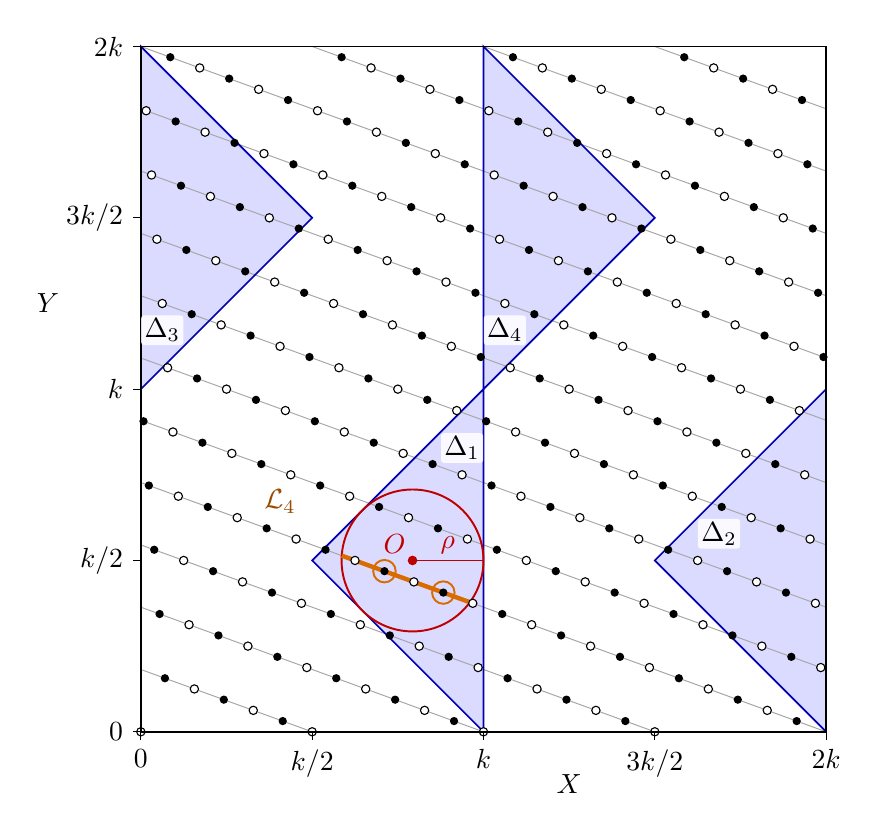
\begin{tikzpicture}[x=0.034cm,y=0.034cm,
  pt/.style={circle,inner sep=0pt,minimum size=3pt},
  lab/.style={fill=white,fill opacity=0.85,text opacity=1,
    inner sep=1.2pt,rounded corners=1pt}]
  % target region R: Delta_1, ..., Delta_4 (k = 128)
  \fill[blue!14] (64,64) -- (128,0) -- (128,128) -- cycle;
  \fill[blue!14] (192,64) -- (256,0) -- (256,128) -- cycle;
  \fill[blue!14] (0,128) -- (0,256) -- (64,192) -- cycle;
  \fill[blue!14] (128,128) -- (128,256) -- (192,192) -- cycle;
  % lattice lines \mathcal L_j = j w + t v, w = (9,20), v = (11,-4)
  \begin{scope}
    \clip (0,0) rectangle (256,256);
    \foreach \j in {0,...,14}
      \draw[black!35,line width=0.35pt]
        ({9*\j-11*10},{20*\j+4*10}) -- ({9*\j+11*21},{20*\j-4*21});
  \end{scope}
  \begin{scope}[blue!70!black,line width=0.6pt]
    \draw (64,64) -- (128,0) -- (128,128) -- cycle;
    \draw (192,64) -- (256,0) -- (256,128) -- cycle;
    \draw (0,128) -- (0,256) -- (64,192) -- cycle;
    \draw (128,128) -- (128,256) -- (192,192) -- cycle;
  \end{scope}
  % incircle D of Delta_1, centre O = (k - rho, k/2), rho = (sqrt2 - 1) k / 2
  \draw[red!75!black,line width=0.7pt] (101.490,64) circle (26.510);
  % chord of \mathcal L_4 across D
  \draw[orange!85!black,line width=1.6pt] (75.04,65.80) -- (122.92,48.39);
  % lattice points (<9d>, <20d>), d = 0, ..., 2k - 1; units are the odd d
  \foreach \d in {0,...,255} {
    \pgfmathtruncatemacro\X{mod(9*\d,256)}
    \pgfmathtruncatemacro\Y{mod(20*\d,256)}
    \ifodd\d
      \node[pt,fill=black] at (\X,\Y) {};
    \else
      \node[pt,draw=black,fill=white,line width=0.4pt] at (\X,\Y) {};
    \fi
  }
  % the two unit points of the chord, d = 67 and d = 41
  \foreach \P in {(91,60),(113,52)}
    \draw[orange!85!black,line width=0.7pt] \P circle (4.2);
  % centre and radius
  \draw[red!75!black,line width=0.6pt] (101.490,64) -- (128,64);
  \fill[red!75!black] (101.490,64) circle (1.8);
  \node[red!75!black,above left=-1pt] at (101.490,64) {$O$};
  \node[red!75!black,above=-1pt] at (114.7,64) {$\rho$};
  % frame and ticks
  \draw[line width=0.6pt] (0,0) rectangle (256,256);
  \foreach \t/\s in {0/0,64/{k/2},128/k,192/{3k/2},256/2k} {
    \draw (\t,0) -- (\t,-3) node[below] {$\s$};
    \draw (0,\t) -- (-3,\t) node[left] {$\s$};
  }
  \node[below=12pt] at (160,0) {$X$};
  \node[left=26pt] at (0,160) {$Y$};
  % labels
  \node[lab] at (120,106) {$\Delta_1$};
  \node[lab] at (216,74) {$\Delta_2$};
  \node[lab] at (8,150) {$\Delta_3$};
  \node[lab] at (136,150) {$\Delta_4$};
  \node[text=orange!60!black,inner sep=0pt] at (52,86) {$\mathcal L_4$};
\end{tikzpicture}
\caption{The geometry of \autoref{lem:lemmaA-region} and
\autoref{prop:lemmaA-band}, drawn to scale for $k=128$ and $(a,e)=(9,20)$.
The square is $[0,2k]^2$ and the shaded triangles are $\Delta_1,\dots,\Delta_4$. The
dots are the $2k$ points $(\langle \nu a\rangle,\langle \nu e\rangle)$ of
$\Lambda$ in the square, filled for the unit points ($\nu$ odd) and open for
the others. A shortest vector is $v=(11,-4)$, of length $l=\sqrt{137}$, and
$w=(a,e)$ has $v\times w=2k$; the grey lines are the lines
$\mathcal L_0,\dots,\mathcal L_{14}$, a distance $2k/l\approx21.9$ apart. The circle is the
incircle of $\Delta_1$, with centre $O$ and radius $\rho$. The line $\mathcal L_4$ passes
within $0.06\,k$ of $O$, and its chord across the disc (thick) contains
the points with $\nu=208,67,182,41$; the two unit points among them (circled)
show that $(9,20)$ has a witness. Here $g=1$ and $n=2$, and both hypotheses of
\autoref{prop:lemmaA-band} hold.}
\label{fig:lemmaA-geometry}
\end{figure}

\begin{lemma}[the target region]
\label{lem:lemmaA-region}
If $\gcd(\nu,2k)=1$ and $(\langle \nu A\rangle,\langle \nu E\rangle)\in R$, then
$\nu$ satisfies \eqref{eq:lemmaA-good}, so $(A,E)$ has a witness.
\end{lemma}

\begin{proof}
Write $X=\langle \nu A\rangle$ and $Y=\langle \nu E\rangle$, so that
$H(\nu A)=H(X)$ and $H(\nu(A\pm E))=H(X\pm Y)$. If $(X,Y)\in \Delta_1$ then
$k-X<Y<X$, so $0<X-Y<2X-k<k$ and $k<X+Y<2X<2k$; hence
$H(X-Y)=1=H(X)$ and $H(X+Y)=0$. If $(X,Y)\in \Delta_3$ then $k+X<Y<2k-X$, so
$X-Y$ lies in $(2X-2k,-k)$, which is $(2X,k)$ modulo $2k$, and $X+Y$ lies in
$(k+2X,2k)$; hence again $H(X-Y)=1=H(X)$ and $H(X+Y)=0$. Finally, replacing
$X$ by $X+k$ adds $k$ to each of $X$ and $X\pm Y$, which reverses all three
values of $H$ and so preserves the pattern $H(X-Y)=H(X)\ne H(X+Y)$. This
covers $\Delta_2$ and $\Delta_4$.
\end{proof}

\subsection{The lattice}

The pairs $(\nu a,\nu e)$ modulo $2k$ are the points of a lattice. It is
simplest to define it by a single congruence:
\[
\Lambda=\{w=(w_1,w_2)\in\Z^2:\ 2k\mid w_1e-w_2a\}.
\]
Since $\gcd(a,e,2k)=1$, fix integers $\xi_1,\xi_2,\xi_3$ with
$\xi_1 a+\xi_2 e+2k\xi_3=1$, and define the \emph{label} of $w\in\Z^2$ as
$\lambda(w)=\xi_1 w_1+\xi_2 w_2$. For $w,w'\in\R^2$ write
$w\times w'=w_1w_2'-w_2w_1'$ and $w\cdot w'$ for the dot product.

\begin{lemma}[labels]
\label{lem:lemmaA-labels}
\begin{enumerate}
\item[(a)] $\Lambda$ is a subgroup of $\Z^2$ containing $2k\Z^2$ and
$(\nu a,\nu e)$ for every $\nu\in\Z$, and every $w\in\Lambda$ satisfies
$w\equiv\lambda(w)\,(a,e)\pmod{2k}$. In particular
$\Lambda=\Z(a,e)+2k\Z^2$, and $\lambda$ is additive.
\item[(b)] If $w,w'\in\Lambda$ then $2k\mid w\times w'$.
\item[(c)] If $w\in\Lambda$, $\gcd(\lambda(w),2k)=1$ and
$(\langle w_1\rangle,\langle w_2\rangle)\in R$, then $(a,e)$ has a witness.
\end{enumerate}
\end{lemma}

\begin{proof}
(a) The first claims are clear. If $w_1e-w_2a=2kc$ then
\[
w_1-\lambda(w)a=w_1(\xi_2 e+2k\xi_3)-\xi_2 aw_2=\xi_2\cdot2kc+2k\xi_3 w_1,
\]
and similarly $w_2-\lambda(w)e=-\xi_1\cdot2kc+2k\xi_3 w_2$.
(b) By (a), $w\times w'\equiv\lambda(w)\lambda(w')\,(a,e)\times(a,e)=0$
modulo $2k$. (c) By (a), $\langle\lambda(w)a\rangle=\langle w_1\rangle$ and
$\langle\lambda(w)e\rangle=\langle w_2\rangle$, so
\autoref{lem:lemmaA-region} applies with $\nu=\lambda(w)$.
\end{proof}

Call $w\in\Lambda$ a \emph{unit point} if $\gcd(\lambda(w),2k)=1$. By
\autoref{lem:lemmaA-labels}(c), the task is to find a unit point of $\Lambda$
in $R+2k\Z^2$. The next lemma collects what a shortest vector of $\Lambda$
provides; part (b) is Hermite's bound in dimension two.

\begin{lemma}[a shortest vector]
\label{lem:lemmaA-frame}
Let $v$ be a nonzero vector of $\Lambda$ of least Euclidean length
$l=|v|$, let $g=\gcd(v_1,v_2)$ and $u=(p,q)=v/g$. Then:
\begin{enumerate}
\item[(a)] there is $w\in\Lambda$ with $v\times w=2k$;
\item[(b)] $3l^4\le16k^2$;
\item[(c)] $g\mid2k$, $gq$ is even, and $mu\notin\Lambda$ for $0<m<g$;
\item[(d)] $g\mid\lambda(v)$, and every common divisor of $\lambda(v)$ and
$2k$ divides $g$;
\item[(e)] $\gcd(\lambda(w),g)=1$ for every $w$ as in (a).
\end{enumerate}
\end{lemma}

\begin{proof}
(a) Write $v_1e-v_2a=2k\varphi$ and $c=\gcd(v_1,v_2,\varphi)$. Then
$v/c\in\Lambda$ is nonzero, so $c=1$ by minimality. Take integers
$\mu_1,\mu_2,\mu_3$ with $\mu_1v_1+\mu_2v_2+\mu_3\varphi=1$ and put
$w=(-2k\mu_2+\mu_3a,\ 2k\mu_1+\mu_3e)$. Then $w\in\Lambda$ (it is
$\mu_3(a,e)$ plus a vector of $2k\Z^2$), and
$v\times w=2k(\mu_1v_1+\mu_2v_2)+\mu_3(v_1e-v_2a)=2k$.

(b) Replacing $w$ by $w+tv$ with $t\in\Z$ does not change $v\times w$, so I
may assume $|v\cdot w|\le l^2/2$. Since $w\ne0$, $|w|\ge l$. Lagrange's
identity $(v\times w)^2+(v\cdot w)^2=|v|^2|w|^2$ gives
$4k^2\ge l^4-l^4/4$.

(c) Let $g'=\gcd(2k,g)=\zeta_12k+\zeta_2g$. Then $g'u=\zeta_1(2ku)+\zeta_2v\in\Lambda$
is nonzero, so $g'|u|\ge l=g|u|$, and $g'=g$; thus $g\mid2k$. If $0<m<g$ then
$mu$ is nonzero and shorter than $v$, so $mu\notin\Lambda$. Finally
$v_2a\equiv v_1e\pmod{2k}$ with $e$ and $2k$ even, so $v_2a$ is even, and
since $a$ is odd, $v_2=gq$ is even.

(d) $\lambda(v)=g(\xi_1 p+\xi_2 q)$. If $c$ divides $\lambda(v)$ and $2k$,
then by \autoref{lem:lemmaA-labels}(a) it divides $v_1$ and $v_2$, hence $g$.

(e) For every $z\in\R^2$, $(v\times w)\,z=(z\times w)\,v+(v\times z)\,w$
(both sides are linear in $z$ and agree at $z=v$ and $z=w$). Take
$z=(a,e)\in\Lambda$: by \autoref{lem:lemmaA-labels}(b) both $z\times w$ and
$v\times z$ are multiples of $2k=v\times w$, so $(a,e)=c_1v+c_2w$ with
$c_1,c_2\in\Z$. Applying the additive map $\lambda$,
$1-2k\xi_3=\xi_1 a+\xi_2 e=c_1\lambda(v)+c_2\lambda(w)$. Since $g$ divides
$2k$ and $\lambda(v)$, it is prime to $\lambda(w)$.
\end{proof}

Replacing $(v,w)$ by $(-v,-w)$ changes none of these properties, so I may
and do assume that $u$ is \emph{normalised}: $p>0$, or $p=0<q$. Eight short
directions never occur.

\begin{lemma}[eight excluded directions]
\label{lem:lemmaA-zero}
With $v=gu$ as in \autoref{lem:lemmaA-frame} and $u=(p,q)$ normalised,
$(g;p,q)$ is none of
\[
(1;1,0),\ (1;1,2),\ (2;0,1),\ (2;1,0),\ (2;1,1),\ (2;1,-1),\ (2;1,-2),\
(4;0,1).
\]
\end{lemma}

\begin{proof}
Each case says that $2k$ divides $g(pe-qa)$, and each contradicts
\eqref{eq:lemmaA-adm}. For $(1;1,0)$: $2k\mid e$, but $0<e<k$.
For $(1;1,2)$: $2k\mid e-2a$ with $|e-2a|<k$, so $e=2a$. For $(2;0,1)$:
$k\mid a$, but $0<a<k$. For $(2;1,0)$: $k\mid e$. For $(2;1,\pm1)$:
$k\mid e\mp a$, which is odd while $k$ is even. For $(2;1,-2)$: $k\mid e+2a$,
but $0<e+2a=x+a<k$. For $(4;0,1)$: $k/2\mid a$, but $0<a<k/2$.
\end{proof}

\subsection{Lattice lines and Jacobsthal's function}
\label{sec:lemmaA-jac}

For $n\ge1$, \emph{Jacobsthal's function} $J(n)$ is the least $m$ such that
every $m$ consecutive integers include one prime to $n$
\citep{Jacobsthal1960a,Jacobsthal1960b,Jacobsthal1960c}. It depends only on
the set of primes dividing $n$, and $J(n')\le J(n)$ whenever every prime
factor of $n'$ divides $n$. Deep asymptotic bounds are known, such as
$J(n)\ll\omega(n)^2\log^2\omega(n)$, with $\omega(n)$ the number of
distinct prime factors of $n$ \citep{Iwaniec1978}, but the elementary bounds
proved below suffice here.

Fix $v=gu$ and $w$ as in \autoref{lem:lemmaA-frame}, and write
$\lambda_v=\lambda(v)$ and $\lambda_w=\lambda(w)$. For $j\in\Z$ let
\[
\mathcal L_j=\{jw+tv:\ t\in\R\}
\]
(see \autoref{fig:lemmaA-geometry}).
Since $v\times(jw+tv)=2kj$, the line $\mathcal L_j$ lies at signed distance
$2kj/l$ from $\mathcal L_0$; consecutive lines are $2k/l$ apart. The points
$jw+iv$ with $i\in\Z$ lie in $\Lambda$, a distance $l$ apart, and their
labels $j\lambda_w+i\lambda_v$ form an arithmetic progression.

\begin{lemma}[unit points on a line]
\label{lem:lemmaA-line}
Let $n\ge1$ divide $2k$, with $\gcd(n,g)=1$ and every prime factor of $2k$
dividing $n$ or $g$ (for instance, $n$ the product of the primes of $2k$
that do not divide $g$). If $\gcd(j,g)=1$, then among any $J(n)$ consecutive
points $jw+iv$ of $\mathcal L_j$ there is a unit point.
\end{lemma}

\begin{proof}
A common divisor of $\lambda_v$ and $n$ divides $2k$, so it divides $g$ by
\autoref{lem:lemmaA-frame}(d), and it is $1$ since $\gcd(n,g)=1$. Choose
$\iota$ with $\iota\lambda_v\equiv1\pmod n$. Then
$j\lambda_w+i\lambda_v\equiv\lambda_v(i+\iota j\lambda_w)\pmod n$, and as $i$ runs
through $J(n)$ consecutive integers so does $i+\iota j\lambda_w$; so for one
of them $j\lambda_w+i\lambda_v$ is prime to $n$. A prime $\ell$ dividing $g$
divides $\lambda_v$ (\autoref{lem:lemmaA-frame}(d)) but neither $j$ nor
$\lambda_w$ (\autoref{lem:lemmaA-frame}(e)), so it does not divide
$j\lambda_w+i\lambda_v$. Every prime of $2k$ divides $n$ or $g$, so this label is
prime to $2k$.
\end{proof}

\begin{lemma}[chords]
\label{lem:lemmaA-chord}
Let $n$ be as in \autoref{lem:lemmaA-line}, $\gcd(j,g)=1$, $\Delta$ one of
$\Delta_1,\dots,\Delta_4$ and $z\in\Z^2$. If $t_0<t_1$, $t_1-t_0>J(n)$ and
$jw+tv\in\Delta+2kz$ for all $t\in(t_0,t_1)$, then $(a,e)$ has a witness.
\end{lemma}

\begin{proof}
The integers $i_0,\dots,i_0+J(n)-1$ with $i_0=\lfloor t_0\rfloor+1$ lie in
$(t_0,t_0+J(n)]\subset(t_0,t_1)$. By \autoref{lem:lemmaA-line} one of the
points $jw+iv$ with such $i$ is a unit point. It lies in $\Delta+2kz$, and since
$\Delta\subset(0,2k)^2$ its residues modulo $2k$ lie in $\Delta\subset R$. Now apply
\autoref{lem:lemmaA-labels}(c).
\end{proof}

\subsection{Two ways to find a chord}

The first way uses a band of lines through the incircle of $\Delta_1$, and works
when the shortest vector is long.

\begin{proposition}[the band]
\label{prop:lemmaA-band}
With $v=gu$ as in \autoref{lem:lemmaA-frame} and $n$ as in
\autoref{lem:lemmaA-line}, suppose that
\[
J(g)<0.102\,l\qquad\text{and}\qquad J(n)\,l<0.3604\,k.
\]
Then $(a,e)$ has a witness.
\end{proposition}

\begin{proof}
Let $D$ be the open disc of radius $\rho$ about the incentre $O$ of $\Delta_1$;
it lies in $\Delta_1$. Put $\tau=(v\times O)/2k$, so that $O$ is at signed
distance $2k\tau/l$ from $\mathcal L_0$. The $J(g)$ consecutive integers
$\lfloor\tau-J(g)/2\rfloor+1,\dots,\lfloor\tau-J(g)/2\rfloor+J(g)$ include
one, $j$, prime to $g$, and every one of them satisfies $|j-\tau|\le J(g)/2$.
So the distance from $O$ to $\mathcal L_j$ is at most
$(2k/l)\,J(g)/2=J(g)k/l<0.102\,k$. The line $\mathcal L_j$ therefore meets $D$
in an open segment of length greater than $2\sqrt{\rho^2-(0.102\,k)^2}$. By
\eqref{eq:lemmaA-rho}, $\rho^2=\tfrac14(3-2\sqrt2)k^2>0.04289\,k^2$, and
$(0.102\,k)^2=0.010404\,k^2$, so the segment is longer than
$2\sqrt{0.03248}\,k>0.3604\,k>J(n)\,l$. In terms of the parameter $t$ of
$\mathcal L_j$ (in which the lattice points sit at the integers) the segment has
length greater than $J(n)$, and it lies in $\Delta_1$.
\autoref{lem:lemmaA-chord} completes the proof.
\end{proof}

The second way handles the short directions. Its key feature is that the
geometry does not depend on $k$, $a$ or $e$ once everything is scaled by
$2k$. Scale the triangles: let $\widehat\Delta_i=\Delta_i/2k$, so that
\begin{align*}
\widehat\Delta_1&=\{(X,Y):\ \tfrac14<X<\tfrac12,\ |Y-\tfrac14|<X-\tfrac14\}, &
\widehat\Delta_2&=\widehat\Delta_1+(\tfrac12,0),\\
\widehat\Delta_3&=\{(X,Y):\ 0<X<\tfrac14,\ |Y-\tfrac34|<\tfrac14-X\}, &
\widehat\Delta_4&=\widehat\Delta_3+(\tfrac12,0).
\end{align*}
For a primitive $u=(p,q)$, an integer $g\ge1$ and $j\in\Z$, consider the
line
\[
\widehat{\mathcal L}_j(g,u)=\Bigl\{\frac{j}{g|u|^2}\,(-q,p)+s\,u:\ s\in\R\Bigr\}.
\]
If $v=gu$ and $w$ are as in \autoref{lem:lemmaA-frame}, then
$(-q,p)\cdot w=u\times w=2k/g$, and decomposing $w$ along $u$ and $(-q,p)$
gives
\begin{equation}
\frac{jw+tv}{2k}=\frac{j}{g|u|^2}\,(-q,p)+\Bigl(s_*+\frac{g}{2k}\,t\Bigr)u,
\qquad s_*=\frac{j\,(u\cdot w)}{2k|u|^2}.
\label{eq:lemmaA-scaled}
\end{equation}
So $\mathcal L_j/2k=\widehat{\mathcal L}_j(g,u)$, and a change of $s$ by $\psi$ is a change of $t$ by
$2k\psi/g$.

\begin{definition}
\label{def:lemmaA-witness}
A \emph{chord witness} for $(g;p,q)$ consists of an integer $j$ with
$\gcd(j,g)=1$, an index $i\in\{1,2,3,4\}$, a vector $z\in\Z^2$ and rationals
$s_0<s_1$ such that the point of $\widehat{\mathcal L}_j(g,u)$ with parameter $s$ lies in
$\widehat\Delta_i+z$ for every $s\in(s_0,s_1)$. Its \emph{length} is
$\psi=s_1-s_0$.
\end{definition}

A chord witness is checked by evaluating finitely many signs. Each
$\widehat\Delta_i+z$ is the intersection of three open half-planes $\{f>0\}$ with
$f$ affine. If, for each of the three functionals, $f\ge0$ at the two points
with parameters $s_0$ and $s_1$ and $f>0$ at one of them, then $f>0$ on the
open segment between them, because along the segment $f$ is a combination
of its two end values with positive weights. These are nine rational sign
conditions.

\begin{proposition}[a tabulated chord]
\label{prop:lemmaA-table}
With $v=gu$ as in \autoref{lem:lemmaA-frame} and $n$ as in
\autoref{lem:lemmaA-line}, suppose $(g;p,q)$ has a chord witness of length
$\psi$ with $2k\psi>J(n)\,g$. Then $(a,e)$ has a witness.
\end{proposition}

\begin{proof}
By \eqref{eq:lemmaA-scaled}, $jw+tv\in\Delta_i+2kz$ for all $t$ in an open
interval of length $2k\psi/g>J(n)$. \autoref{lem:lemmaA-chord} applies.
\end{proof}

When neither proposition applies directly, the lattice can be pinned down
completely. Since $gu\in\Lambda$, the pair $(a,e)$ is, up to a unit, one of
at most $g^2$ explicit pairs.

\begin{lemma}[lattice classes]
\label{lem:lemmaA-class}
Let $v=gu$ be as in \autoref{lem:lemmaA-frame} and $n_0=2k/g$. There are a
unit $\eta$ modulo $2k$ and integers $0\le s,t<g$ (unrelated to the line
parameters above) such that, with
$(A,E)=(p+n_0s,\,q+n_0t)$,
\[
\eta\,(a,e)\equiv(A,E)\pmod{2k}.
\]
Moreover $\gcd(A,E,2k)=1$, and $2k\nmid m(pE-qA)$ for $0<m<g$. In
particular, if $(A,E)$ has a witness then so does $(a,e)$.
\end{lemma}

\begin{proof}
By \autoref{lem:lemmaA-frame}(d), $\lambda_v=\lambda(v)=g\lambda^*$, and
$\gcd(\lambda^*,n_0)=1$: if $c$ divides both then $gc$ divides $2k$ and
$\lambda_v$, hence $g$, so $c=1$. By \autoref{lem:lemmaA-labels}(a),
$g(p,q)=v\equiv g\lambda^*(a,e)\pmod{2k}$, so
$\lambda^*(a,e)\equiv(p,q)\pmod{n_0}$. Every unit modulo $n_0$ lifts to a
unit modulo $2k$: take $\eta=\lambda^*+n_0r$, with $r$ the product of the
primes of $2k$ that divide neither $n_0$ nor $\lambda^*$. Indeed, let $\ell$ be
a prime dividing $2k$. If $\ell\mid n_0$, then $\eta\equiv\lambda^*\not\equiv0
\pmod\ell$, as $\gcd(\lambda^*,n_0)=1$. If $\ell\nmid n_0$ and
$\ell\mid\lambda^*$, then $\ell\nmid r$, and $\eta\equiv n_0r\not\equiv0$. If
$\ell$ divides neither, then $\ell\mid r$, and $\eta\equiv\lambda^*\not\equiv0$. Then
$\eta a=p+n_0K_1$ and $\eta e=q+n_0K_2$ for some integers $K_1,K_2$, and
with $s,t$ the residues of $K_1,K_2$ modulo $g$ one gets
$\eta(a,e)\equiv(A,E)\pmod{n_0g}$, as claimed.

If $c$ divides $A$, $E$ and $2k$, it divides $\eta a$ and $\eta e$, hence
$\eta(\xi_1 a+\xi_2 e+2k\xi_3)=\eta$, and $c=1$. If $2k\mid m(pE-qA)$, then
$2k\mid m\eta(pe-qa)$, so $2k\mid m(pe-qa)$, that is $mu\in\Lambda$; this is
impossible for $0<m<g$ by \autoref{lem:lemmaA-frame}(c). For the last
statement, if a unit $\nu$ satisfies \eqref{eq:lemmaA-good} for $(A,E)$, then
$\nu\eta$ is a unit, and it satisfies \eqref{eq:lemmaA-good} for $(a,e)$ because
$\nu\eta(a,e)\equiv \nu(A,E)\pmod{2k}$.
\end{proof}

The two conditions on $(A,E)$ in \autoref{lem:lemmaA-class} are used in
reverse: a class $(s,t)$ for which $\gcd(A,E,2k)>1$, or for which
$2k\mid m(pE-qA)$ for some $0<m<g$, cannot arise from an admissible
$(a,e)$ with shortest vector $gu$, and needs no witness.

\subsection{The chord table and orders above 2730}
\label{sec:lemmaA-tail}

The two propositions of the last subsection settle every large order. The band
(\autoref{prop:lemmaA-band}) needs a long shortest vector, and the short ones
are covered once and for all by a table of chords.

Let $\mathcal V$ be the set of triples $(g;p,q)$ with $g\ge1$, $(p,q)$
primitive and normalised, $gq$ even, $g^2(p^2+q^2)\le6400$, and $(g;p,q)$
not one of the eight triples of \autoref{lem:lemmaA-zero}. By
\autoref{lem:lemmaA-frame}(c) and \autoref{lem:lemmaA-zero}, a normalised
shortest vector $v=gu$ of $\Lambda$ with $l\le80$ gives a triple
$(g;p,q)\in\mathcal V$ with $g\mid2k$. The following finite computation is
the first part of the certificate for \autoref{thm:lemmaA};
the other two parts, (C2) and (C3), are in \autoref{app:lemmaA-finite}.
\begin{enumerate}
\item[(C1)] \emph{The chord table.} For each of the $5012$ triples of
$\mathcal V$ a chord witness is given and its nine sign conditions are
verified (after clearing denominators). That the table lists exactly the
elements of $\mathcal V$ is checked by enumerating all $g\le80$ and all
$(p,q)$ with $0\le p\le80/g$ and $|q|\le80/g$. Only lower bounds on chord
lengths are used, so the witnesses need not be the longest chords. Every entry has
\begin{equation}
g\le339.8\,\psi,
\label{eq:lemmaA-ratio}
\end{equation}
where $\psi$ is the length of its chord witness; the extreme entry is
$(76;1,0)$, with $\psi=17/76$ and $g/\psi=339.76\ldots$.
\end{enumerate}

Say that an even order $k$ satisfies the \emph{tail condition} with bound $m$ if
\begin{equation}
17.8\,m^2\le k\qquad\text{and}\qquad169.9\,m<k ,
\label{eq:lemmaA-tailcond}
\end{equation}
that is, $178\,m^2\le10k$ and $1699\,m<10k$ in integers. The first inequality
is what the band (\autoref{prop:lemmaA-band}) needs, $J(n)\,l<0.3604\,k$,
after Hermite's bound $l^2\le4k/\sqrt3$; the second is what a tabulated chord
(\autoref{prop:lemmaA-table}) needs, $2k\psi>J(n)\,g$, after
\eqref{eq:lemmaA-ratio}. The bounds on Jacobsthal's function used below are
proved in \autoref{app:lemmaA-jacbounds} (\autoref{cor:lemmaA-jac}).

\begin{proposition}
\label{prop:lemmaA-tail}
Let $k$ be even and satisfy the tail condition
\eqref{eq:lemmaA-tailcond} with bound $m=J(2k)$. Then \autoref{thm:lemmaA}
holds at the order $k$. The tail condition with $m=J(2k)$ holds for every
even $k>2730$.
\end{proposition}

\begin{proof}
For the last statement, write $J=J(2k)$. By \autoref{cor:lemmaA-jac}(a),
$17.8\,J^2\le k$. If $J\ge10$ this gives $169.9\,J<178\,J\le17.8\,J^2\le k$,
and if $J\le9$ then $169.9\,J<1530<k$.

Now let $v=gu$ be a normalised shortest vector of $\Lambda$, and $n$ the
product of the primes of $2k$ not dividing $g$, so that $n$ satisfies the
conditions of \autoref{lem:lemmaA-line} and $J(n)\le J$. By hypothesis,
$17.8\,J^2\le k$ and $k>169.9\,J$.

\emph{Short vectors, $l^2\le6400$.} Then $(g;p,q)\in\mathcal V$ by
\autoref{lem:lemmaA-frame}(c) and \autoref{lem:lemmaA-zero}, and
\eqref{eq:lemmaA-ratio} gives $2k\psi\ge kg/169.9>Jg\ge J(n)g$, so
\autoref{prop:lemmaA-table} applies.

\emph{Long vectors, $l>80$.} By \autoref{cor:lemmaA-jac}(b), either
$J(g)\le8<0.102\cdot80<0.102\,l$, or $J(g)<0.102\,g\le0.102\,l$. By
\autoref{lem:lemmaA-frame}(b), $l^2\le4k/\sqrt3$, so
\[
J(n)^2l^2\le\frac{k}{17.8}\cdot\frac{4k}{\sqrt3}<0.12975\,k^2,
\]
and $J(n)\,l<0.36021\,k$. So \autoref{prop:lemmaA-band} applies.
\end{proof}

\subsection{Orders with at most two odd primes}
\label{sec:lemmaA-twoprime}

When $k$ has at most two odd prime factors, \autoref{thm:lemmaA} has a direct
proof, with no lattice. It covers $1193$ of the $1320$ orders
$92\le k\le2730$, so that the finite certificate is needed only at the $127$
orders with three or more odd prime factors. The idea is that one term of the
progression is then a unit; normalising it to $1$ leaves a one-parameter
problem, which explicitly located multipliers solve. Throughout, if $c$ is a
unit and $\nu$ satisfies \eqref{eq:lemmaA-good} for the pair $(cA,cE)$, then
$\nu c$ satisfies it for $(A,E)$; so $(A,E)$ has a witness as soon as
$(cA,cE)$ does.

\begin{lemma}[two normal forms]
\label{lem:lemmaA-normal}
Let $k$ be even.
\begin{enumerate}
\item[(a)] If $m$ is a unit with $0<m<k$ and $k+m<\langle mD\rangle<2k-m$,
then $m$ satisfies \eqref{eq:lemmaA-good} for the pair $(1,D)$.
\item[(b)] If $\nu$ is a unit with $0<\nu<k$, $\langle\nu A\rangle=r<k$ and
$\langle2r-\nu\rangle\ge k$, then $\nu$ satisfies \eqref{eq:lemmaA-good} for the
pair $(A,A-1)$.
\end{enumerate}
\end{lemma}

\begin{proof}
(a) Write $Y=\langle mD\rangle$. Then $H(m)=1$. Next, $m(1+D)\equiv m+Y$ with
$k+2m<m+Y<2k$, so $H(m(1+D))=0$; and $m(1-D)\equiv m-Y+2k$ with
$2m<m-Y+2k<k$, so $H(m(1-D))=1$.
(b) Here $H(\nu)=1=H(\nu A)$, and $\nu(2A-1)\equiv2r-\nu$, so
$H(\nu(2A-1))=0$.
\end{proof}

The multipliers for a unit middle term come in \emph{chains}. A chain is a
list $(m_1,i_1),\dots,(m_N,i_N)$ of odd multipliers $m_j$ and integers
$i_j\ge0$, with a threshold $K$, such that
\begin{equation}
\frac{2i_1+1}{m_1}+\frac1K\le\frac18,\qquad
\frac{2i_{j+1}+1}{m_{j+1}}+\frac1K<\frac{2i_j+2}{m_j}-\frac1K,\qquad
\frac{2i_N+2}{m_N}-\frac1K>\frac12 ,
\label{eq:lemmaA-chain}
\end{equation}
the middle condition for $j=1,\dots,N-1$. The pair $(m_j,i_j)$ serves when
$D/k$ lies roughly in the interval $\bigl((2i_j+1)/m_j,\,(2i_j+2)/m_j\bigr)$,
where $m_jD$ falls in the window $\bigl((2i_j+1)k,\,(2i_j+2)k\bigr)$; the three
conditions say that, with a margin $1/K$, these intervals overlap and together
cover $[1/8,1/2]$. \autoref{tab:lemmaA-chains} lists
ten chains, one for each pattern of small primes dividing $k$; their
conditions \eqref{eq:lemmaA-chain} are checked in exact rational arithmetic.

\begin{table}
\centering
\small
\begin{tabular}{llr}
case & chain $m_1^{i_1}\,m_2^{i_2}\cdots$ & $K$\\\hline
$3,5\nmid k$ & $9^0\,5^0\,3^0$ & $92$\\
$3\mid k$; $5,7,11,13,19\nmid k$ & $11^0\,7^0\,5^0\,19^3\,13^2\,7^1$ & $96$\\
$5\mid k$; $3,7,11\nmid k$ & $9^0\,7^0\,27^3\,11^1\,3^0$ & $100$\\
$15\mid k$ & $11^0\,7^0\,19^2\,11^1\,49^8\,43^7\,31^5\,19^3\,13^2\,7^1$ & $120$\\
$21\mid k$ & $11^0\,19^1\,17^1\,5^0\,19^3\,23^4\,17^3\,11^2$ & $126$\\
$33\mid k$ & $13^0\,25^1\,7^0\,5^0\,13^2\,7^1$ & $132$\\
$39\mid k$ & $11^0\,19^1\,17^1\,5^0\,19^3\,23^4\,17^3\,11^2$ & $156$\\
$57\mid k$ & $11^0\,7^0\,5^0\,29^5\,13^2\,7^1$ & $114$\\
$35\mid k$ & $9^0\,17^1\,23^2\,13^1\,11^1\,3^0$ & $140$\\
$55\mid k$ & $9^0\,7^0\,19^2\,17^2\,3^0$ & $110$
\end{tabular}
\caption{The chains used in the proof of \autoref{prop:lemmaA-twoprime}, for
even $k\ge92$ with at most two odd prime factors; $m^i$ stands for the pair
$(m,i)$. In each case $K$ is the least such order, so $k\ge K$, and every
multiplier is a unit.}
\label{tab:lemmaA-chains}
\end{table}

\begin{proposition}[two odd primes]
\label{prop:lemmaA-twoprime}
Let $k\ge92$ be even, with at most two odd prime factors. Then every
admissible triple $(k;a,x)$ has a witness.
\end{proposition}

\begin{proof}
The units modulo $2k$ are the odd integers prime to the odd primes of $k$, of
which there are at most two. So if three odd integers are such that no prime
factor of $k$ divides two of them, one of them is a unit. Write $e=x-a$, so
that \eqref{eq:lemmaA-adm} holds. An odd prime of $k$ dividing two of $a-e$,
$a$, $a+e$ divides $a$ and $e$, which \eqref{eq:lemmaA-adm} excludes, so one of
these three is a unit.

\emph{The case where $a$ is a unit.} Let $\bar a$ be its inverse modulo $2k$
and $D=\langle\bar ae\rangle$, which is even. It suffices to find a witness for
$(1,D)$. Since $aD\equiv e$, the values $D=0,2,k-2,k,k+2,2k-2$ would give
$e\equiv0,2a,k-2a,k,k+2a,-2a\pmod{2k}$, which \eqref{eq:lemmaA-adm} excludes
(as $0<e$, $e\ne2a$ and $e+2a<k$). By \autoref{lem:lemmaA-normal}(a) it
suffices to find a unit $m$ with $0<m<k$ and
\begin{equation}
(2i+1)k+m<mD<(2i+2)k-m\qquad\text{for some integer } i .
\label{eq:lemmaA-window}
\end{equation}
If $k<D<2k$, then $m=1$ works, with $i=0$. For odd $m$, if $m$ satisfies
\eqref{eq:lemmaA-window} for $k-D$ with some $i$, then it satisfies it for $D$
with $i$ replaced by $(m-3)/2-i$, since $mD=mk-m(k-D)$. So it may be assumed
that $4\le D\le k/2$.

If $8D\le k$, every $m$ in the interval $I=\bigl(k/(D-1),\,2k/(D+1)\bigr)$
has $m(D-1)>k$ and $m(D+1)<2k$, which is \eqref{eq:lemmaA-window} with $i=0$,
and $m<2k/5$. The length of $I$ is $k(D-3)/(D^2-1)$, which exceeds $6$: for
$D\le11$ because $k\ge92$, and for $D\ge12$ because $k\ge8D$ and
$8D(D-3)-6(D^2-1)=2D(D-12)+6>0$. So $I$ contains three consecutive odd
integers. Their pairwise differences are $2$ and $4$, so no odd prime divides
two of them, and one of them is a unit.

If $8D>k$, take the chain of \autoref{tab:lemmaA-chains} for the case of $k$;
the cases are exhaustive, and in each the multipliers are units, because $k$
has at most two odd primes. The first multiplier satisfies the left inequality
of \eqref{eq:lemmaA-window}, as $m_1D>m_1k/8\ge(2i_1+1)k+m_1k/K\ge(2i_1+1)k+m_1$,
since $k\ge K$. If $m_j$
satisfies the left inequality but not the right one, then
$D/k\ge(2i_j+2)/m_j-1/k$, and \eqref{eq:lemmaA-chain} gives the left
inequality for $m_{j+1}$. The right inequality cannot fail for $m_N$, as
$D/k\le1/2$. So some $m_j$ satisfies \eqref{eq:lemmaA-window}.

\emph{The case where $a-e$ is a unit.} Let $y=2a-x=a-e$, $\bar y$ its inverse
and $A=\langle\bar ya\rangle$. Then $\bar ye\equiv A-1$, so it suffices to find
a witness for $(A,A-1)$. It may be assumed that $a$ is not a unit. Let
$f=\gcd(A,2k)=\gcd(a,k)$. It is odd and $1<f\le a<k/2$, so $k/f$ is even and
at least $4$. Write $A=fA_0$ and $M=2k/f$, so that $A_0$ is prime to $M$, and let
$\nu_0\in(0,M)$ be its inverse modulo $M$. Every $\nu\equiv c\nu_0\pmod M$ has
$\nu A\equiv fc\pmod{2k}$. The \emph{lifts} $\nu\equiv\nu_0\pmod M$ are odd and
prime to $M$, and by \autoref{lem:lemmaA-normal}(b) with $r=f$, every lift
that is a unit and lies in $(2f,k)$ is a witness, since
$\langle2f-\nu\rangle=2k+2f-\nu\ge k$. A prime of $k$ dividing a lift does not
divide $M$, so it divides $f$.

If $f\ge15$, then $2f+3M\le k$, so the interval $(2f,k)$ contains three
lifts $\nu$, $\nu+M$ and $\nu+2M$; their pairwise differences divide $2M$, to
which $\nu$ is prime, so one of them is a unit. If $5\le f\le13$, then $f$ is
a power of a single prime $\ell$, and $2f+2M\le k$ (using $k\ge92$ when
$f\in\{5,7\}$), so $(2f,k)$ contains two lifts $\nu$ and $\nu+M$; a lift that
is not a unit is divisible by $\ell$, and $\ell$ cannot divide both, as $\nu$
is prime to $M$. If $f=3$ and $9\mid k$, then $3\mid M$, so every lift is prime
to $3$ and a unit, and $2f+M\le k$ gives one in $(6,k)$.

There remains $f=3$ with $3\nmid M$, so that $k=3q$ with $q$ even, $3\nmid q$
and $q\ge32$, and $M=2q$. A number prime to $M$ is then a unit when it is
prime to $3$, and $\nu_0$ is odd. If $6<\nu_0<q$, the lifts $\nu_0$ and
$\nu_0+M$ both lie in $(6,k)$, and one is prime to $3$. If $\nu_0>q$ and
$3\nmid\nu_0$, take $\nu=\nu_0$. If $\nu_0>q$ and $3\mid\nu_0$, take $c=q-3$
and $\nu$ the residue of $c\nu_0$ modulo $M$, so that $\nu A\equiv3c=k-9$.
Here $\nu$ is prime to $M$, since a common prime factor of $q-3$ and $q$
divides $3$. As $\nu_0$ is odd, $q\nu_0\equiv q\pmod M$, so
$\nu\equiv q-3\nu_0$, and as $q<\nu_0<2q$, $\nu$ is $5q-3\nu_0$ or
$7q-3\nu_0$, which is prime to $3$. Then
$\langle2(k-9)-\nu\rangle=2k-18-\nu\ge k$, since $\nu<M\le k-18$. Finally, if
$\nu_0<6$, the lift $\nu_0+M$ lies in $(6,k)$, and is a witness unless it is
divisible by $3$. In that case $\nu_0\in\{1,5\}$ and $q\equiv\nu_0\pmod3$. Let $s=5$ if $5\nmid k$; if
$5\mid k$, then $5\mid M$, so $\nu_0=1$, and let $s=11$, which does not divide
$k$, as $3$ and $5$ do. Take $c=q-s$ and $\nu=q-s\nu_0\equiv c\nu_0\pmod M$,
so that $\nu A\equiv3c=k-3s$. A common prime factor of $\nu$ and $q$ divides
$s\nu_0$, and none does; $\nu\equiv\nu_0(1-s)\not\equiv0\pmod3$; and
$2k-6s-\nu\ge k$, since $2q\ge64\ge s(6-\nu_0)$. In each case
\autoref{lem:lemmaA-normal}(b) gives the witness.

\emph{The case where $a+e$ is a unit.} Suppose finally that neither $a$ nor
$a-e$ is a unit, so that $y'=a+e=x$ is. With $\bar y'$ its inverse and
$A'=\langle\bar y'a\rangle$, $\bar y'e\equiv1-A'$, so it suffices to find a
witness for $(A',1-A')$, whose progression is $2A'-1$, $A'$, $1$. Let
$A=A'+k$. For a unit $\nu$, which is odd, $H(\nu A)=1-H(\nu A')$ and
$\nu(2A-1)\equiv\nu(2A'-1)$, so $\nu$ satisfies \eqref{eq:lemmaA-good} for
$(A,A-1)$ exactly when it does for $(A',1-A')$. Since $A'$ is odd and $k$
even, $\gcd(A,2k)=\gcd(A',2k)=\gcd(a,k)$, and the previous case, applied to
$A$, gives the witness.
\end{proof}

\begin{proof}[Proof of \autoref{thm:lemmaA}]
If $k$ has at most two odd prime factors, \autoref{prop:lemmaA-twoprime}
applies. Otherwise, if $k>2730$, \autoref{prop:lemmaA-tail} applies, and if
$k\le2730$, $k$ is one of the $127$ orders of the finite certificate of
\autoref{prop:lemmaA-finite} in \autoref{app:lemmaA-finite}.
\end{proof}

For $92\le k\le2730$ the theorem can also be confirmed directly, independently
of the certificate: a direct search over the units $\nu$ modulo $2k$ finds a
witness for each of the $100\,435\,222$ admissible triples $(k;a,x)$ in this
range.

\section{Proof of the main theorem}
\label{sec:assembly}

By \autoref{cor:red-primitive} it is
enough to show the following: if an equation \eqref{eq:familya} is
globally periodic, its support $S$ is primitive and its coefficients
satisfy $c_j=c_{k-j}$, then its normalised data is of known type
(\autoref{def:red-known}). So let such an equation be given. Since
$c_j=c_{k-j}$, its support is palindromic.

\emph{$|S|\le2$.} By the case analysis at the start of \autoref{sec:small},
either $S=\emptyset$, which is case (K1); or $k=2$ and $S=\{1\}$, where
\autoref{thm:order2} gives case (K2); or $k=3$ and $S=\{1,2\}$, where
\autoref{thm:order3} gives case (K3); or \autoref{thm:twoterm} shows that the
equation is not globally periodic, a contradiction.

\emph{$|S|\ge3$.} I show that no such equation is globally periodic,
which leaves only the three cases above. If $S$ is the full support
$\{1,\dots,k-1\}$, then $k\ge4$ and \autoref{thm:fullsupport} applies. So
suppose $S$ is not the full support. If $k$ is odd, \autoref{thm:oddk}
applies. If $k=6$ and $S=\{1,3,5\}$, \autoref{prop:order6cert} applies.
Otherwise $k$ is even and $(k,S)\ne(6,\{1,3,5\})$, and $S$ carries a
$\sigma$-bump: by \autoref{thm:notallodd} if $S$ has an even element, and
by \autoref{thm:alloddall} if every element of $S$ is odd. In either case
\autoref{thm:sigmabump} shows that no equation with support $S$ is
globally periodic.

So every globally periodic equation \eqref{eq:familya} with primitive support and
palindromic coefficients has normalised data of known type. By
\autoref{cor:red-primitive}, a globally periodic equation \eqref{eq:family} is
therefore the shift or has the coefficients listed in \autoref{lem:red-members},
and these are exactly the equations listed in \autoref{thm:main}. This completes
the proof of \autoref{thm:main}. \qed

The argument for supports with three or more elements never uses the
coefficients, and it therefore also proves a statement about the min-plus
recursion alone, extending the result of \citet{CsornyeiLaczkovich2001} for the
full support (\autoref{sec:fullsupport}).

\begin{corollary}[the min-plus map is not periodic]
\label{cor:trop-nonperiodic}
Let $S\subseteq\{1,\dots,k-1\}$ be palindromic with $|S|\ge3$, and let
$\theta\in\{0,1\}$. Then no power of the min-plus map $T$ of
\autoref{def:trop-minplus} is the identity: for every $p\ge1$ there is an
integer window $w\in\Z^k$ with $T^{\,p}(w)\ne w$.
\end{corollary}

\begin{proof}
Suppose first that $S$ is primitive. The proof of \autoref{thm:main} above
provides an integer solution $e$ of the min-plus recursion \eqref{eq:trop-rec}
for $(k,S,\theta)$ that carries an unbounded integer tangent solution $d$: for
the full support by \autoref{lem:fs-carrier} and \autoref{lem:fs-ray}; at
odd order by the construction in the proof of \autoref{prop:odd-second}, with
the solutions of the reduced recursion given in the proof of
\autoref{thm:odd-nondil}, or by a $\sigma$-bump; for $\{1,3,5\}$ at order $6$ by
the construction in the proof of \autoref{prop:trop-cert}; and otherwise by a
$\sigma$-bump and \autoref{lem:trop-bumptangent}. None of these constructions
involves the coefficients $c_j$, so \autoref{thm:tangent}(ii) applies.

If $S$ is not primitive, let $\ell=\gcd(S\cup\{k\})$, and let $S'$ and
$k'$ be as in \autoref{lem:unfold}; then $S'$ is primitive and palindromic,
with $|S'|=|S|\ge3$. As in the proof of \autoref{lem:unfold}(ii), if $z$ is an
integer solution of the min-plus recursion for $(k',S',\theta)$, then
$x_n=z_{\lfloor n/\ell\rfloor}$ is one for $(k,S,\theta)$. So if $T^{\,p}=\id$,
every such $x$ is $p$-periodic, and $z_{m+p}=x_{m\ell+p\ell}=x_{m\ell}=z_m$;
that is, the min-plus map for $(k',S',\theta)$ has $p$-th power the identity,
against the primitive case.
\end{proof}

Since $\Z^k\subset\R^k$, the min-plus map is not periodic on $\R^k$ either.
Note that the corollary asserts only that $T$ is not periodic. Unlike the
theorems of \citeauthor{CsornyeiLaczkovich2001} for the full support, it does
not exhibit a single non-periodic orbit, since the window $w$ depends on $p$. The
hypothesis $|S|\ge3$ cannot simply be dropped: with $\theta=1$ the min-plus
maps for $S=\{1\}$ at order $2$ and $S=\{1,2\}$ at order $3$ are periodic,
with periods $5$ and $8$ (\autoref{sec:small}).

The corollary leaves the two-term supports $\{j,k-j\}$ open, since the proof
of \autoref{thm:main} settles them with the linearisation. For $k=4$ and
$S=\{1,3\}$ the tangent certificates (\autoref{def:trop-cert}) with
$E=(-1,-1,-1,-1)$ and
\begin{align*}
\theta=1:&\quad q=11,\ V=(-1,-1,0,-1),\ W=(0,0,1,1),\
(w_t)=1,1,1,3,0,1,3,3,3,3,1,\\
\theta=0:&\quad q=66,\ V=(-1,-1,0,0),\ W=(4,0,0,0),\
(w_t)=1^63^51^63^51^63^61^53^61^53^61^53^5,
\end{align*}
($1^6$ stands for six consecutive entries $1$) are valid along the
$11$-periodic solution with window $E$, so, by the argument above, no power
of the min-plus map for $(4,\{1,3\},\theta)$ is the identity, for either
$\theta$. Whether this holds for every two-term support other than $\{m,2m\}$ at order
$3m$ with $\theta=1$, where the map is periodic by unfolding the order-$3$
case, and which
non-palindromic supports have a periodic min-plus map, I leave open.


\section*{Acknowledgements}

This proof was AI-generated with fairly limited input from the human author. 
The models used were Claude Opus 5.5 and Fable 5.1.

\appendix
\section{The finite range of the progression theorem}
\label{app:lemmaA-finite}

This appendix completes the proof of \autoref{thm:lemmaA}. It gives the
certificate for the $127$ orders $92\le k\le2730$ with at least three odd
prime factors, the only ones not covered by \autoref{prop:lemmaA-twoprime}
or \autoref{prop:lemmaA-tail}, and proves the two bounds on
Jacobsthal's function used in \autoref{sec:lemmaA-tail} for the orders above
$2730$. The notation is that of \autoref{sec:lemmaA}.

\subsection{The orders up to 2730 with three or more odd primes}

By \autoref{lem:lemmaA-frame}(b), (c) and \autoref{lem:lemmaA-zero}, the
normalised shortest vector of $\Lambda$ at an order $k\le2730$ gives a triple
in $\mathcal V$ with $g\mid2k$ and $3l^4\le16k^2$: indeed
$l^4\le16\cdot2730^2/3$ gives $l^2\le6304<6400$, so $l\le80$. Besides the chord table (C1) of
\autoref{sec:lemmaA-tail}, the finite certificate has two more parts.
\begin{enumerate}
\item[(C2)] \emph{Jacobsthal values.} A list of $224$ pairs $(n,m)$ with
$J(n)\le m$. Each is checked over one period: for every residue $y$ modulo
$n$ some $0\le i<m$ has $\gcd(y+i,n)=1$.
\item[(C3)] \emph{The per-order certificate.} For each of the $127$ even
$k$ with $92\le k\le2730$ that have at least three odd prime factors, either
(C2) contains a pair $(n,m)$ with $n$ the product of the primes of $2k$ such
that $k$ satisfies the tail condition \eqref{eq:lemmaA-tailcond} with bound
$m$ (the \emph{tail alternative}), or, for each $(g;p,q)\in\mathcal V$ with $g\mid2k$ and
$3\bigl(g^2(p^2+q^2)\bigr)^2\le16k^2$, one of the following is verified:
\begin{enumerate}
\item[(i)] a pair $(n,m)$ from (C2) with $n\mid2k$, $\gcd(n,g)=1$, every
prime of $2k$ dividing $ng$, and $2k\psi>mg$, where $\psi$ is the length
of the chord witness in (C1); or
\item[(ii)] for each of the $g^2$ pairs $0\le s,t<g$, with
$(A,E)=(p+\tfrac{2k}{g}s,\,q+\tfrac{2k}{g}t)$: a unit $\nu<100$
satisfying \eqref{eq:lemmaA-good}, or $\gcd(A,E,2k)>1$, or an
$m$ with $0<m<g$ and $2k\mid m(pE-qA)$.
\end{enumerate}
\end{enumerate}
The tail alternative of (C3) holds at $65$ of these $127$ orders, and
alternative (ii) is needed only at $18$ orders, all at most $924$.

\begin{proposition}
\label{prop:lemmaA-finite}
\autoref{thm:lemmaA} holds at the $127$ even orders $92\le k\le2730$ with at
least three odd prime factors.
\end{proposition}

\begin{proof}
If the tail alternative of (C3) holds, then $J(2k)=J(n)\le m$ and $k$
satisfies the tail condition with bound $m$, hence with bound $J(2k)$, and
\autoref{prop:lemmaA-tail} applies. Otherwise, let $v=gu$ be a normalised shortest vector of
$\Lambda$. As noted above, $(g;p,q)\in\mathcal V$, $g\mid2k$ and
$3l^4\le16k^2$, so (C3) applies to it. In case (i), $J(n)\le m$ and $2k\psi>J(n)g$, and
\autoref{prop:lemmaA-table} shows that $(a,e)$ has a witness; the conditions on $n$
are those of \autoref{lem:lemmaA-line}. In case (ii), let $(s,t)$ be the
class given by \autoref{lem:lemmaA-class}. Its two exclusions are ruled out
by that lemma, so the certificate gives a unit $\nu$ showing that $(A,E)$ has a
witness, and then so does $(a,e)$, by \autoref{lem:lemmaA-class}.
\end{proof}


\subsection{Elementary bounds on Jacobsthal's function}
\label{app:lemmaA-jacbounds}

This subsection proves \autoref{cor:lemmaA-jac}, the two inequalities for
Jacobsthal's function used in \autoref{prop:lemmaA-tail}, by a union bound and
a progression trick.

\begin{lemma}
\label{lem:lemmaA-jactools}
\begin{enumerate}
\item[(a)] Suppose every $m$ consecutive integers include at least $c$ that
are prime to $N$, and $\mathcal T$ is a finite set of primes with
$\sum_{p\in\mathcal T}\lceil m/p\rceil<c$. Then $J(n)\le m$ for every $n\ge1$
whose prime factors divide $N$ or lie in $\mathcal T$.
\item[(b)] If $\gcd(f,N)=1$ then $J(fN)\le f\,J(N)$.
\end{enumerate}
\end{lemma}

\begin{proof}
(a) Among $m$ consecutive integers at most $\lceil m/p\rceil$ are multiples
of $p$. So fewer than $c$ of them are divisible by a prime of $\mathcal T$,
and one of the $c$ integers prime to $N$ escapes; it is prime to $n$.

(b) Given a run $y,y+1,\dots,y+fJ(N)-1$, choose $0\le r<f$ with
$y+r\equiv1\pmod f$, and consider $y_i=y+r+fi$ for $0\le i<J(N)$, all in the
run. Each $y_i$ is prime to $f$. With $f'$ an inverse of $f$ modulo $N$,
$f'y_i\equiv f'(y+r)+i\pmod N$ runs through $J(N)$ consecutive integers, so
some $y_i$ is prime to $N$, hence to $fN$.
\end{proof}

Let $\varpi_1<\varpi_2<\dots<\varpi_8$ be the primes $17,19,23,29,31,37,41,43$ and
$\Pi_r=\varpi_1\cdots \varpi_r$ (with $\Pi_0=1$), and recall that $\omega(n)$ is the
number of distinct prime factors of $n$.

\begin{lemma}[at most eight prime factors]
\label{lem:lemmaA-pattern}
Let $n\ge1$ with $\omega(n)\le8$. Let $B$ be the product of the primes
$p\le13$ dividing $n$, and $r$ the number of primes $p>13$ dividing $n$.
Then $B\Pi_r\le n$, and there is an $m$ with $J(n)\le m$ such that
\begin{enumerate}
\item[(i)] if $B$ is even, $178\,m^2\le10\max\bigl(B\Pi_r,\
B(\lfloor2730/B\rfloor+1)\bigr)$;
\item[(ii)] $m\le8$, or $1000\,m<102\,B\Pi_r$.
\end{enumerate}
\end{lemma}

The maximum in (i) is the better of two lower bounds for an order $k$ to
which the lemma will be applied: $k\ge B\Pi_r$, and, as $k$ is a multiple
of $B$ above $2730$, $k\ge B(\lfloor2730/B\rfloor+1)$. So (i) gives the first
inequality of the tail condition, and (ii) gives $J(g)\le8$ or
$J(g)<0.102\,g$, as needed for the band.

\begin{proof}
The $i$-th smallest prime above $13$ is $\varpi_i$, so the primes
$p_1<\dots<p_r$ of $n$ above $13$ satisfy $p_i\ge \varpi_i$. Hence
$n\ge B\,p_1\cdots p_r\ge B\Pi_r$, and
$\sum_i\lceil m/p_i\rceil\le\sum_i\lceil m/\varpi_i\rceil$ for every $m$.

The rest is a finite table. For each of the $64$ sets $\mathcal P$ of primes
$\le13$, with product $B$, and each $r$ with $0\le r\le8-|\mathcal P|$, there is an
entry; this gives $384$ pairs $(B,r)$. For each the table supplies integers
$m$ and $c$ such that
\begin{enumerate}
\item[(P1)] every $m$ consecutive integers include at least $c$ that are
prime to $B$;
\item[(P2)] $\sum_{i=1}^r\lceil m/\varpi_i\rceil<c$;
\item[(P3)] (i) and (ii) hold for this $m$.
\end{enumerate}
Condition (P1) is checked by sliding a window of length $m$ over one period
$\{0,\dots,B-1\}$ of the starting point; (P2) and (P3) are arithmetic. The
largest $m$ needed is $84$. Given the table, (P1), (P2)
and the inequality above give exactly the situation of
\autoref{lem:lemmaA-jactools}(a), with $N=B$ and $\mathcal T$ the primes of
$n$ above $13$, so $J(n)\le m$.
\end{proof}

\begin{lemma}[at least nine prime factors]
\label{lem:lemmaA-crude}
Let $n$ have $\omega=\omega(n)\ge9$ distinct prime factors. Let $B$ be the product of the primes $p\le \omega$
dividing $n$, and $R$ the product of the remaining $r$ primes of $n$. Then
$BR\le n$, $J(n)\le B(r+1)$, and
\[
178\,B(r+1)^2\le10R,\qquad1000(r+1)<102R.
\]
\end{lemma}

\begin{proof}
Every prime of $R$ exceeds $\omega\ge r$, so $r+1$ consecutive integers include
at most one multiple of each, and \autoref{lem:lemmaA-jactools}(a) (with
$N=1$, $c=m=r+1$) gives $J(R)\le r+1$. Since $\gcd(B,R)=1$,
\autoref{lem:lemmaA-jactools}(b) gives $J(BR)\le B(r+1)$, and $J(n)=J(BR)$.

For the inequalities, the $r$ primes of $R$ are distinct integers above
$\omega$, so $R\ge(\omega+1)(\omega+2)\cdots(\omega+r)$. The other $\omega-r$ primes are at most
$\omega$, so $B$ divides the primorial $\omega\#=\prod_{p\le \omega}p$ and $r\ge \omega-\pi(\omega)$. If
$\omega\le63$, it suffices to check that
$178\,(\omega\#)(r+1)^2\le10\prod_{i=1}^r(\omega+i)$ and
$1000(r+1)<102\prod_{i=1}^r(\omega+i)$ for every $9\le \omega\le63$ and
$\omega-\pi(\omega)\le r\le \omega$, a finite computation. If $\omega\ge64$, use the classical bound $\omega\#\le4^\omega$ and the
count $\pi(\omega)\le \omega/2+1$ (the odd primes up to $\omega$ are distinct odd numbers
in $[3,\omega]$). The bound on $\omega\#$ holds for $\omega\le2$ by inspection and follows
by induction: for even $\omega>2$, $\omega\#=(\omega-1)\#$; for $\omega=2m+1$, the primes in
$(m+1,2m+1]$ all divide $\binom{2m+1}{m}$, which is at most $4^m$ because it
and $\binom{2m+1}{m+1}$ are equal and sum to at most $2^{2m+1}$, so
$(2m+1)\#\le(m+1)\#\,4^m\le4^{m+1}4^m$. Then $r\ge \omega/2-1\ge31$,
$\omega\le2r+2$, $\prod_{i=1}^r(\omega+i)\ge64^r$ and $B\le4^\omega\le16\cdot16^r$, so
$178B(r+1)^2\le16^r\cdot2848(r+1)^2\le16^r\cdot10\cdot4^r=10\cdot64^r$,
using $2848(r+1)^2\le10\cdot4^r$ for $r\ge8$ (true at $r=8$, and the right
side grows faster). The second inequality is then immediate.
\end{proof}

\begin{corollary}
\label{cor:lemmaA-jac}
\begin{enumerate}
\item[(a)] Every even $k>2730$ satisfies $178\,J(2k)^2\le10k$, that is,
$17.8\,J(2k)^2\le k$.
\item[(b)] Every $g\ge1$ satisfies $J(g)\le8$ or $1000\,J(g)<102\,g$.
\end{enumerate}
\end{corollary}

\begin{proof}
(a) Note $J(2k)=J(k)$. If $\omega(k)\le8$, apply
\autoref{lem:lemmaA-pattern} to $n=k$. Then $B$ is even, and $k\ge B\Pi_r$;
also $k$ is a multiple of $B$ exceeding $2730$, so
$k\ge B(\lfloor2730/B\rfloor+1)$. So $178J(k)^2\le178m^2\le10k$. If
$\omega(k)\ge9$, \autoref{lem:lemmaA-crude} gives
$178J(k)^2\le178B^2(r+1)^2\le10BR\le10k$.
(b) If $\omega(g)\le8$, \autoref{lem:lemmaA-pattern}(ii) gives $J(g)\le m\le8$
or $1000J(g)\le1000m<102B\Pi_r\le102g$. If $\omega(g)\ge9$,
\autoref{lem:lemmaA-crude} gives $1000J(g)\le1000B(r+1)<102BR\le102g$.
\end{proof}


\section{Detailed case checks}
\label{app:checks}

This appendix contains two elementary case checks that complete proofs in
the main text.

\subsection{The case \texorpdfstring{$M=1$}{M=1} of the both-failing supports}
\label{app:checks-bfone}

This completes the proof of \autoref{lem:nao-bfone}, in the notation of that
proof and with the description of $Q$ given at its start.

At each index $i$ the table names two taps among $a$, $b$, $2a$,
$a+b$ whose reads differ, both surviving. It lists them in twelve numbered
rows, with
the residue of the position each reads (not the position itself, as in the
example of \autoref{sec:nao-reading}), a star marking a wrapped tap; reads
follow from \eqref{eq:read-reads} and \eqref{eq:read-pins}.
\begin{center}\small
\begin{tabular}{rlll}
& index $i$ & tap reading $1$ & tap reading $0$\\\hline
& \multicolumn{3}{l}{\emph{$i$ even}}\\
(1) & $i<b$ & $2a\to i+2a\in(2a,k)$ & $a\to i+a$, odd\\
(2) & $i=b$ & $b\to 2b\in(2a,k)$ & $a\to a+b\in S$\\
(3) & $b<i<a+b$, $i\ne2a$ & $a+b\to^{*} i-a$, odd & $a\to i+a$, odd\\
(4) & $i=2a$ & $a\to 3a$ & $2a\to^{*} 2a-b\in(0,b)$\\
(5) & $i>a+b$, $i\ne2b$ & $a\to^{*} i-a-b\in(0,a)$, odd & $b\to^{*} i-2a\in(0,b)$\\
(6) & $i=2b$ & $a+b\to^{*} 2b-a$, odd & $b\to^{*} 2b-2a\in(0,b)$\\[2pt]
& \multicolumn{3}{l}{\emph{$i$ odd}}\\
(7) & $i<a$ & $a+b\to i+a+b\in(2a,k)$ & $2a\to i+2a\in(2a,3a)$, odd\\
(8) & $i=a$ & $2a\to 3a$ & $a\to 2a\in S$\\
(9) & $a<i<a+b$ & $a\to i+a\in(2a,k)$ & $a+b\to^{*} i-a\in(0,b)$\\
(10) & $i=a+b$ & $a+b\to^{*} b\in S$ & $b\to^{*} b-a$\\
(11) & $i>a+b$, $i\ne3a$ & $b\to^{*} i-2a\in(b-a,b)$, odd & $a\to^{*} i-a-b\in(0,a)$\\
(12) & $i=3a$ & $a+b\to^{*} 2a\in S$ & $a\to^{*} 2a-b\in(0,b)$
\end{tabular}
\end{center}
Positions not described as odd or as elements of $S$ are even, and every
even position named lies in $(0,b)\cup(2a,k)$, so it is free and lies in
$Q$. An element of $S$ other than $a$ reads $0$ unwrapped and $1$ wrapped.
For the odd positions: among the reads of $1$, the unwrapped odd position is
$3a\in Q$ and the wrapped ones ($i-a$, $i-a-b$, $2b-a$, $i-2a$) are not in
$\{a,3a,b-a\}$; among the reads of $0$, the unwrapped odd positions ($i+a$,
$i+2a$) are not in $\{a,3a,b-a\}$ and the wrapped one is $b-a\in Q$.

These memberships are checked with $a<b<2a$ and $k=2a+b$. In row (1)
$i+a\in(a,a+b)$ is not $3a$ as $i<b<2a$, and exceeds $b-a$. In row (3)
$i-a\in(b-a,b)$, so it is not $b-a$ or $3a$, and it is not $a$ as $i\ne2a$;
and $i+a\in(a+b,k)$ is not $3a$ as $i\ne2a$. In row (5)
$i-a-b\in(0,a)$ is not $b-a$ because $i\ne2b$. In row (6), $2b-a$ is not
$a$, $3a$ or $b-a$ since $b\ne a,2a,0$. In row (7), $i+2a\in(2a,3a)$.
In row (11), $i-2a\in(b-a,b)$ is not $a$ because $i\ne3a$, and is less
than $3a$. Since $2a<a+b<3a<k$ and $a+b<2b<k$, the cases are exhaustive, and
every tap marked with a star does wrap while the others do not. Finally, no
residue named is $0$ or $\sigma=a$, so every tap named survives.

This proves (B2), and with it \autoref{lem:nao-bfone}.

\subsection{The special indices of the three-element supports}
\label{app:checks-threeall}

This completes the proof of \autoref{thm:allodd-threeall}, in its notation
(residues modulo $4h$; the phases, pins and the rule for reads are as stated in that proof).

In each case below, every position named that is not called a pin is free,
and no tap used is deleted; this is checked after the list. The
inequality $3\beta<h$, a hypothesis of the theorem, puts every
phase below strictly inside one half.
\begin{itemize}
\item $i=a$, phase $3h+\beta$. The tap $a$ reads $2a$, of phase
$6h+2\beta\equiv2h+2\beta$, a $0$; the tap $h$ reads $a+h$, of phase
$4h+\beta\equiv\beta$, a $1$.
\item $i=h$, phase $h$. The tap $a$ reads $a+h$, a $1$; the tap $k-a$ reads
$k+h-a$, of phase $4h-\beta$, a $0$.
\item $i=k-a$, phase $3h-\beta$. The tap $h$ reads $k+h-a$, a $0$; the tap
$k-a$ reads $2k-2a$, of phase $6h-2\beta\equiv2h-2\beta$, a $1$.
\item $i=h-a$, phase $\nu h-\nu a\equiv2h-\beta$. The tap $a$ reads the pin $h$, a
$0$; the tap $k-a$ reads $3h-2a$, of phase $5h-2\beta\equiv h-2\beta$, a
$1$.
\item $i=k-2a$, phase $2h-2(3h+\beta)\equiv-2\beta$. The tap $a$ reads the pin
$k-a$, a $0$; the tap $h$ reads $3h-2a$, of phase $h-2\beta$, a $1$.
\item $i=h+a$, phase $\beta$. The tap $k-a$ reads the wrapped pin $k+h$, a
$1$; the tap $a$ reads $h+2a$, of phase $3h+2\beta$, a $0$.
\item $i=2a$, phase $2h+2\beta$. The tap $a$ reads $3a$, of phase
$5h+3\beta\equiv h+3\beta$, a $1$; the tap $h$ reads $h+2a$, of phase
$3h+2\beta$, a $0$.
\end{itemize}
The positions $2a$, $a+h$, $k+h-a$ and $2k-2a$ are even and $\not\equiv0\pmod
k$, hence free. The positions $3h-2a$, $h+2a$ and $3a$ are odd and lie in
$(0,2k)$; reduced modulo $k$, equality with $a$, $h$ or $k-a$ would force one
of $h=a$, $h=3a$, $h=2a$ or $3a=2h$, and these are excluded by
$a<h$, $\gcd(a,h)=1$ (with $a\ge3$) and the oddness of $a$ and $h$. None of
these seven positions, nor the pins $h$, $k-a$, $k+h$ and $2k-a$, is $k$, $a$
or $k+a$, by the same comparisons, so none
of the taps used is deleted.

So the clause holds at each of the seven special indices, which completes
the proof of \autoref{thm:allodd-threeall}.

\section{The formalisation}
\label{app:lean}

The proof of \autoref{thm:main} has been formalised in the \textsc{Lean}~4
proof assistant, using the \textsc{Mathlib} library. The formal statement
is, in the notation of \eqref{eq:family},
\begin{quote}
\emph{if every positive solution of \eqref{eq:family} satisfies
$x_{n+p}=x_n$ for some fixed $p\ge1$, then \eqref{eq:family} is one of the
equations listed in \autoref{thm:main}},
\end{quote}
with each of the five cases written out as explicit conditions on the
coefficients $A_i,B_i$, exactly as in the theorem. The formal proof has no
hypotheses beyond those of the theorem, and it depends on no axioms other
than the three standard ones of \textsc{Lean}'s logic (propositional
extensionality, the axiom of choice and the soundness of quotients).
The converse, that each of the equations listed in \autoref{thm:main} is
globally periodic, is formalised as well, so that the formal statement is an
equivalence: \eqref{eq:family} is globally periodic if and only if it is
one of the listed equations. The main theorem and the equivalence are,
respectively,
\begin{center}
\texttt{PeriodicDifference.Problem11.problem11\_complete}\quad and\quad
\texttt{PeriodicDifference.Problem11.problem11\_iff}.
\end{center}
The tropical \autoref{cor:trop-nonperiodic} is formalised too, as
\begin{center}
\texttt{PeriodicDifference.Trop.trop\_nonperiodic},
\end{center}
which I state for the window map of
\autoref{def:trop-minplus}, with the constant slot $0$ added to $S$ when
$\theta=1$.
The formalisation and the data for its finite computations are at 
\url{https://github.com/johnrudge/periodic_difference}.

The formalisation follows the structure of this paper result by result,
including the period-sum proof of \autoref{thm:palindromy}. In a few places
the formal proof takes a different, usually more elementary, route:
\begin{itemize}
\item \emph{Linearisation} (\autoref{thm:red-shift} and
\autoref{thm:spectral}). Instead of the chain rule for $F^{\,p}$, the formal
proof uses an exact identity $F(u^*+\eps w)=u^*+\eps\,G_\eps(w)$, where $G_\eps$
is an explicit map that depends continuously on $\eps$ and $G_0=DF(u^*)$ is
linear. Global periodicity gives $G_\eps^{\,p}=\id$ for $\eps>0$, and letting
$\eps\to0$ gives $G_0^{\,p}=\id$.
\item \emph{Order three with $c_0=0$} (\autoref{thm:order3}). Instead of the
algebraic-integer step, a root $\lambda$ of $\lambda^2-\tfrac32\lambda+1$
satisfies $\lambda^m=\alpha_m\lambda+\beta_m$ with rational $\alpha_m,\beta_m$ and
$2^{m-1}\alpha_m$ an odd integer for $m\ge1$; so $\alpha_m\ne0$ and, as $\lambda$ is not
real, $\lambda^m\ne1$.
\item \emph{Small orders in \autoref{thm:twoterm}.} Step~2 of the proof
(that $n_0\ge9$) is replaced by the same kind of expansion: with
$\zeta^2-\eps\zeta+1=0$, $\zeta^r=P_r(\eps)\zeta+Q_r(\eps)$ for polynomials
$P_r,Q_r$, and $\zeta^r=1$ would force $P_r(\eps)=0$, which is checked to be
impossible for $1\le r\le8$ and $0<\eps\le\frac12$.
\item \emph{Odd indices} (\autoref{lem:allodd-oddhalf}). Instead of the
argument with the gaps between phases, the formal proof is local: if
$H_\nu(u)\ne H_\nu(v)$, then at every odd index the four taps $u$, $k-u$, $v$,
$k-v$, less the deleted one, already read both values, which is a case
analysis on the residues $\nu i$, $\nu u$ and $\nu v$ modulo $2k$.
\item \emph{The band} (\autoref{prop:lemmaA-band}). To stay in rational
arithmetic, the incircle of $\Delta_1$ is replaced by a slightly smaller
disc inside $\Delta_1$, of radius $0.207\,k$ about a rational point close to
the incentre. With the same band half-width $0.102\,k$ its chords are longer
than $0.36024\,k$ rather than $0.3604\,k$, and the bound $J(n)\,l<0.36021\,k$
obtained in the proof of \autoref{prop:lemmaA-tail} still suffices.
\end{itemize}

Every finite computation in the paper is carried out in exact integer
arithmetic inside \textsc{Lean}'s kernel by the \texttt{decide} tactic, so no
step of the proof relies on compiled code or on an external program. In some
the kernel finds the required objects itself by search (or none are needed);
in the others they were produced outside \textsc{Lean} and are imported as
data, which the kernel only checks:
\begin{center}
\small
\begin{tabular}{@{}>{\raggedright\arraybackslash}p{0.46\textwidth}%
>{\raggedright\arraybackslash}p{0.46\textwidth}@{}}
found by the kernel & imported as data and checked\\\hline
units witnessing the triples of \autoref{lem:allodd-pf} outside
$\mathcal F$, and in step~1 of the proof of \autoref{thm:allodd-e3all}
outside $F_k$ (search over the units modulo $2n$ or $2k$) &
the seventeen carriers of \autoref{tab:allodd-base}\\
the enumeration of lower halves in step~2 of that proof &
the certificate of \autoref{prop:order6cert}\\
the ratios of $\mathcal F$ in \autoref{lem:allodd-nofail}, and the entries
of $\mathcal F$ used at $k=120$ in \autoref{thm:allodd-e3all} &
the list $\mathcal F$ and the sets $F_k$\\
the orders of \autoref{prop:lemmaA-twoprime} (a divisor test), and the
per-order check (C3) for \autoref{thm:lemmaA} at the others, which looks up the
pairs of (C2) and finds the units $\nu<100$ of alternative (ii) by search &
the units satisfying (T) in step~3 of the proof of
\autoref{thm:allodd-e3all}\\
the check $9\le\omega\le63$ in \autoref{lem:lemmaA-crude} &
the chord table (C1), the Jacobsthal pairs (C2), and the table of
\autoref{lem:lemmaA-pattern}
\end{tabular}
\end{center}
The case tables of \autoref{app:checks} and the chains of
\autoref{tab:lemmaA-chains} hold for all values of the parameters, and they
are formalised as case analyses.


\bibliographystyle{plainnat}
\bibliography{refs}

\end{document}
